\chapter{HASIL DAN PEMBAHASAN}
\label{chap:hasilpembahasan}

% Ubah bagian-bagian berikut dengan isi dari hasil dan pembahasan

Bab ini akan membahas hasil dan analisa dari desain sistem yang sudah dibuat dan implementasinya. Pengujian terhadap hasil dibagi menjadi beberap bagian.

\section{Pengujian Performa antar \emph{Weight}}
\label{sec:ujiperforma}
\par Repositori YOLOv5 menyediakan beberapa \emph{checkpoint} atau \emph{weight} yang merupakan hasil training model YOLOv5 dari dataset COCO yang dimanfaatkan sebagai \emph{pretrained model}. Ekspektasi penggunaan pretrained model ini yaitu bobot yang dihasilkan akan memiliki performa yang lebih tinggi daripada melakukan training tanpa pretrained model sama sekali. \emph{COCO Dataset} ini memiliki 80 \emph{class} berbeda. Seperti disebutkan pada \ref{sec:pelabelandataset} yaitu untuk keperluan penelitian ini hanya memerlukan 2 kelas yaitu "no\textunderscore helmet" dan "with\textunderscore helmet". 

\par Beberapa \emph{pretrained model} yang disedikana dari repositori YOLOv5 yaitu YOLOv5n, YOLOV5s, YOLOv5m, YOLOv5l,YOLOv5l, dan YOLOv5x. Selain beberapa model pretrained tersebut juga ada versi untuk ukuran gammbar 1280 yaitu seri YOLOv5n6 hingga YOLOv5l6. Pada penelitian ini hanya menggunakan variasi YOLOv5n hingga YOLOv5l karena variasi YOLOv5x dan versi seri 6 untuk ukuran gambar 1280 membutuhkan waktu yang lebih lama. Perbedaan - perbedaan yang ada pada bobot - bobot pretrained tersebut berasal dari konfigurasi awal dari training pada dataset COCO yang menggunakan YOLOv5, terutama pada paramter "depth\textunderscore multiple" dan "width\textunderscore multiple".

\par Proses validasi hasil training dilakukan menggunakan dataset Deteksi Helm Keselamatan Kerja yang pembagiannya dijelaskan pada bagian \ref{sec:preprocessing} yang berjumlah 1200 gambar dengan kelas "no\textunderscore helmet" berjumlah 1322 label dan kelas "with\textunderscore helmet" berjumlah 4294 label.

\par Pada bagian ini akan dipaparkan dan dibandingkan performa antara tiap bobot yang dihasilkan dengan model pretrained dan yang tidak menggunakan pretrained model. Pengujian ini dilakukan menggunakan \emph{resource} dari Google Colab. Spesifikasi \emph{resource} Google Colab yang digunakan saat melakukan validasi untuk bobot yang sudah di-\emph{train} dapat dilihat pada Tabel~\ref{tb:spekgoogleclab}.

\begin{table}
  \centering
  \caption{Spesifikasi \emph{Resource} Google Colab Untuk Validasi \emph{Weight}}
  \label{tb:spekgoogleclab}
  \begin{tabular}{|l|l|} 
  \hline
  Tipe    & Keterangan                      \\ 
  \hline
  Python  & Python-3.7.13                   \\
  PyTorch & torch-1.11.0+cu113              \\
  GPU     & Tesla P100-PCIE-16GB, 16281MiB  \\
  \hline
  \end{tabular}
\end{table}

\subsection{Pengujian Performa \emph{Weight} dari Hasil \emph{Pretrain} COCO Dataset}
\label{subsec:ujiperforma_coco}

\par Berikut merupakan pemaparan dari hasil validasi untuk bobot yang dilatih menggunakan \emph{pretrained weights}
dari YOLOv5 untuk varian \emph{Nano (N), Small (S), Medium(M),} dan \emph{Large(L)}. Hasil validasi dapat dilihat pada
Tabel~\ref{tb:pretraincoco}.


\begin{longtable}{|l|l|l|l|l|l|l|} 
  \caption{Hasil Validasi \emph{Weight} dari Hasil Pretrain}
  \label{tb:pretraincoco}\\
  \hline
  Nama Bobot                          & class        & precision & recall & mAP   & mAP .5:.95 & inference time (ms)    \\ 
  \hline
  \multirow{3}{*}{hedec\_pretrain\_N} & all          & 0.925     & 0.871  & 0.922 & 0.557      & \multirow{3}{*}{1.9}   \\
                                      & no\_helmet   & 0.924     & 0.867  & 0.916 & 0.552      &                        \\
                                      & with\_helmet & 0.926     & 0.875  & 0.929 & 0.562      &                        \\ 
  \hline
  \multirow{3}{*}{hedec\_pretrain\_S} & all          & 0.929     & 0.878  & 0.929 & 0.568      & \multirow{3}{*}{4}     \\
                                      & no\_helmet   & 0.925     & 0.857  & 0.918 & 0.561      &                        \\
                                      & with\_helmet & 0.932     & 0.9    & 0.941 & 0.575      &                        \\ 
  \hline
  \multirow{3}{*}{hedec\_pretrain\_M} & all          & 0.923     & 0.891  & 0.933 & 0.57       & \multirow{3}{*}{8.7}   \\
                                      & no\_helmet   & 0.919     & 0.883  & 0.923 & 0.561      &                        \\
                                      & with\_helmet & 0.928     & 0.898  & 0.943 & 0.58       &                        \\ 
  \hline
  \multirow{3}{*}{hedec\_pretrain\_L} & all          & 0.919     & 0.867  & 0.919 & 0.579      & \multirow{3}{*}{14}    \\
                                      & no\_helmet   & 0.904     & 0.846  & 0.899 & 0.565      &                        \\
                                      & with\_helmet & 0.934     & 0.887  & 0.939 & 0.593      &                        \\ 
  \hline
\end{longtable}

\begin{figure} [h!]
  \centering
  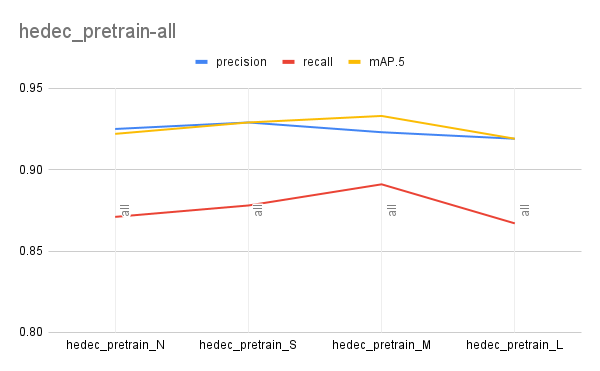
\includegraphics[width=1\textwidth]{gambar/final_weight_val/hedec_pretrain-all.png}
  \caption{Grafik \emph{Precision, Recall, mAP} untuk Bobot Hasil Pretrain COCO-YOLOv5 untuk Semua Kelas}
  \label{fig:grafval_pretrain_all}  
\end{figure}

\begin{figure} [h!]
  \centering
  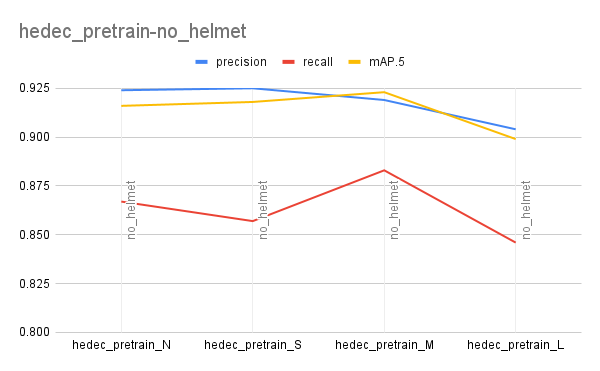
\includegraphics[width=0.49\textwidth]{gambar/final_weight_val/hedec_pretrain-no_helmet.png}
  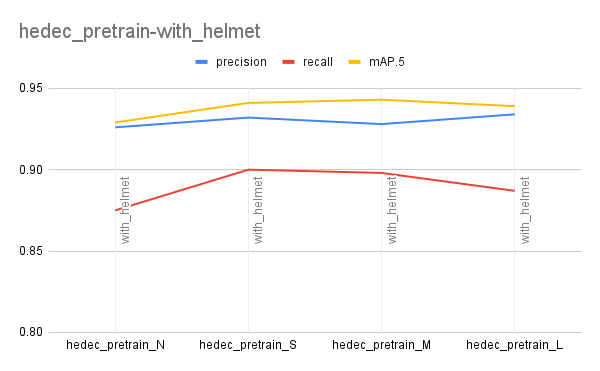
\includegraphics[width=0.49\textwidth]{gambar/final_weight_val/hedec_pretrain-with_helmet.png}
  \caption{Grafik \emph{Precision, Recall, mAP} untuk Bobot Hasil Pretrain COCO-YOLOv5 untuk Masing Masing Kelas}
  \label{fig:grafval_pretrain_eachclass}  
\end{figure}


\par Berdasarkan hasil validasi yang dipaparkan, tidak ada perbedaan signifikan dari \emph{precision, recall, mAP} 
baik pada kelas "with\_helmet" ataupun "no\_helmet" seperti yang ditunjukan pada Gambar~\ref{fig:grafval_pretrain_eachclass}.
Untuk nilai \emph{precision} berada di atas 0.9 dengan nilai tertinggi oleh varian "hedec\_pretrain\_S" . Untuk \emph{recall}
juga tidak terlalu berbeda diantara bobot dimana semuanya berada diatas angka 0.8 dengan bilai teringgi 
oleh varian "hedec\_pretrain\_M". 

\subsection{Pengujian Performa \emph{Weight} Hasil Train Murni Dataset Deteksi Helm Keselamatan Kerja}
\label{subsec:murnidataset}

\par Berikut merupakan pemaparan dari hasil validasi untuk bobot yang dilatih tanpa \emph{pretrained weights}
dari YOLOv5 . Tetapi untuk konfigurasinya dibuat serupa dengan varian \emph{Nano (N), Small (S), Medium(M),} dan \emph{Large(L)}. 
Hasil validasi dapat dilihat pada Tabel~\ref{tb:nopretrain}.


\begin{longtable}{|l|l|l|l|l|l|l|} 
  \caption{hasil Validasi \emph{Weight} dari Murni Dataset}
  \label{tb:nopretrain}\\
  \hline
  Nama Bobot                          & class        & precision & recall & mAP   & mAP .5:.95 & inference time (ms)    \\ 
  \hline
  \multirow{3}{*}{hedec\_pure\_N}     & all          & 0.918     & 0.848  & 0.909 & 0.532      & \multirow{3}{*}{1.9}   \\
                                      & no\_helmet   & 0.919     & 0.839  & 0.903 & 0.52       &                        \\
                                      & with\_helmet & 0.918     & 0.856  & 0.915 & 0.544      &                        \\ 
  \hline
  \multirow{3}{*}{hedec\_pure\_S}     & all          & 0.926     & 0.866  & 0.919 & 0.555      & \multirow{3}{*}{4.2}   \\
                                      & no\_helmet   & 0.925     & 0.86   & 0.911 & 0.55       &                        \\
                                      & with\_helmet & 0.927     & 0.872  & 0.927 & 0.559      &                        \\ 
  \hline
  \multirow{3}{*}{hedec\_pure\_M}     & all          & 0.932     & 0.866  & 0.924 & 0.564      & \multirow{3}{*}{8.9}   \\
                                      & no\_helmet   & 0.937     & 0.856  & 0.917 & 0.562      &                        \\
                                      & with\_helmet & 0.927     & 0.877  & 0.93  & 0.566      &                        \\ 
  \hline
  \multirow{3}{*}{hedec\_pure\_L}     & all          & 0.922     & 0.876  & 0.923 & 0.566      & \multirow{3}{*}{14.1}  \\
                                      & no\_helmet   & 0.919     & 0.868  & 0.914 & 0.561      &                        \\
                                      & with\_helmet & 0.925     & 0.884  & 0.932 & 0.572      &                        \\
  \hline
\end{longtable}

\begin{figure} [h!]
  \centering
  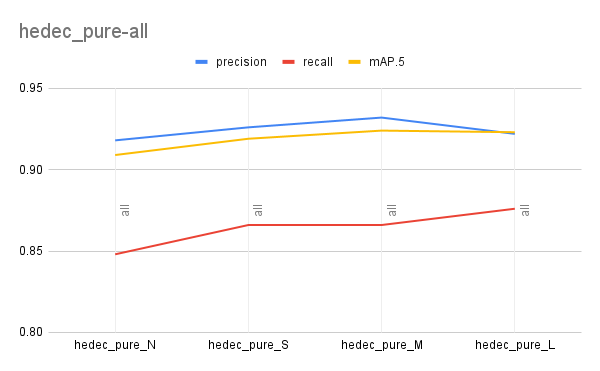
\includegraphics[width=1\textwidth]{gambar/final_weight_val/hedec_pure-all.png}
  \caption{Grafik \emph{Precision, Recall, mAP} untuk Bobot Tanpa Pretrain COCO-YOLOv5 untuk Semua Kelas}
  \label{fig:grafval_pure_all}  
\end{figure}

\begin{figure} [h!]
  \centering
  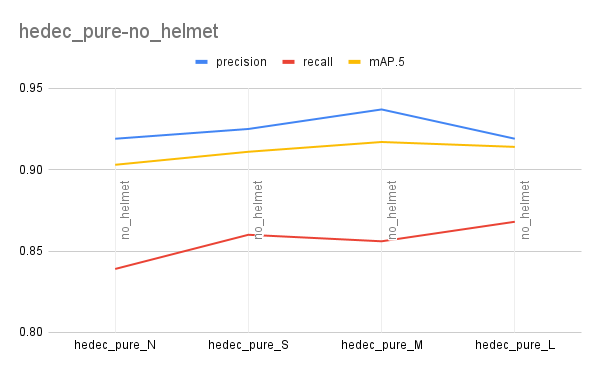
\includegraphics[width=0.4\textwidth]{gambar/final_weight_val/hedec_pure-no_helmet.png}
  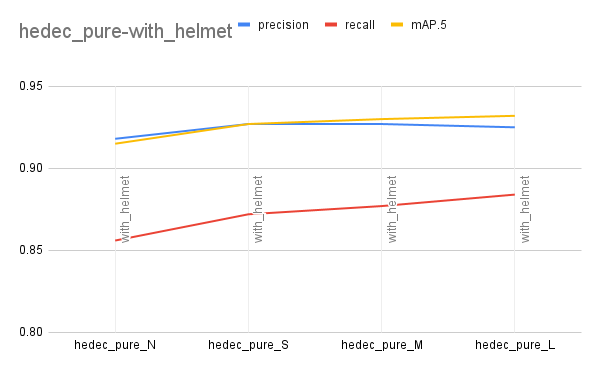
\includegraphics[width=0.4\textwidth]{gambar/final_weight_val/hedec_pure-with_helmet.png}
  \caption{Grafik \emph{Precision, Recall, mAP} untuk Bobot Tanpa Pretrain COCO-YOLOv5 untuk Kelas "no\_helmet"}
  \label{fig:grafval_pure_eachclass}  
\end{figure}

 
\newpage
\par Berdasarkan hasil validasi yang dilakukan untuk bobot - bobot yang dilatih tanpa menggunakan \emph{Pretrained Weights} dari YOLOv5
yang dapat ditarik beberapa point.Seperti yang dapat dilihat Gambar~\ref{fig:grafval_pure_all} untuk rata- rata semua kelas
dan Gambar~\ref{fig:grafval_pure_eachclass} untuk masing-masing kelas, ntuk \emph{precision} secara umum berada di atas 0.9 dan \emph{recall} di atas 0.8, begitu juga dengan
mAP.5 nya yang berada ditas 0.9. Tetapi dari segi \emph{inference time} untuk masing - masin varian, tidak ada perbedaan jauh jika dibandingkan
bobot - bobot yang di latih menggunakan \emph{Pretrained Weights} dari YOLOv5 yang dijelaskan di Sub Bab~\ref{subsec:ujiperforma_coco}.

\section{Pengujian Performa Berdasarkan Jarak}
\label{sec:ujiberdasarkanjarak}

Pada bagian ini akan memaparkan hasil deteksi pada dataset validasi yang dibagi menjadi beberapa variasi jarak dari kamera. Dataset yang digunakan meliputi 8 foto untuk masing - masing jarak.

\subsection{Pengujian Jarak dengan \emph{Pretrained Weight}}
\label{subsec:ujijarak_pretrainedweight}

\par Bagian ini memaparkan pengujian menggunakan bobot hasil \emph{training} menggunakan \emph{Pretrained Weights}
dari repo YOLOv5 yang selanjutnya disebut sebagai "hedec\_pretrain". 

\begin{enumerate}
  \item \textbf{hedec\_pretrain\_N}
  
  \par Pada pengujian menggunakan bobot "hedec\_pretrain\_N" pada perbedaan jarak seperti yang bisa dilihat di Gambar~\ref{fig:grafvaljarak_hedec_pretrain_N}, memiliki nilai
  \emph{precision} menurun mulai dari jarak 4 meter hingga 9 meter. Hal ini dikarenakan bobot ini salah memprediksi kelas "no\_helmet" sebagai "with\_helmet" pada jarak 4 meter
  dab selebihnya. Nilai \emph{recall} pada untuk kelas "no\_helmet" rendah pada jarak 1.3 meter karena ada kelas "no\_helmet" yang
  gagal diprediksi pada jarak 1.3 meter. Hasil validasi untuk bobot "hedec\_pretrain\_N" pada semua jarak dan kelas dapat dilihat pada Tabel~\ref{tb:hasiljarak_hedec_pretrain_N}

  \begin{figure} [h!]
    \centering
    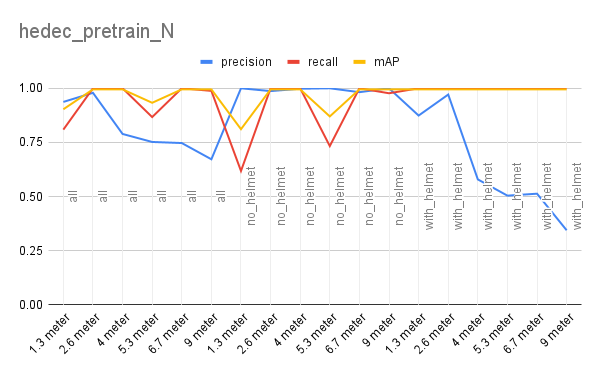
\includegraphics[width=1\textwidth]{gambar/BerdasarkanJarak/hedec_pretrain_N.png}
    \caption{Grafik \emph{Precision, Recall, mAP} untuk \textbf{"hedec\_pretrain\_N"} Pada Jarak 1.3 meter Hingga 9 meter}
    \label{fig:grafvaljarak_hedec_pretrain_N}  
  \end{figure}

 

  \begin{longtable}{|l|l|l|l|l|} 
    \caption{Hasil Validasi Perbedaan Jarak Pada \textbf{"hedec\_pretrain\_N"}}
    \label{tb:hasiljarak_hedec_pretrain_N}\\
    \hline
    Jarak     & class        & precision & recall & mAP    \\ 
    \hline
    1.3 meter & all          & 0.687     & 0.827  & 0.891  \\
    2.6 meter & all          & 0.981     & 1      & 0.995  \\
    4 meter   & all          & 0.826     & 0.988  & 0.995  \\
    5.3 meter & all          & 0.874     & 0.994  & 0.995  \\
    6.7 meter & all          & 0.858     & 0.991  & 0.995  \\
    9 meter   & all          & 0.63      & 0.933  & 0.995  \\
    1.3 meter & no\_helmet   & 1         & 0.655  & 0.995  \\
    2.6 meter & no\_helmet   & 0.989     & 1      & 0.995  \\
    4 meter   & no\_helmet   & 1         & 0.976  & 0.995  \\
    5.3 meter & no\_helmet   & 1         & 0.989  & 0.995  \\
    6.7 meter & no\_helmet   & 1         & 0.983  & 0.995  \\
    9 meter   & no\_helmet   & 1         & 0.866  & 0.995  \\
    1.3 meter & with\_helmet & 0.374     & 1      & 0.787  \\
    2.6 meter & with\_helmet & 0.973     & 1      & 0.995  \\
    4 meter   & with\_helmet & 0.651     & 1      & 0.995  \\
    5.3 meter & with\_helmet & 0.747     & 1      & 0.995  \\
    6.7 meter & with\_helmet & 0.716     & 1      & 0.995  \\
    9 meter   & with\_helmet & 0.26      & 1      & 0.995  \\
    \hline
  \end{longtable}

  \begin{figure} [h!]
    \centering
    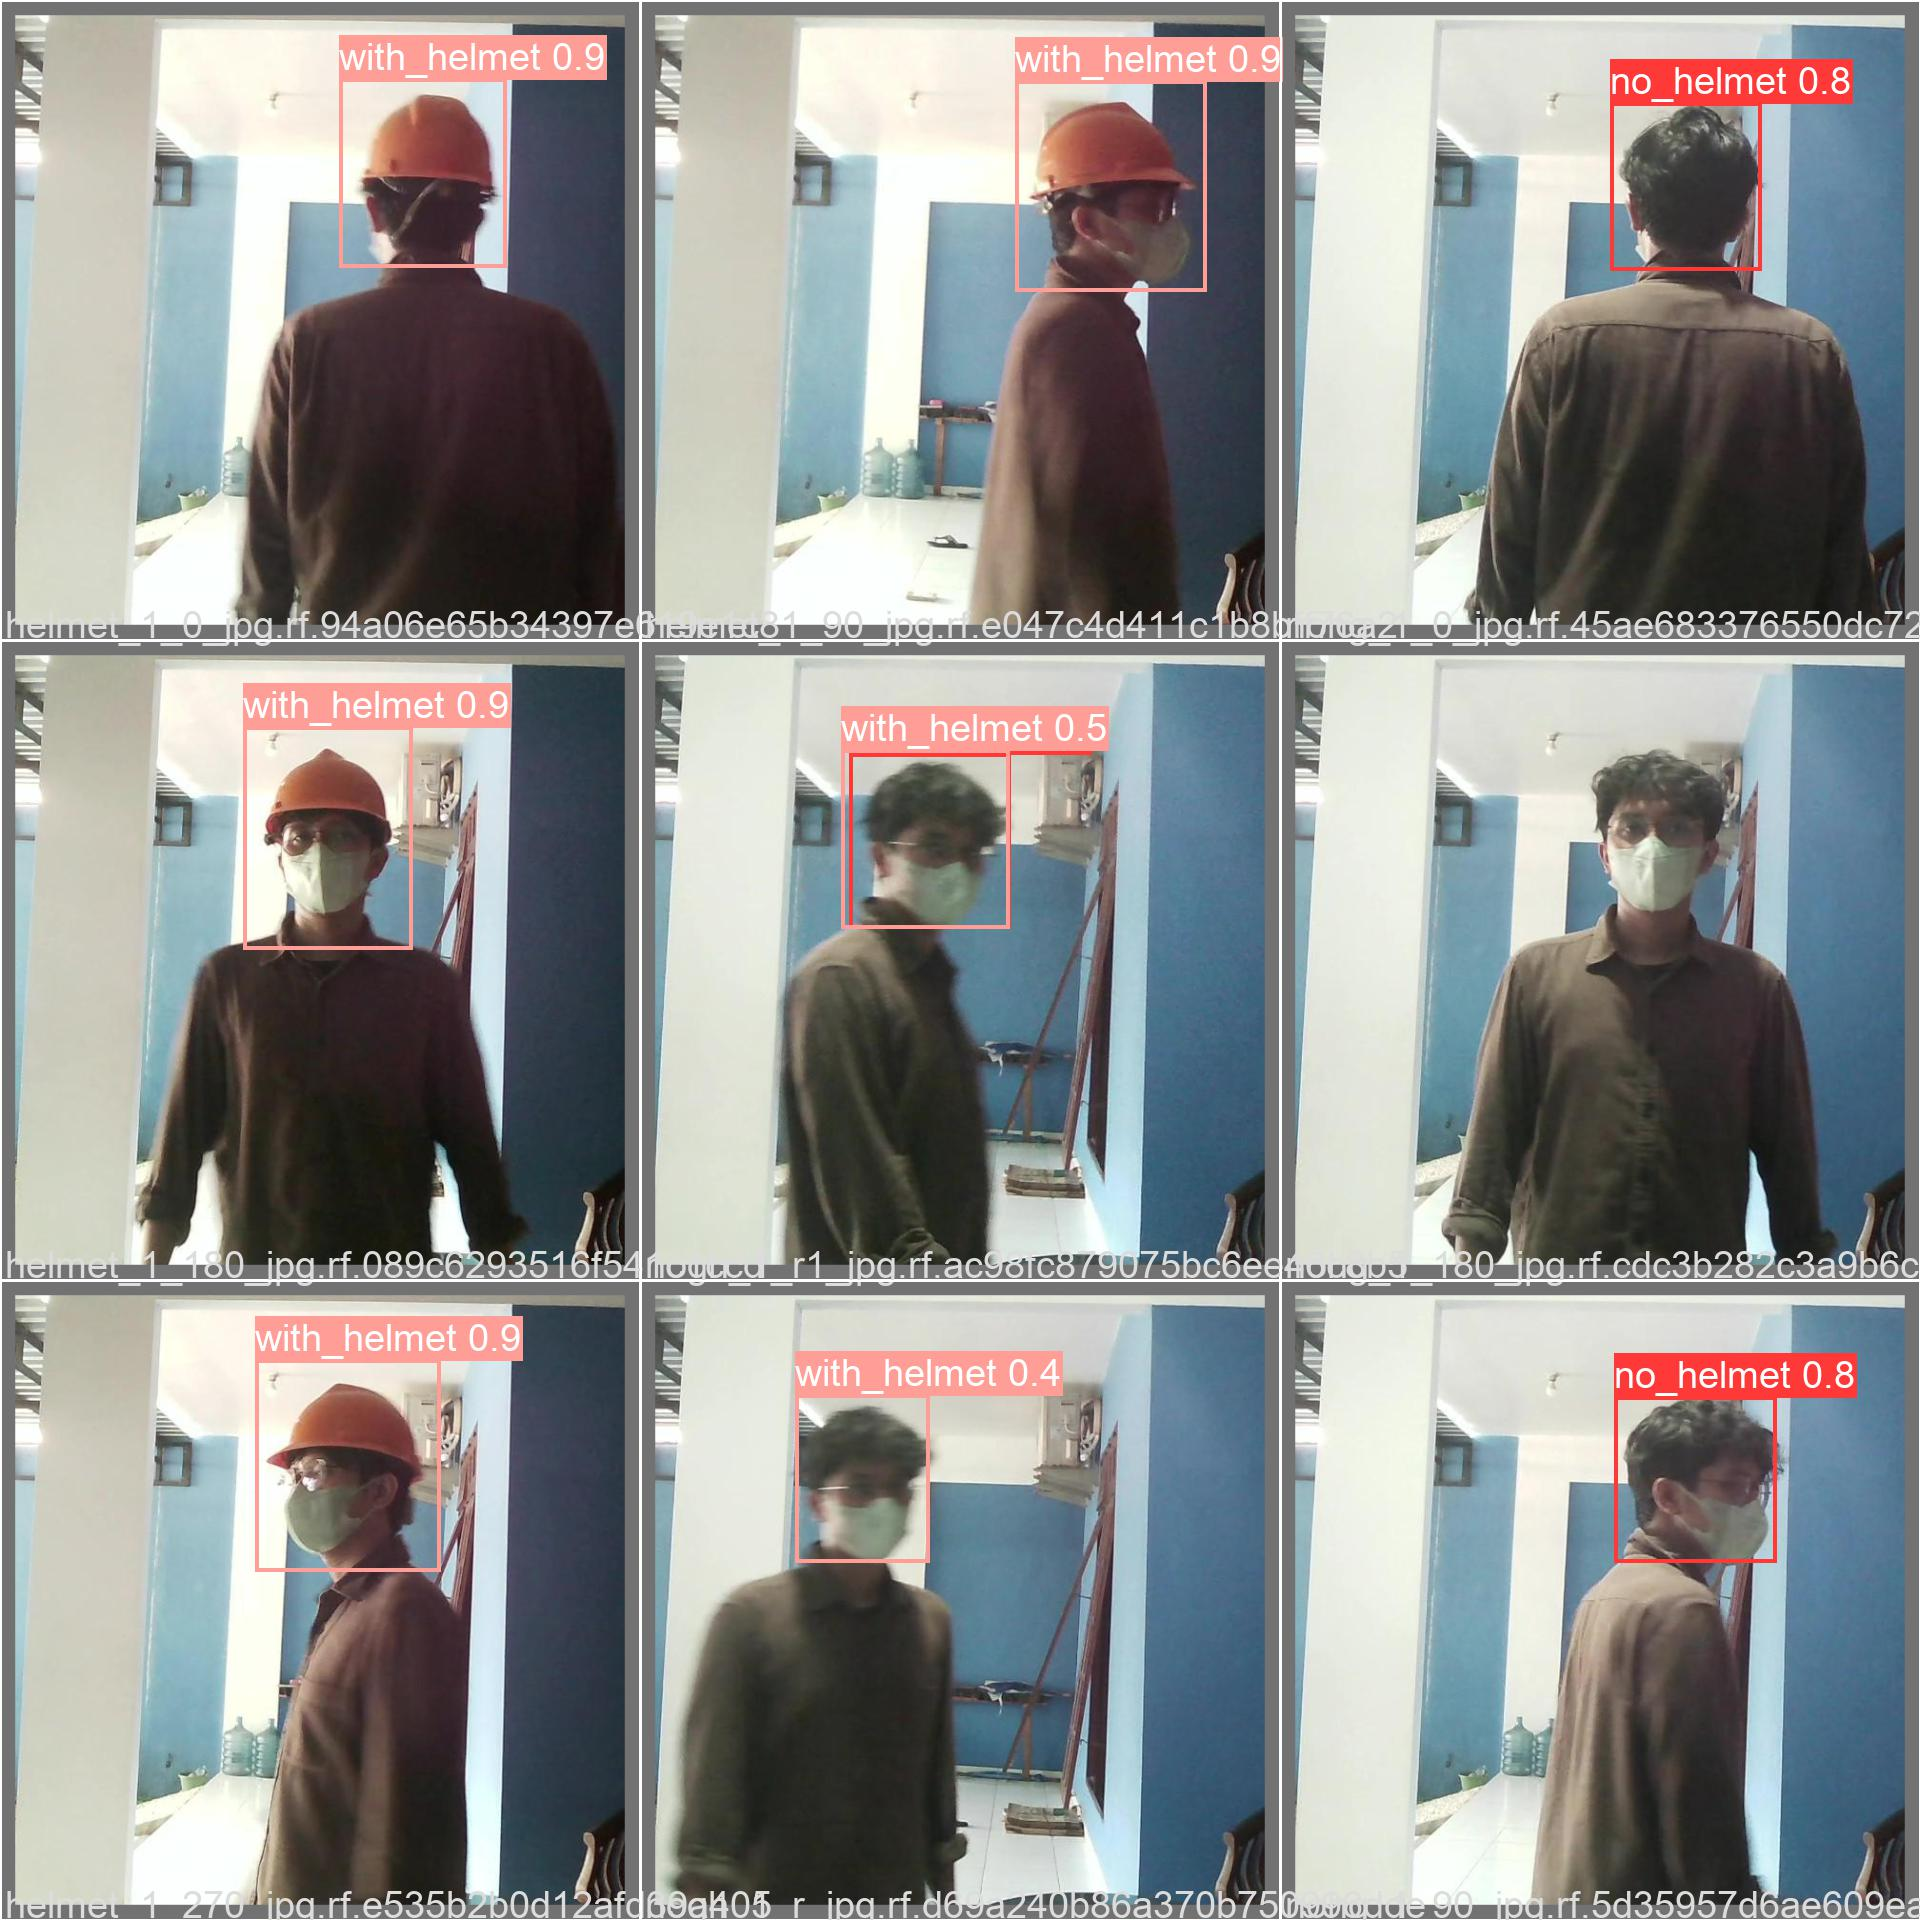
\includegraphics[width=0.3\textwidth]{gambar/BerdasarkanJarak_v2/val_hedec_pretrain_N/Jarak1_3/val_batch0_pred.jpg}
    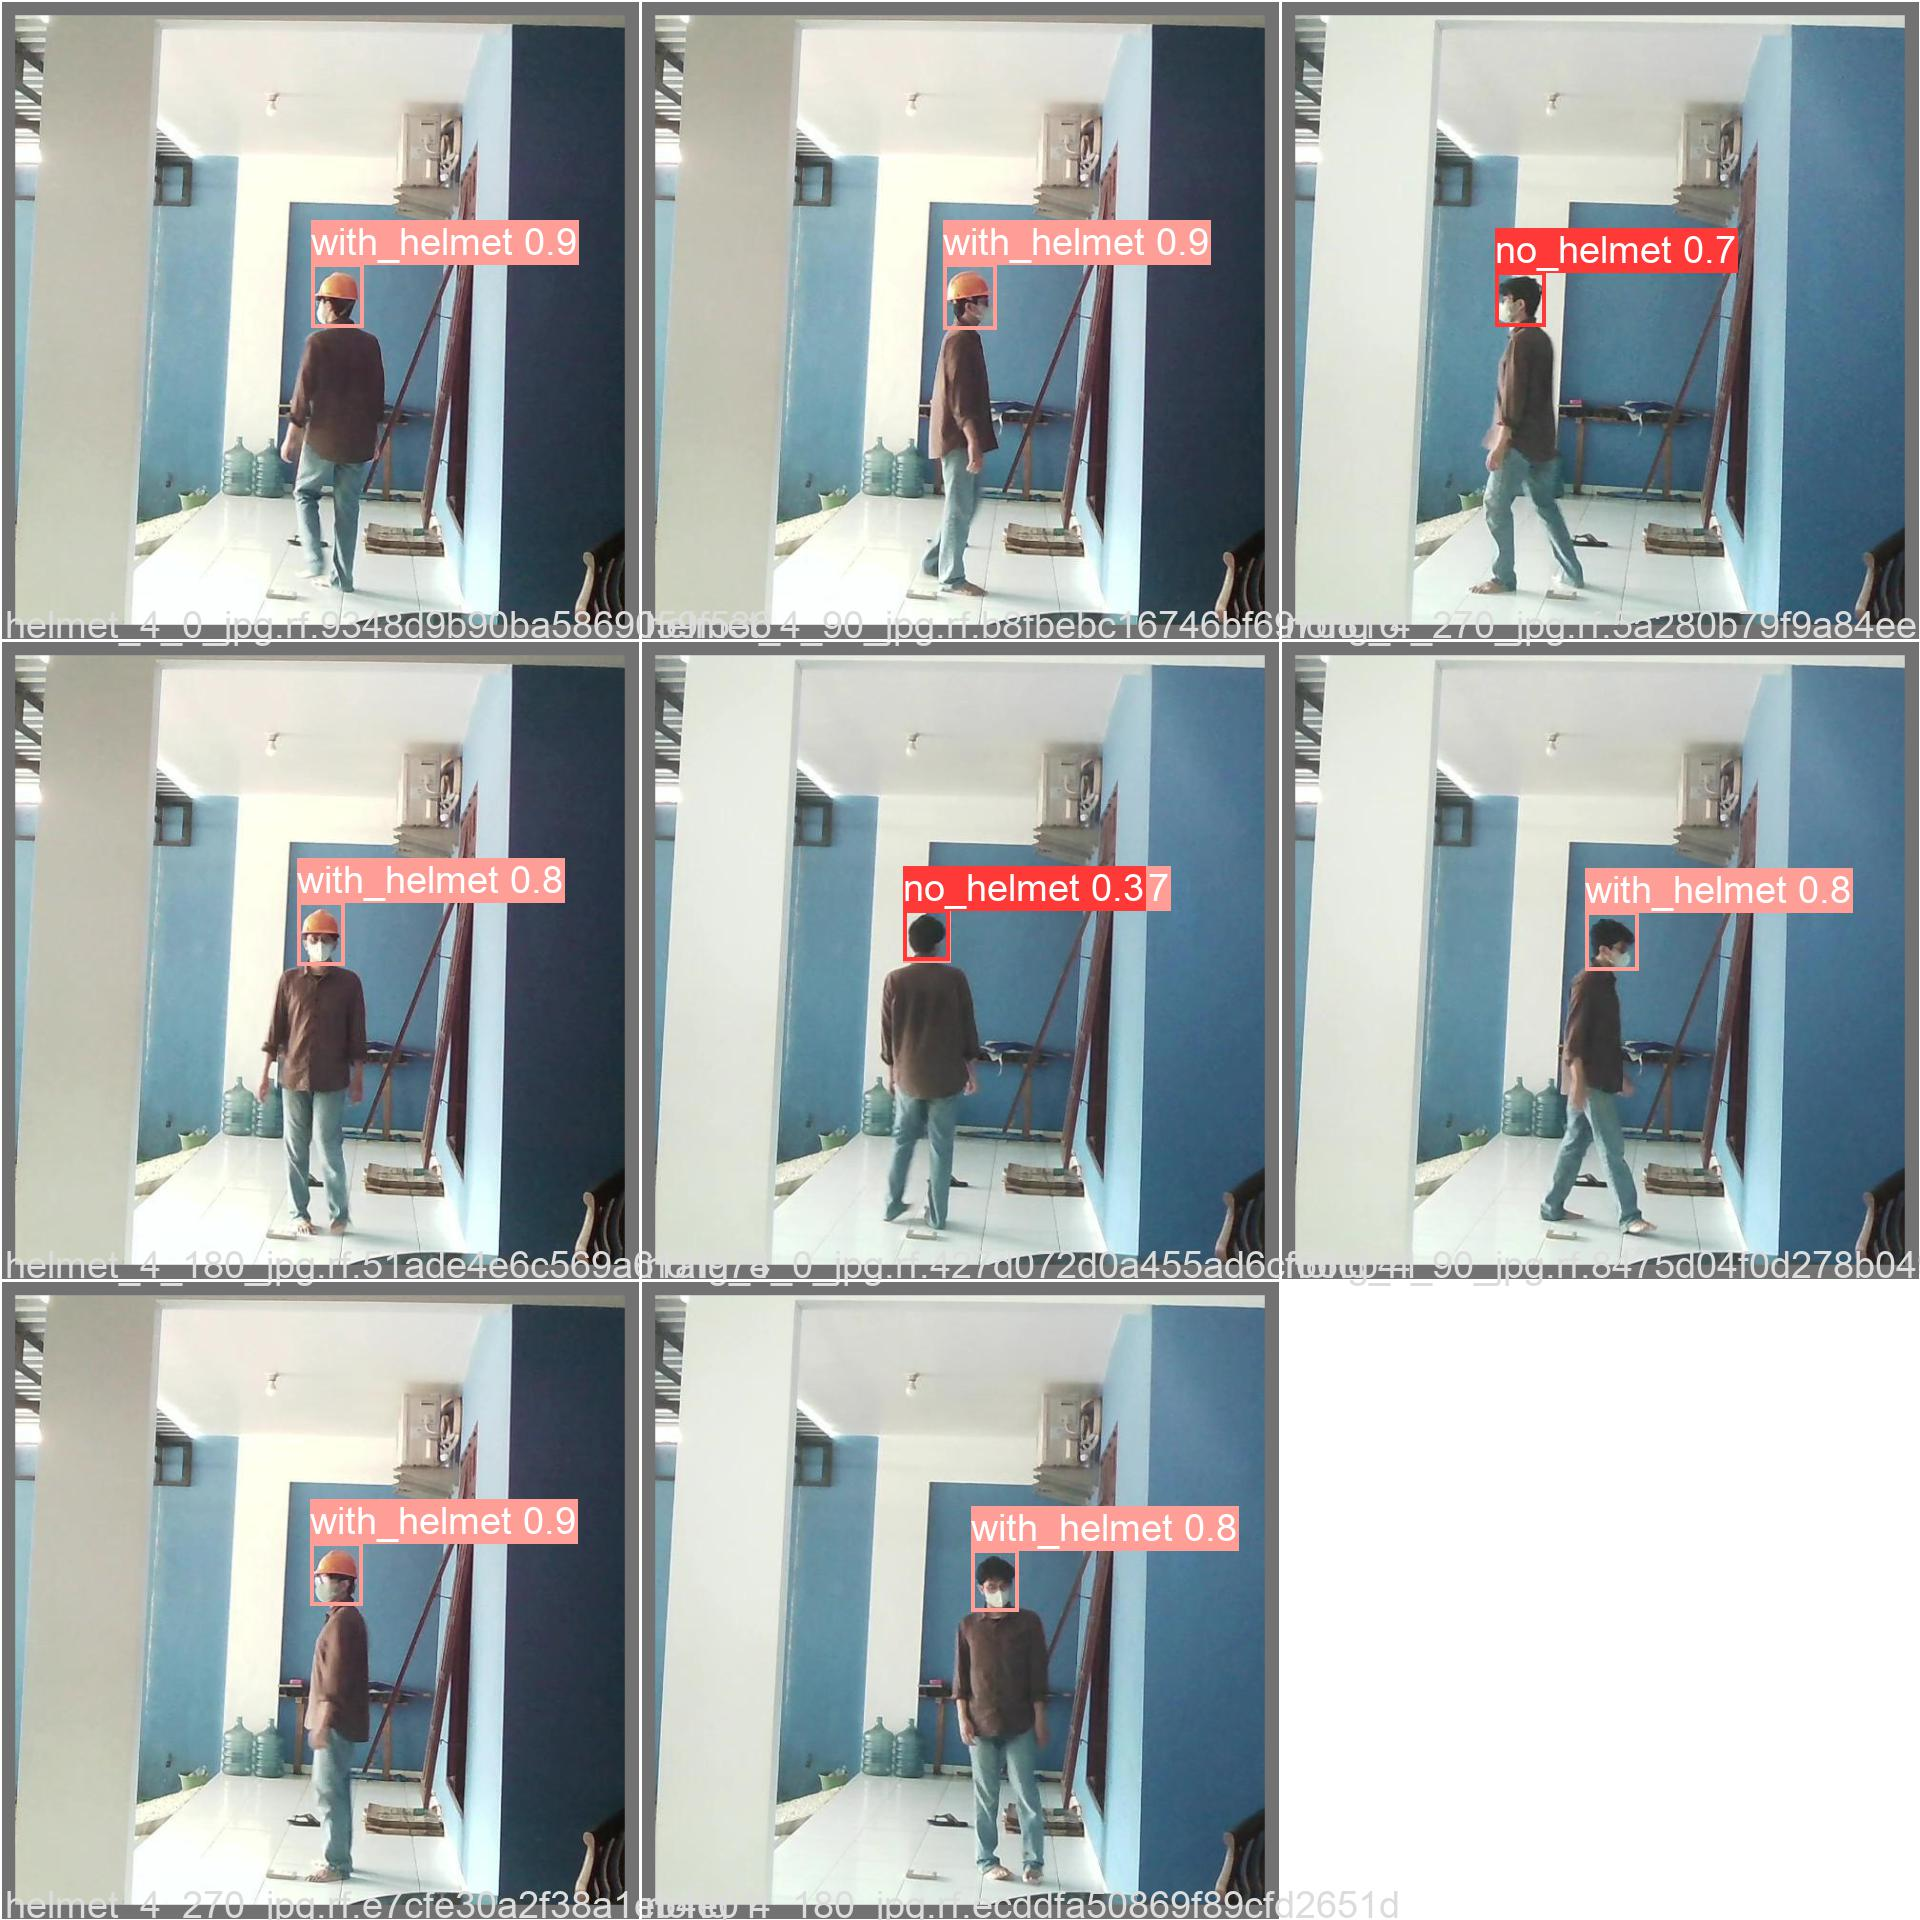
\includegraphics[width=0.3\textwidth]{gambar/BerdasarkanJarak_v2/val_hedec_pretrain_N/Jarak5_3/val_batch0_pred.jpg}
    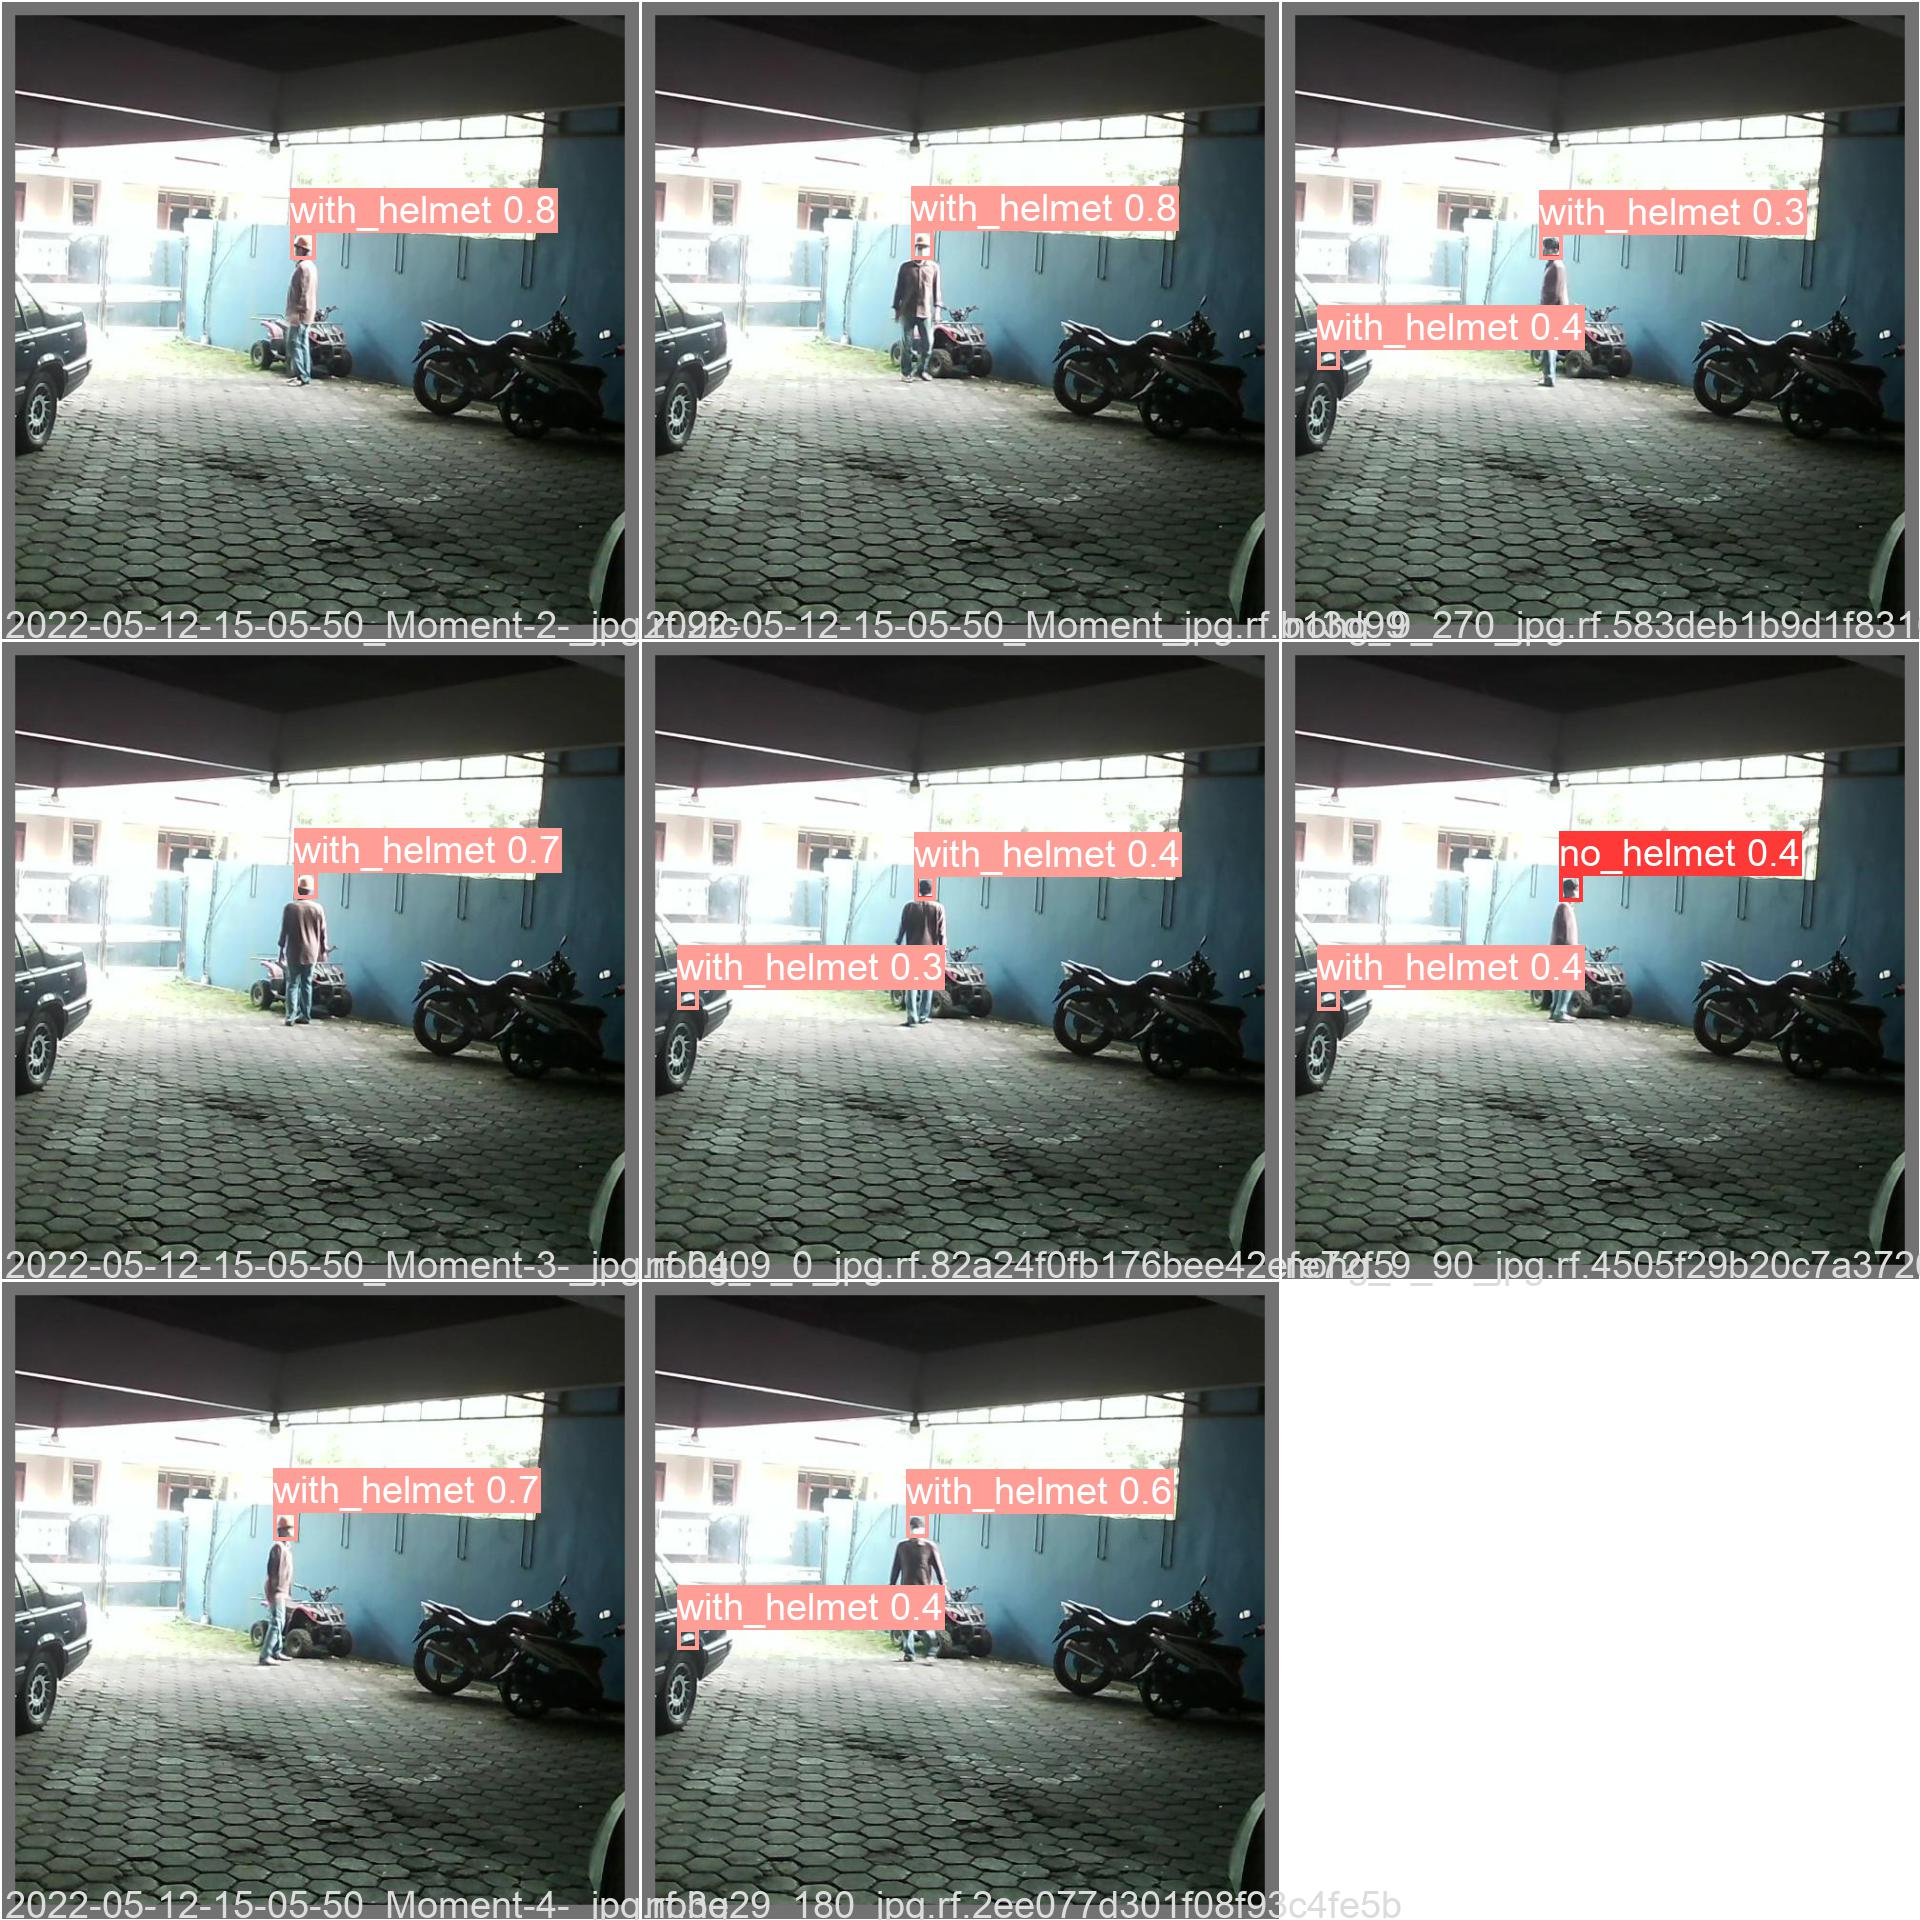
\includegraphics[width=0.3\textwidth]{gambar/BerdasarkanJarak_v2/val_hedec_pretrain_N/Jarak9/val_batch0_pred.jpg}
    \caption{Hasil Prediksi Untuk Bobot "hedec\_pretrain\_N" Pada Perbedaan Jarak}
    \label{fig:valjarak_sample_hedec_pretrain_N}  
  \end{figure}


  \item \textbf{hedec\_pretrain\_S}
  
  \par Pada pengujian jarak menggunakan bobot "hedec\_pretrain\_S", didapati bahwa bobot ini memiliki nilai metrik
  yang lebih baik daripada "hedec\_pretrain\_M". Nilai \emph{precision} rata-rata semua kelas paling rendah berada pada jarak 1.3 meter karena
  nilai \emph{precision} untuk kelas "with\_helmet" berada pada angka 0.686 dan \emph{recall} untuk kelas "no\_helmet" 0.8 karena ada beberapa 
  kelas "no\_helmet" yang salah terdeteksi sebagai "with\_helmet".

   
  \begin{longtable}{|l|l|l|l|l|} 
    \caption{Hasil Validasi Perbedaan Jarak Pada \textbf{"hedec\_pretrain\_S"}}
    \label{tb:hasiljarak_hedec_pretrain_S}\\
    \hline
    Jarak     & class        & precision & recall & mAP    \\ 
    \hline
    1.3 meter & all          & 0.843     & 0.907  & 0.995  \\
    2.6 meter & all          & 0.985     & 1      & 0.995  \\
    4 meter   & all          & 0.973     & 1      & 0.995  \\
    5.3 meter & all          & 0.986     & 1      & 0.995  \\
    6.7 meter & all          & 0.981     & 1      & 0.995  \\
    9 meter   & all          & 0.957     & 1      & 0.995  \\
    1.3 meter & no\_helmet   & 1         & 0.815  & 0.995  \\
    2.6 meter & no\_helmet   & 0.989     & 1      & 0.995  \\
    4 meter   & no\_helmet   & 0.988     & 1      & 0.995  \\
    5.3 meter & no\_helmet   & 0.988     & 1      & 0.995  \\
    6.7 meter & no\_helmet   & 0.988     & 1      & 0.995  \\
    9 meter   & no\_helmet   & 0.998     & 1      & 0.995  \\
    1.3 meter & with\_helmet & 0.686     & 1      & 0.995  \\
    2.6 meter & with\_helmet & 0.981     & 1      & 0.995  \\
    4 meter   & with\_helmet & 0.958     & 1      & 0.995  \\
    5.3 meter & with\_helmet & 0.984     & 1      & 0.995  \\
    6.7 meter & with\_helmet & 0.974     & 1      & 0.995  \\
    9 meter   & with\_helmet & 0.916     & 1      & 0.995  \\
    \hline
  \end{longtable}

  \begin{figure}[h!]
    \centering
    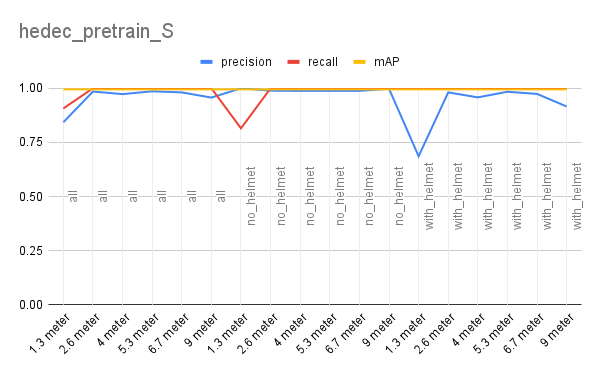
\includegraphics[width=1\textwidth]{gambar/BerdasarkanJarak/hedec_pretrain_S.png}
    \caption{Grafik \emph{Precision, Recall, mAP} untuk \textbf{"hedec\_pretrain\_S"} Pada Jarak 1.3 meter Hingga 9 meter}
    \label{fig:grafvaljarak_hedec_pretrain_S}  
  \end{figure}

  \begin{figure} [h!]
    \centering
    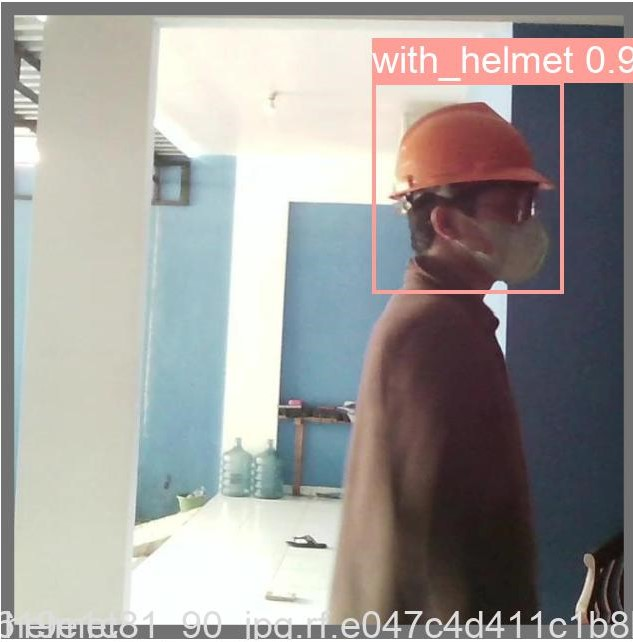
\includegraphics[width=0.3\textwidth]{gambar/BerdasarkanJarak_v2/val_hedec_pretrain_S/Jarak1_3/val_batch0_pred.jpg}
    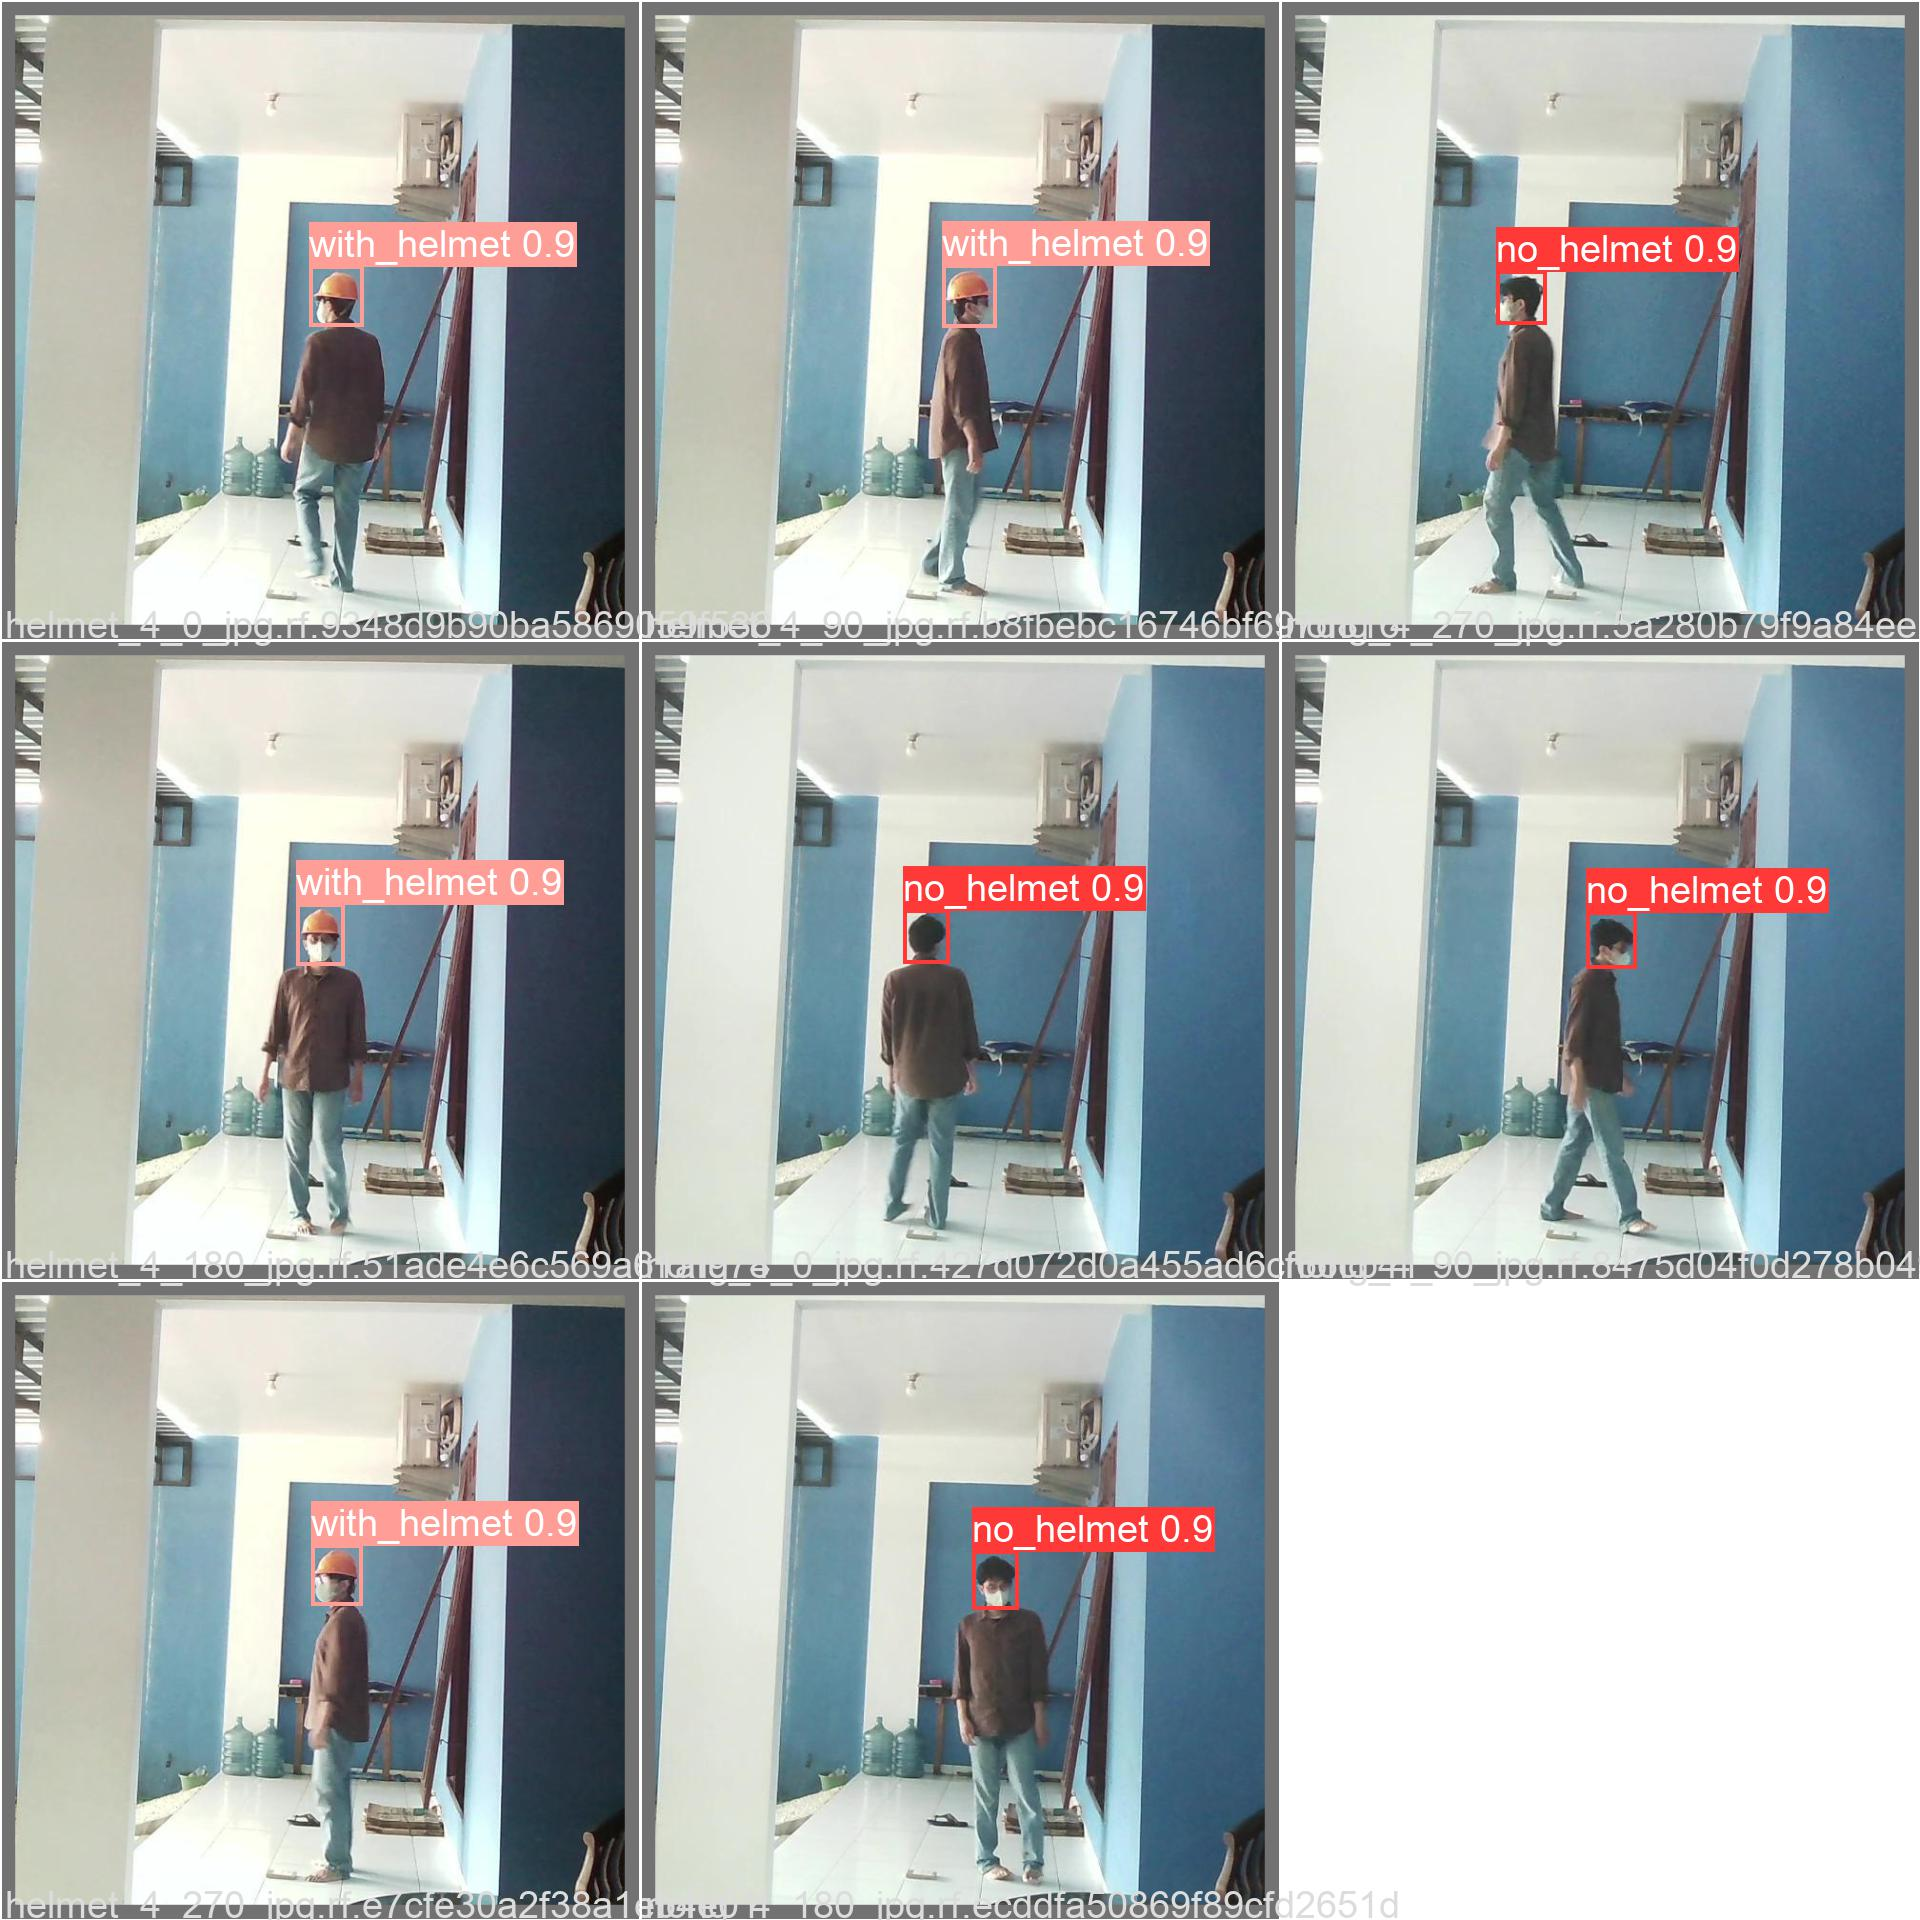
\includegraphics[width=0.3\textwidth]{gambar/BerdasarkanJarak_v2/val_hedec_pretrain_S/Jarak5_3/val_batch0_pred.jpg}
    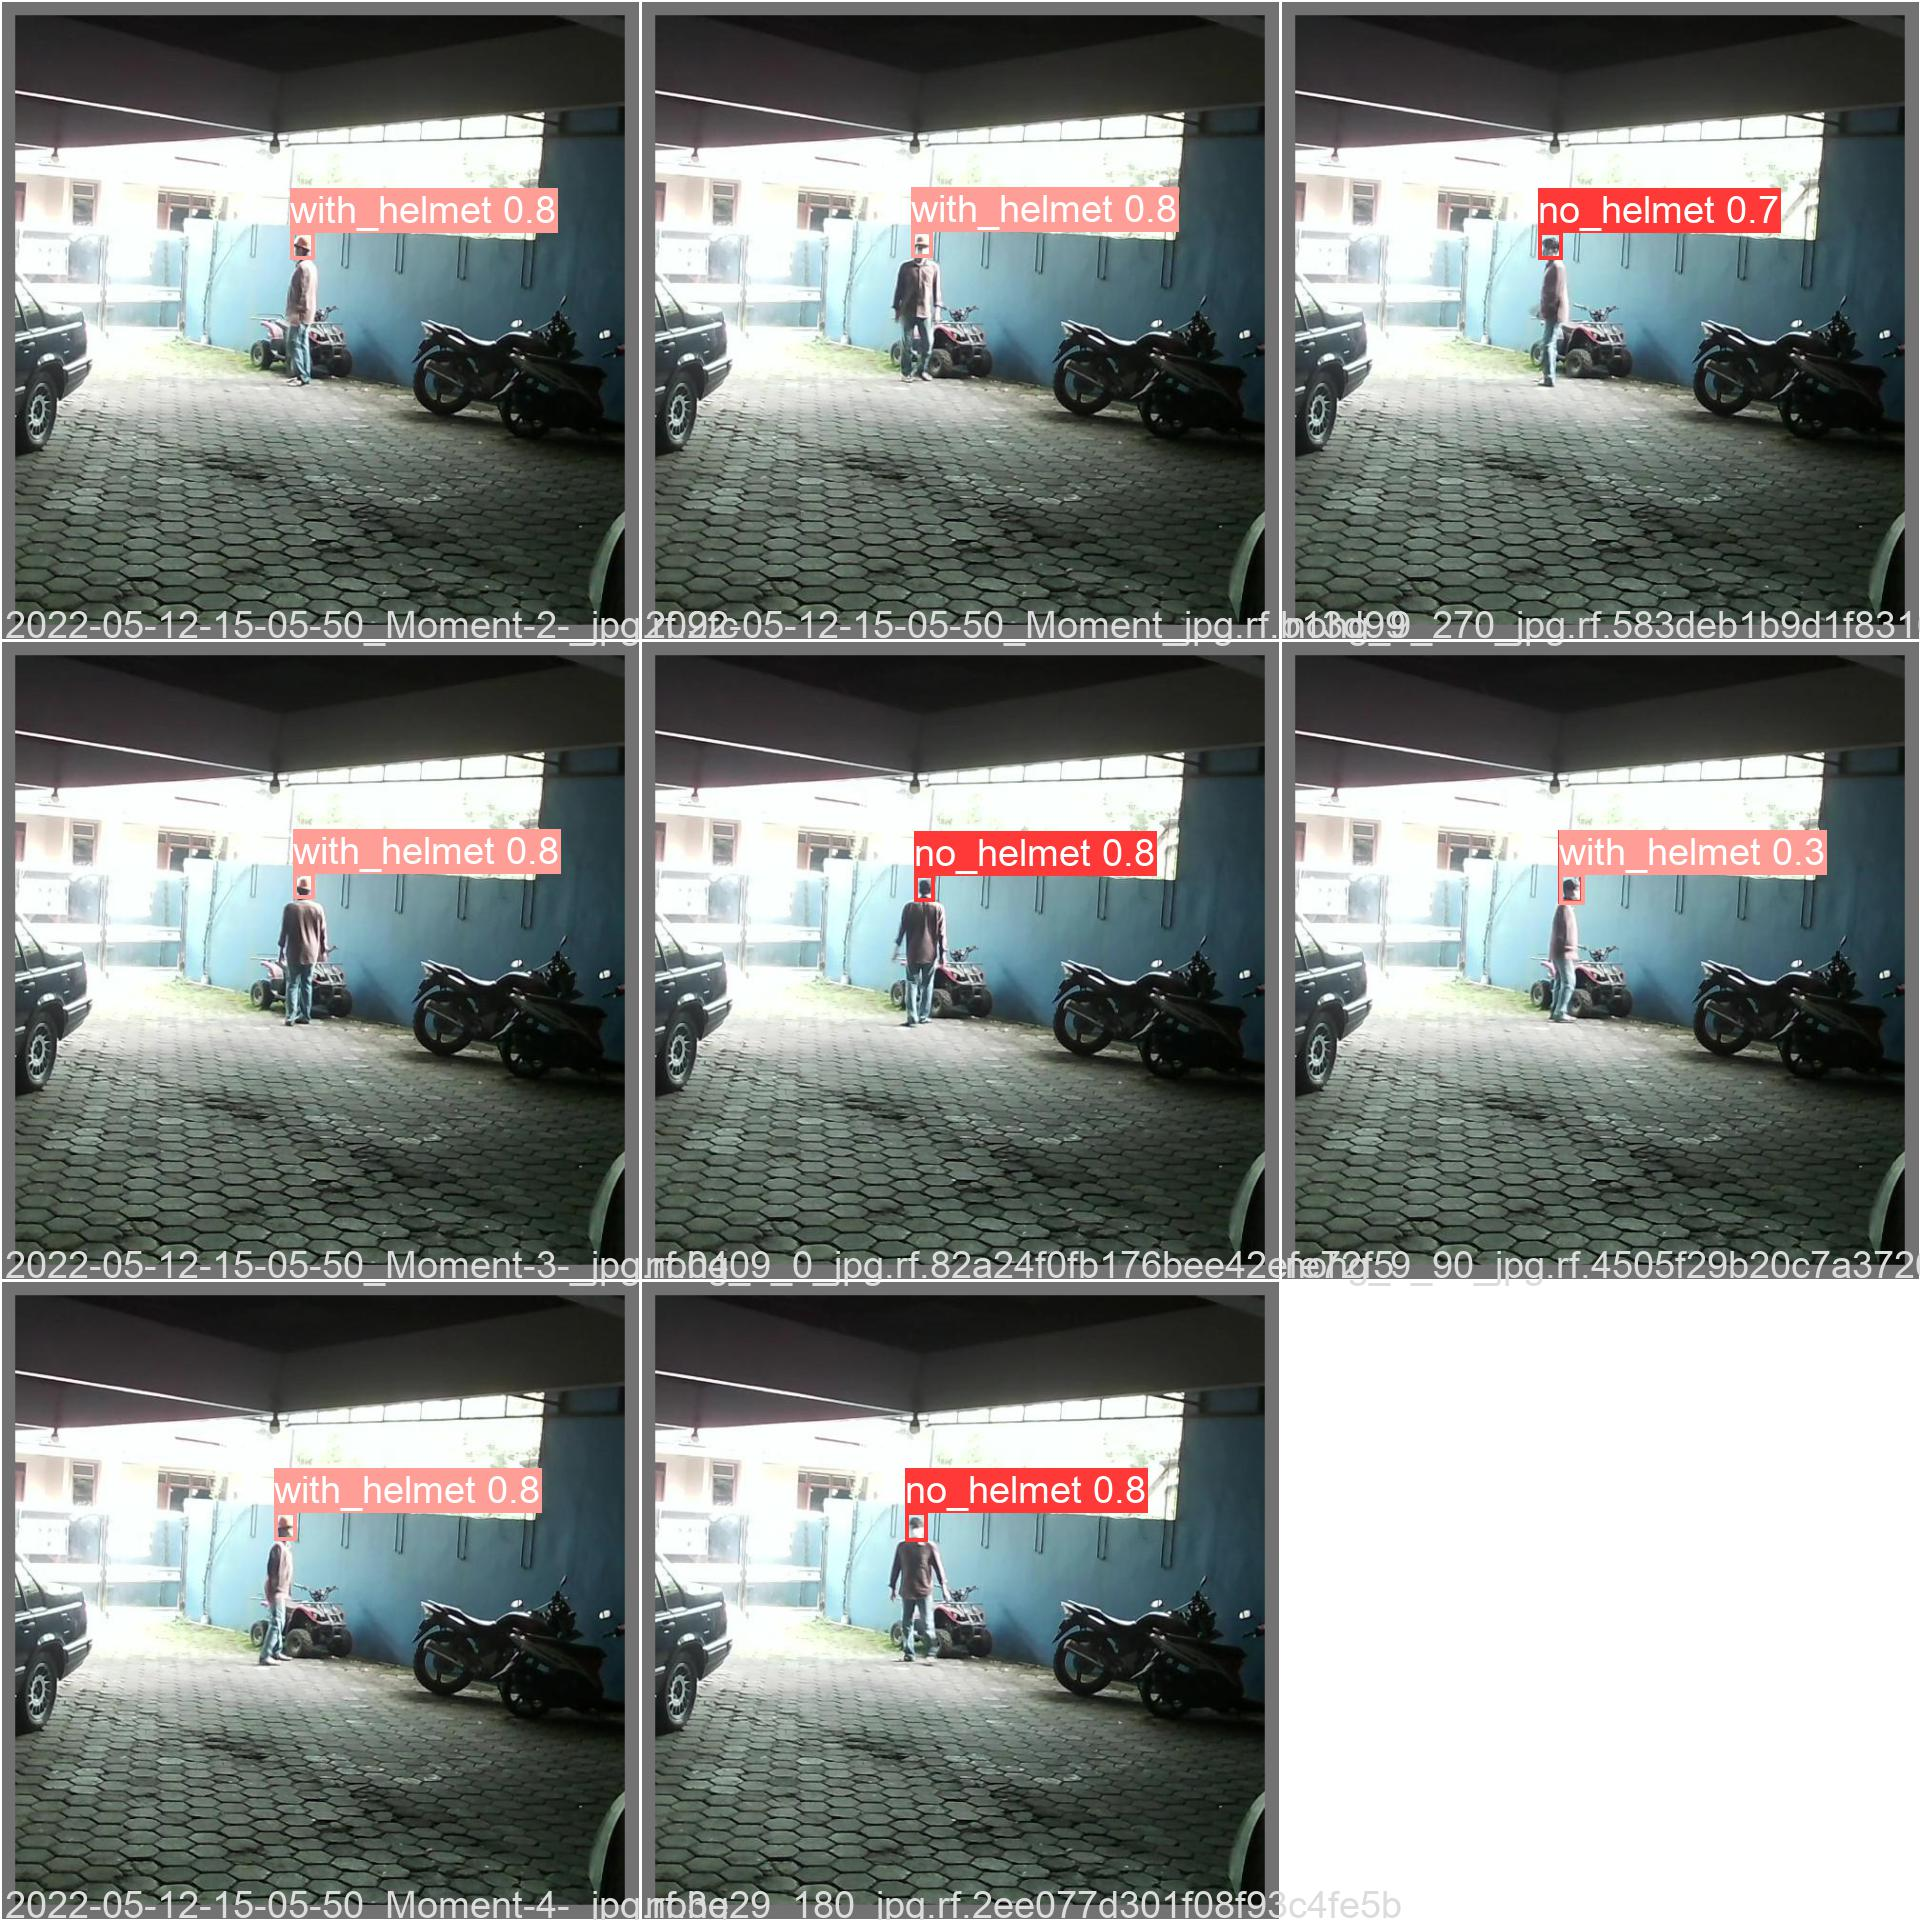
\includegraphics[width=0.3\textwidth]{gambar/BerdasarkanJarak_v2/val_hedec_pretrain_S/Jarak9/val_batch0_pred.jpg}
    \caption{Hasil Prediksi Untuk Bobot "hedec\_pretrain\_S" Pada Perbedaan Jarak}
    \label{fig:valjarak_sample_hedec_pretrain_S}  
  \end{figure}

  \FloatBarrier
  
   
  \item \textbf{hedec\_pretrain\_M}
  
  \par Pada pengujian menggunakan bobot "hedec\_pretrain\_M" pada perbedaan jarak seperti yang bisa dilihat di Gambar~\ref{fig:grafvaljarak_hedec_pretrain_M}, jarak 1.3 meter dan 9 meter
  secara umum memiliki nilai yang sangat buruk. Pada jarak 1.3 meter, nilai \emph{precision} untuk kelas "with\_helmet"
  mencapai nilai 0.374 sedangkan pada jarak 9 meter mendapatkan nilai 0.26. Untuk kelas "no\_helmet" untuk semua jarak memiliki
  nilai yang bagus diatas 0.9 untuk presisinya. Terlihat untuk \emph{weight} ini mengalami kesulitan untuk mendeteksi
  kelas "with\_helmet" pada jarak 1.3 meter dan pada jarak 9 meter.


  \begin{longtable}{|l|l|l|l|l|} 
    \caption{Hasil Validasi Perbedaan Jarak Pada \textbf{"hedec\_pretrain\_M"}}
    \label{tb:hasiljarak_hedec_pretrain_M}\\
    \hline
    Jarak     & class        & precision & recall & mAP    \\ 
    \hline
    1.3 meter & all          & 0.687     & 0.827  & 0.891  \\
    2.6 meter & all          & 0.981     & 1      & 0.995  \\
    4 meter   & all          & 0.826     & 0.988  & 0.995  \\
    5.3 meter & all          & 0.874     & 0.994  & 0.995  \\
    6.7 meter & all          & 0.858     & 0.991  & 0.995  \\
    9 meter   & all          & 0.63      & 0.933  & 0.995  \\
    1.3 meter & no\_helmet   & 1         & 0.655  & 0.995  \\
    2.6 meter & no\_helmet   & 0.989     & 1      & 0.995  \\
    4 meter   & no\_helmet   & 1         & 0.976  & 0.995  \\
    5.3 meter & no\_helmet   & 1         & 0.989  & 0.995  \\
    6.7 meter & no\_helmet   & 1         & 0.983  & 0.995  \\
    9 meter   & no\_helmet   & 1         & 0.866  & 0.995  \\
    1.3 meter & with\_helmet & 0.374     & 1      & 0.787  \\
    2.6 meter & with\_helmet & 0.973     & 1      & 0.995  \\
    4 meter   & with\_helmet & 0.651     & 1      & 0.995  \\
    5.3 meter & with\_helmet & 0.747     & 1      & 0.995  \\
    6.7 meter & with\_helmet & 0.716     & 1      & 0.995  \\
    9 meter   & with\_helmet & 0.26      & 1      & 0.995  \\
    \hline
  \end{longtable}

  \begin{figure} [h!]
    \centering
    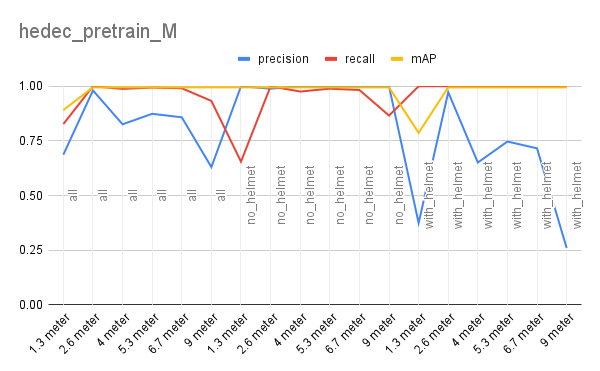
\includegraphics[width=1\textwidth]{gambar/BerdasarkanJarak/hedec_pretrain_M.png}
    \caption{Grafik \emph{Precision, Recall, mAP} untuk \textbf{"hedec\_pretrain\_M"} Pada Jarak 1.3 meter Hingga 9 meter}
    \label{fig:grafvaljarak_hedec_pretrain_M}  
  \end{figure}

  \FloatBarrier

  \begin{figure} [h!]
    \centering
    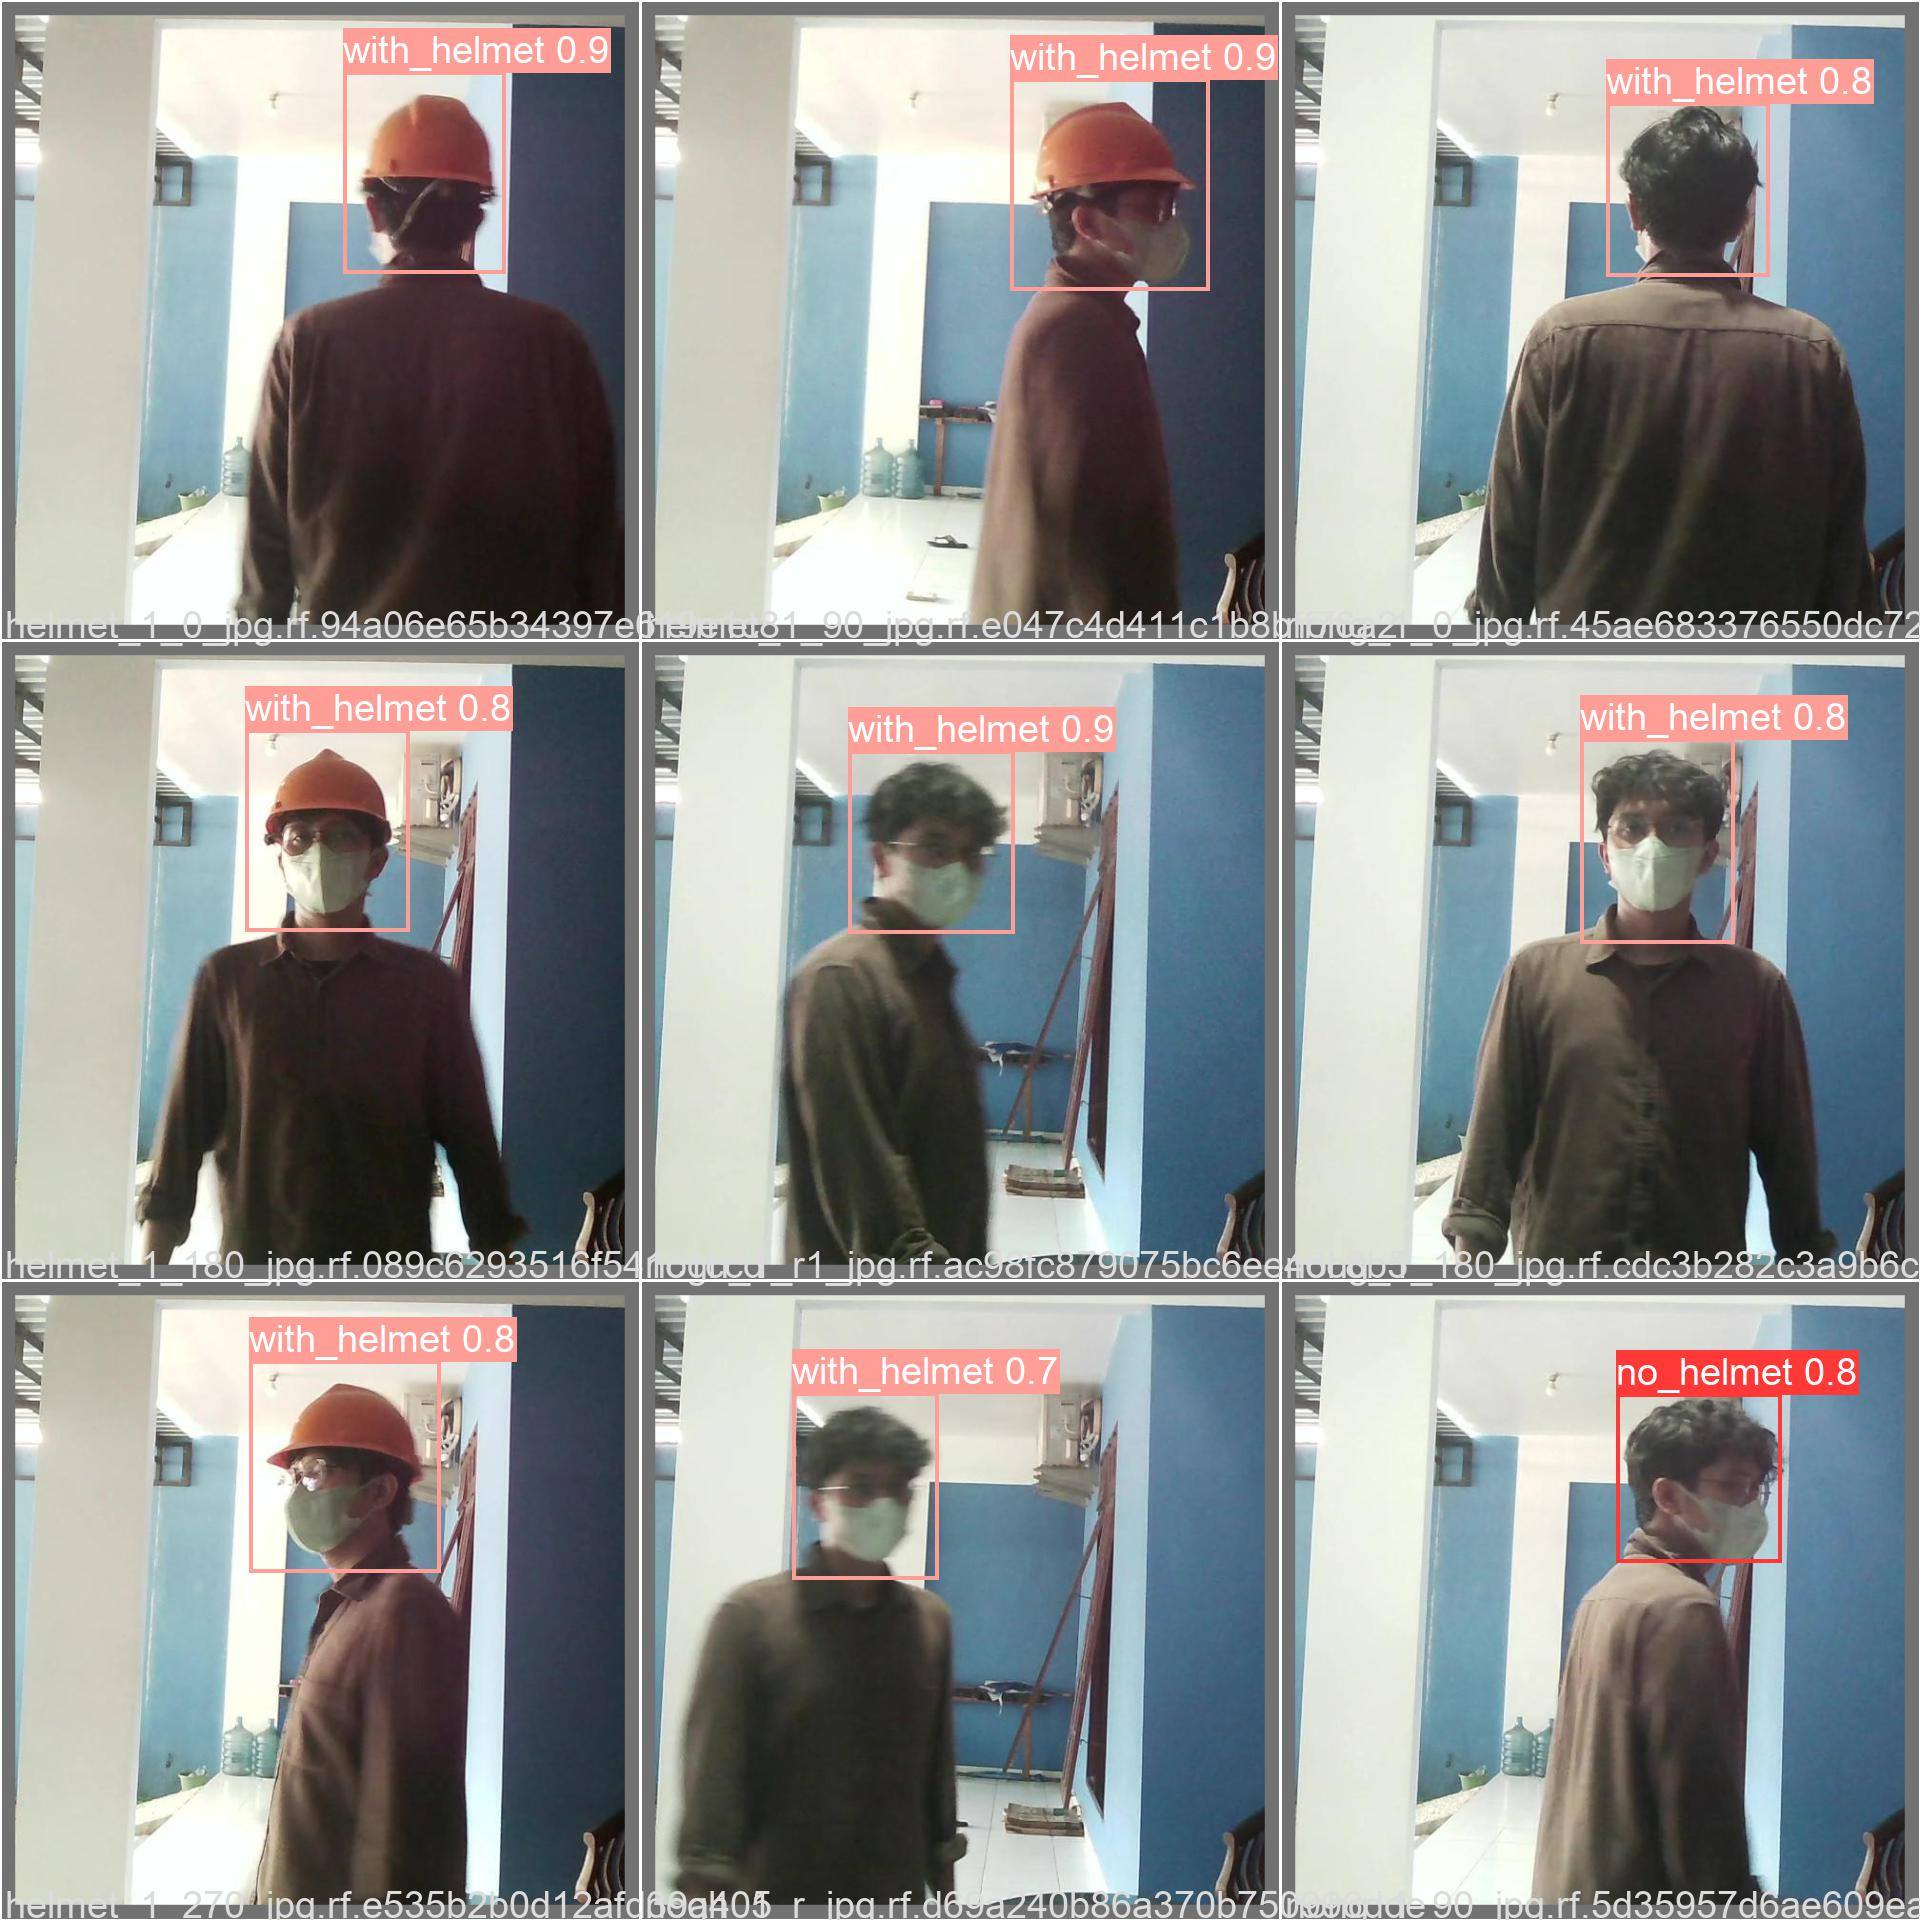
\includegraphics[width=0.3\textwidth]{gambar/BerdasarkanJarak_v2/val_hedec_pretrain_M/Jarak1_3/val_batch0_pred.jpg}
    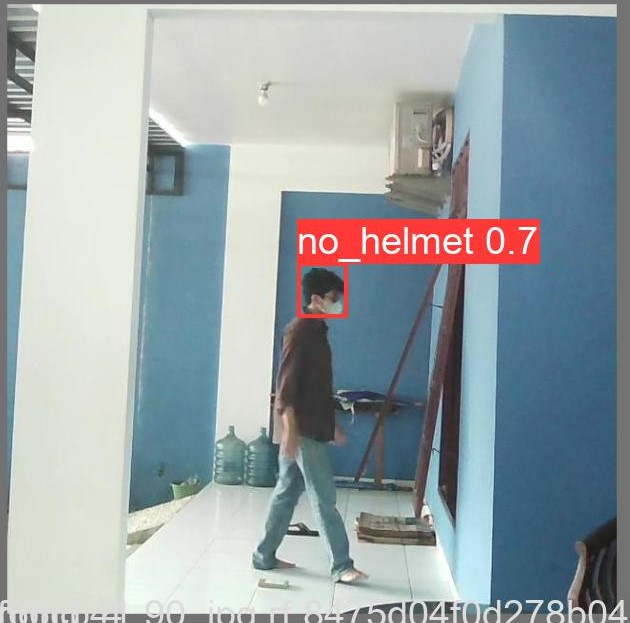
\includegraphics[width=0.3\textwidth]{gambar/BerdasarkanJarak_v2/val_hedec_pretrain_M/Jarak5_3/val_batch0_pred.jpg}
    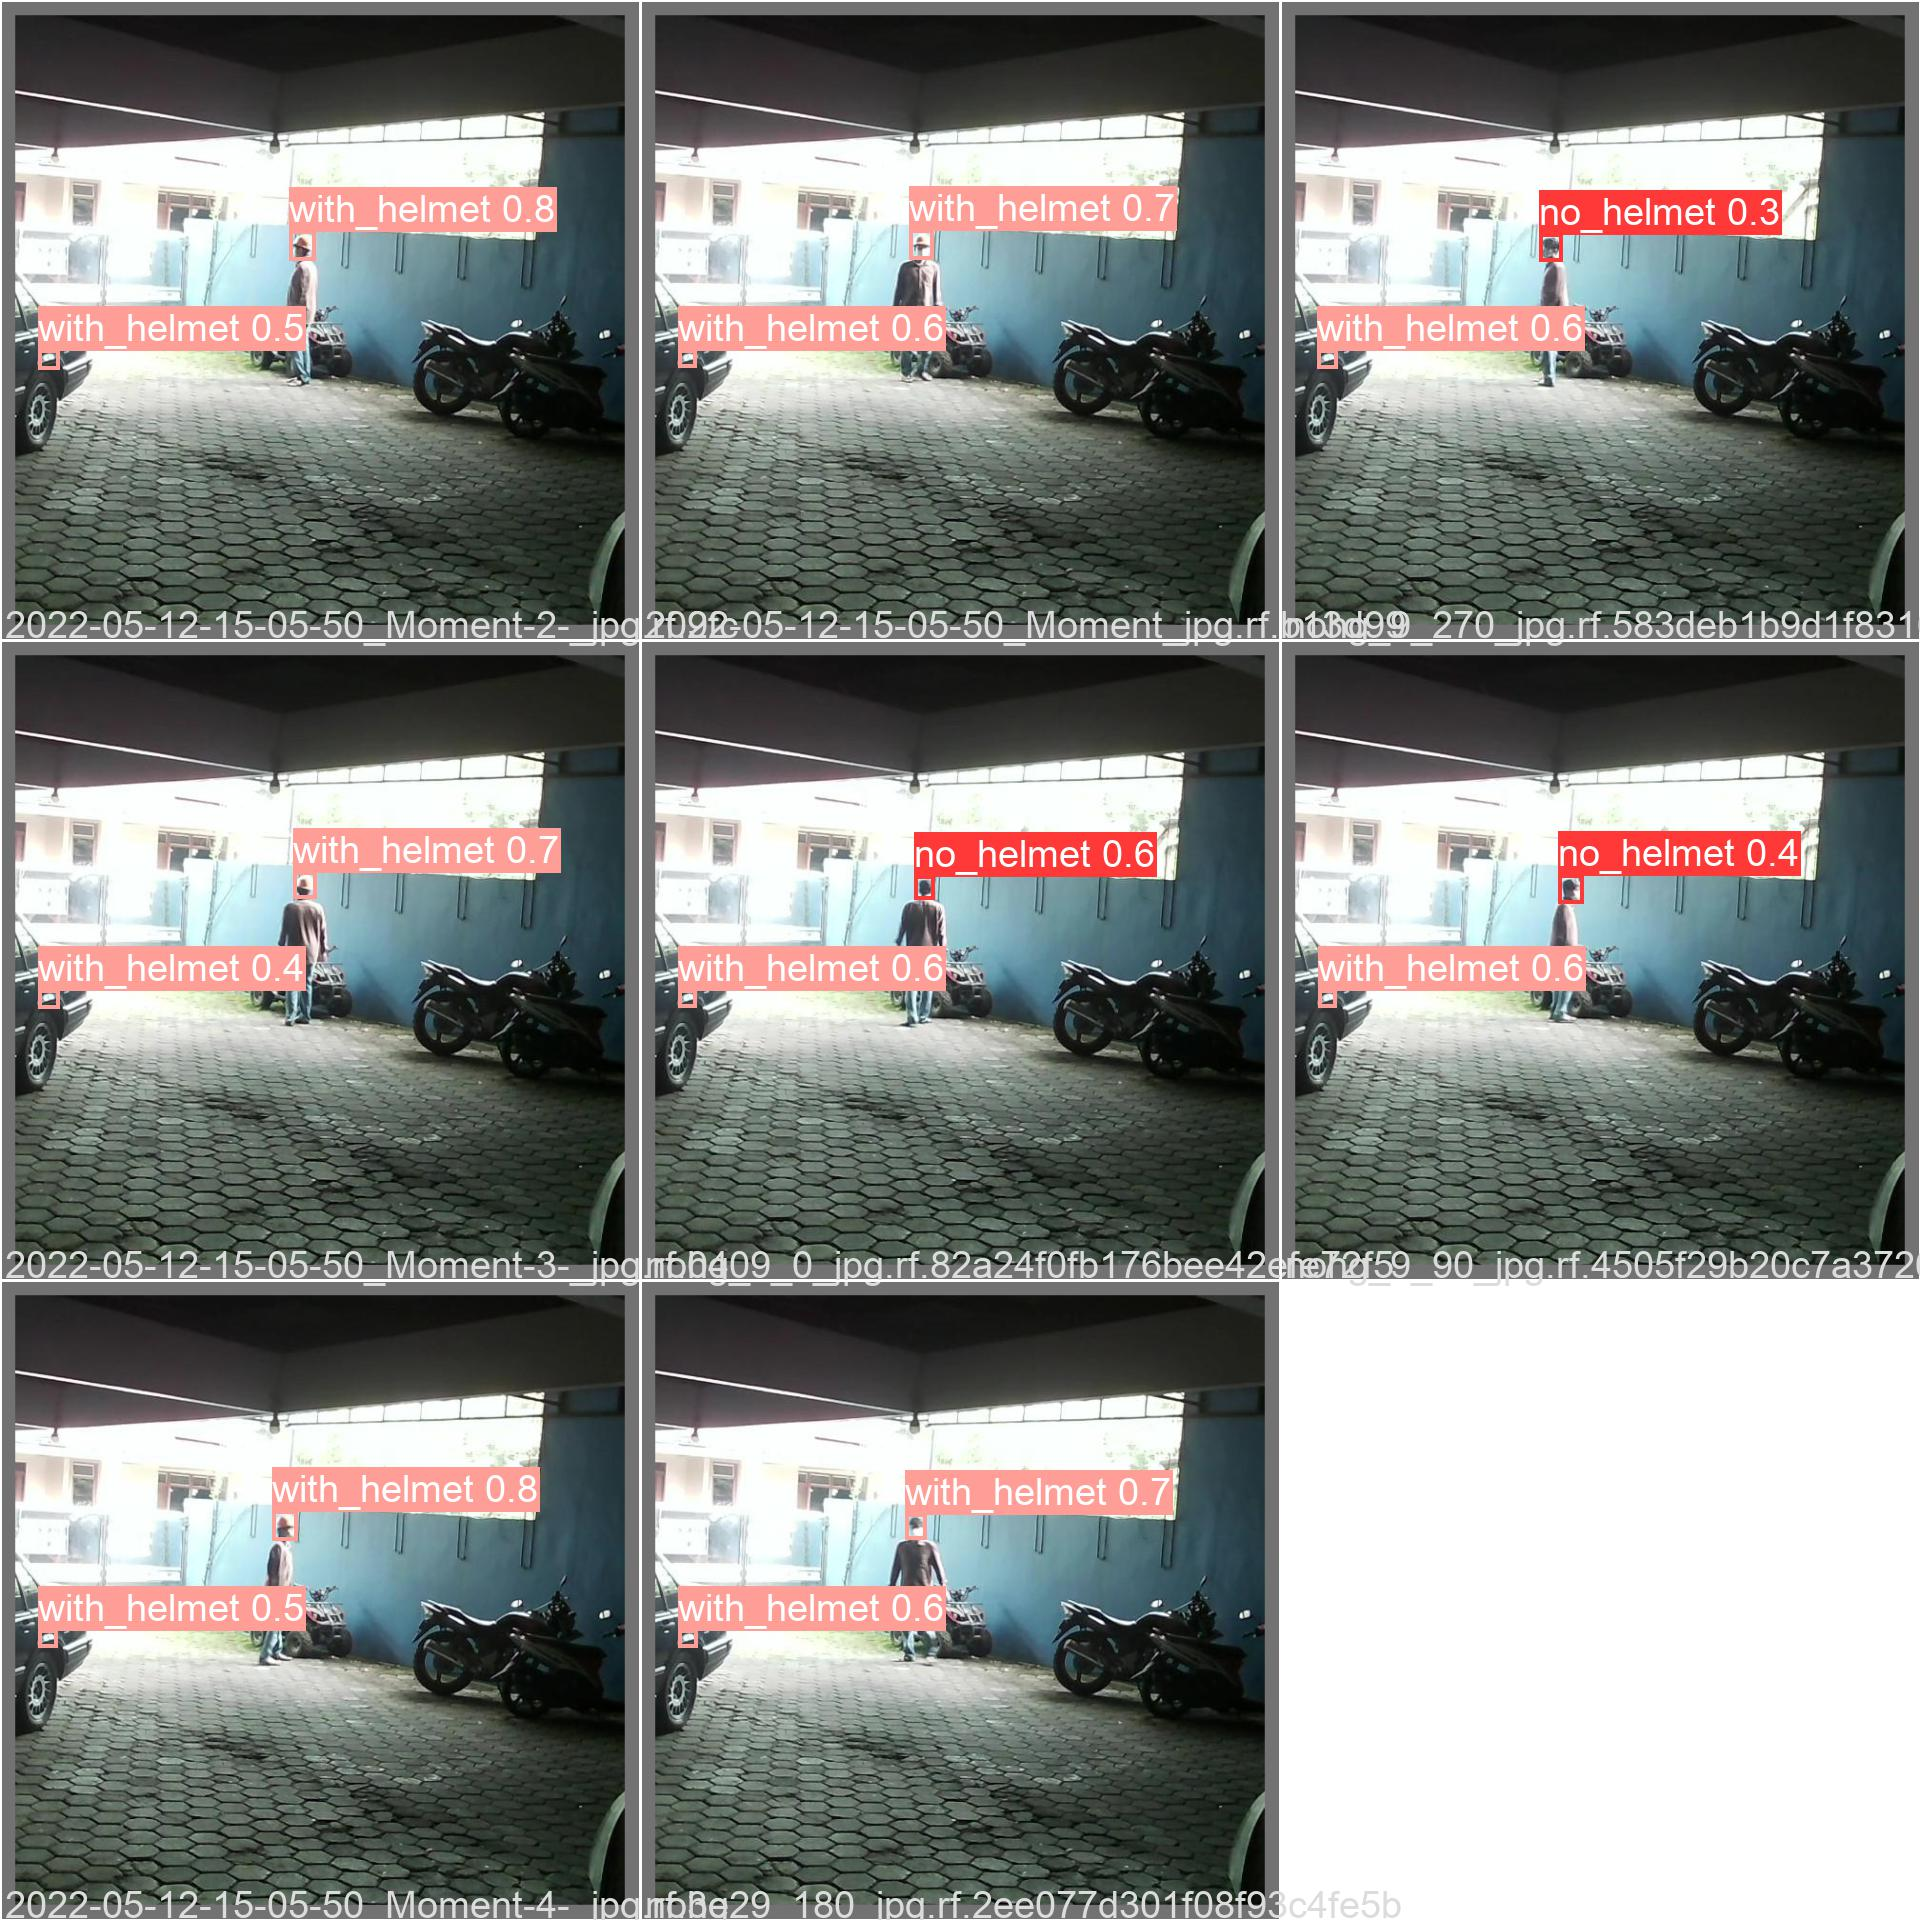
\includegraphics[width=0.3\textwidth]{gambar/BerdasarkanJarak_v2/val_hedec_pretrain_M/Jarak9/val_batch0_pred.jpg}
    \caption{Hasil Prediksi Untuk Bobot "hedec\_pretrain\_M" Pada Perbedaan Jarak}
    \label{fig:valjarak_sample_hedec_pretrain_M}  
  \end{figure}

   
  \item \textbf{hedec\_pretrain\_L}
  
  \par Pada pengujian menggunakan bobot "hedec\_pretrain\_L" pada perbedaan jarak, bobot ini memiliki hasil pengujian
  paling baik diantara bobot yang di\emph{train} menggunakan \emph{Pretrained Weights} dari YOLOv5 dimana untuk \emph{precision, recall,} dan \emph{mAP} berada di atas 0.9 untuk semua jarak
  dan kelas. Hasil validasi dapat dilihat pada Tabel~\ref{tb:hasiljarak_hedec_pretrain_L}.

  \par Seperti yang bisa dilihat dari Gambar~\ref{fig:grafvaljarak_hedec_pretrain_L}, hanya terjadi sedikit penurunan presisi
  pada jarak 1.3 meter untuk kelas "with\_helmet". Selain itu semua konstan di atas angka 0.98.


  \begin{longtable}{|l|l|l|l|l|} 
    \caption{Hasil Validasi Perbedaan Jarak Pada \textbf{"hedec\_pretrain\_L"}}
    \label{tb:hasiljarak_hedec_pretrain_L}\\
    \hline
    Jarak     & class        & precision & recall & mAP    \\ 
    \hline
    1.3 meter & all          & 0.984     & 1      & 0.995  \\
    2.6 meter & all          & 0.987     & 1      & 0.995  \\
    4 meter   & all          & 0.988     & 1      & 0.995  \\
    5.3 meter & all          & 0.988     & 1      & 0.995  \\
    6.7 meter & all          & 0.989     & 1      & 0.995  \\
    9 meter   & all          & 0.988     & 1      & 0.995  \\
    1.3 meter & no\_helmet   & 0.992     & 1      & 0.995  \\
    2.6 meter & no\_helmet   & 0.99      & 1      & 0.995  \\
    4 meter   & no\_helmet   & 0.989     & 1      & 0.995  \\
    5.3 meter & no\_helmet   & 0.99      & 1      & 0.995  \\
    6.7 meter & no\_helmet   & 0.99      & 1      & 0.995  \\
    9 meter   & no\_helmet   & 0.987     & 1      & 0.995  \\
    1.3 meter & with\_helmet & 0.975     & 1      & 0.995  \\
    2.6 meter & with\_helmet & 0.985     & 1      & 0.995  \\
    4 meter   & with\_helmet & 0.988     & 1      & 0.995  \\
    5.3 meter & with\_helmet & 0.985     & 1      & 0.995  \\
    6.7 meter & with\_helmet & 0.988     & 1      & 0.995  \\
    9 meter   & with\_helmet & 0.988     & 1      & 0.995  \\
    \hline
  \end{longtable}

  \begin{figure} [h!]
    \centering
    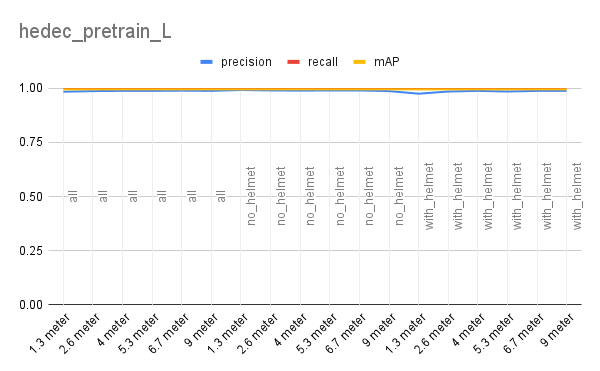
\includegraphics[width=1\textwidth]{gambar/BerdasarkanJarak/hedec_pretrain_L.png}
    \caption{Grafik \emph{Precision, Recall, mAP} untuk \textbf{"hedec\_pretrain\_L"} Pada Jarak 1.3 meter Hingga 9 meter}
    \label{fig:grafvaljarak_hedec_pretrain_L}  
  \end{figure}

  \begin{figure} [h!]
    \centering
    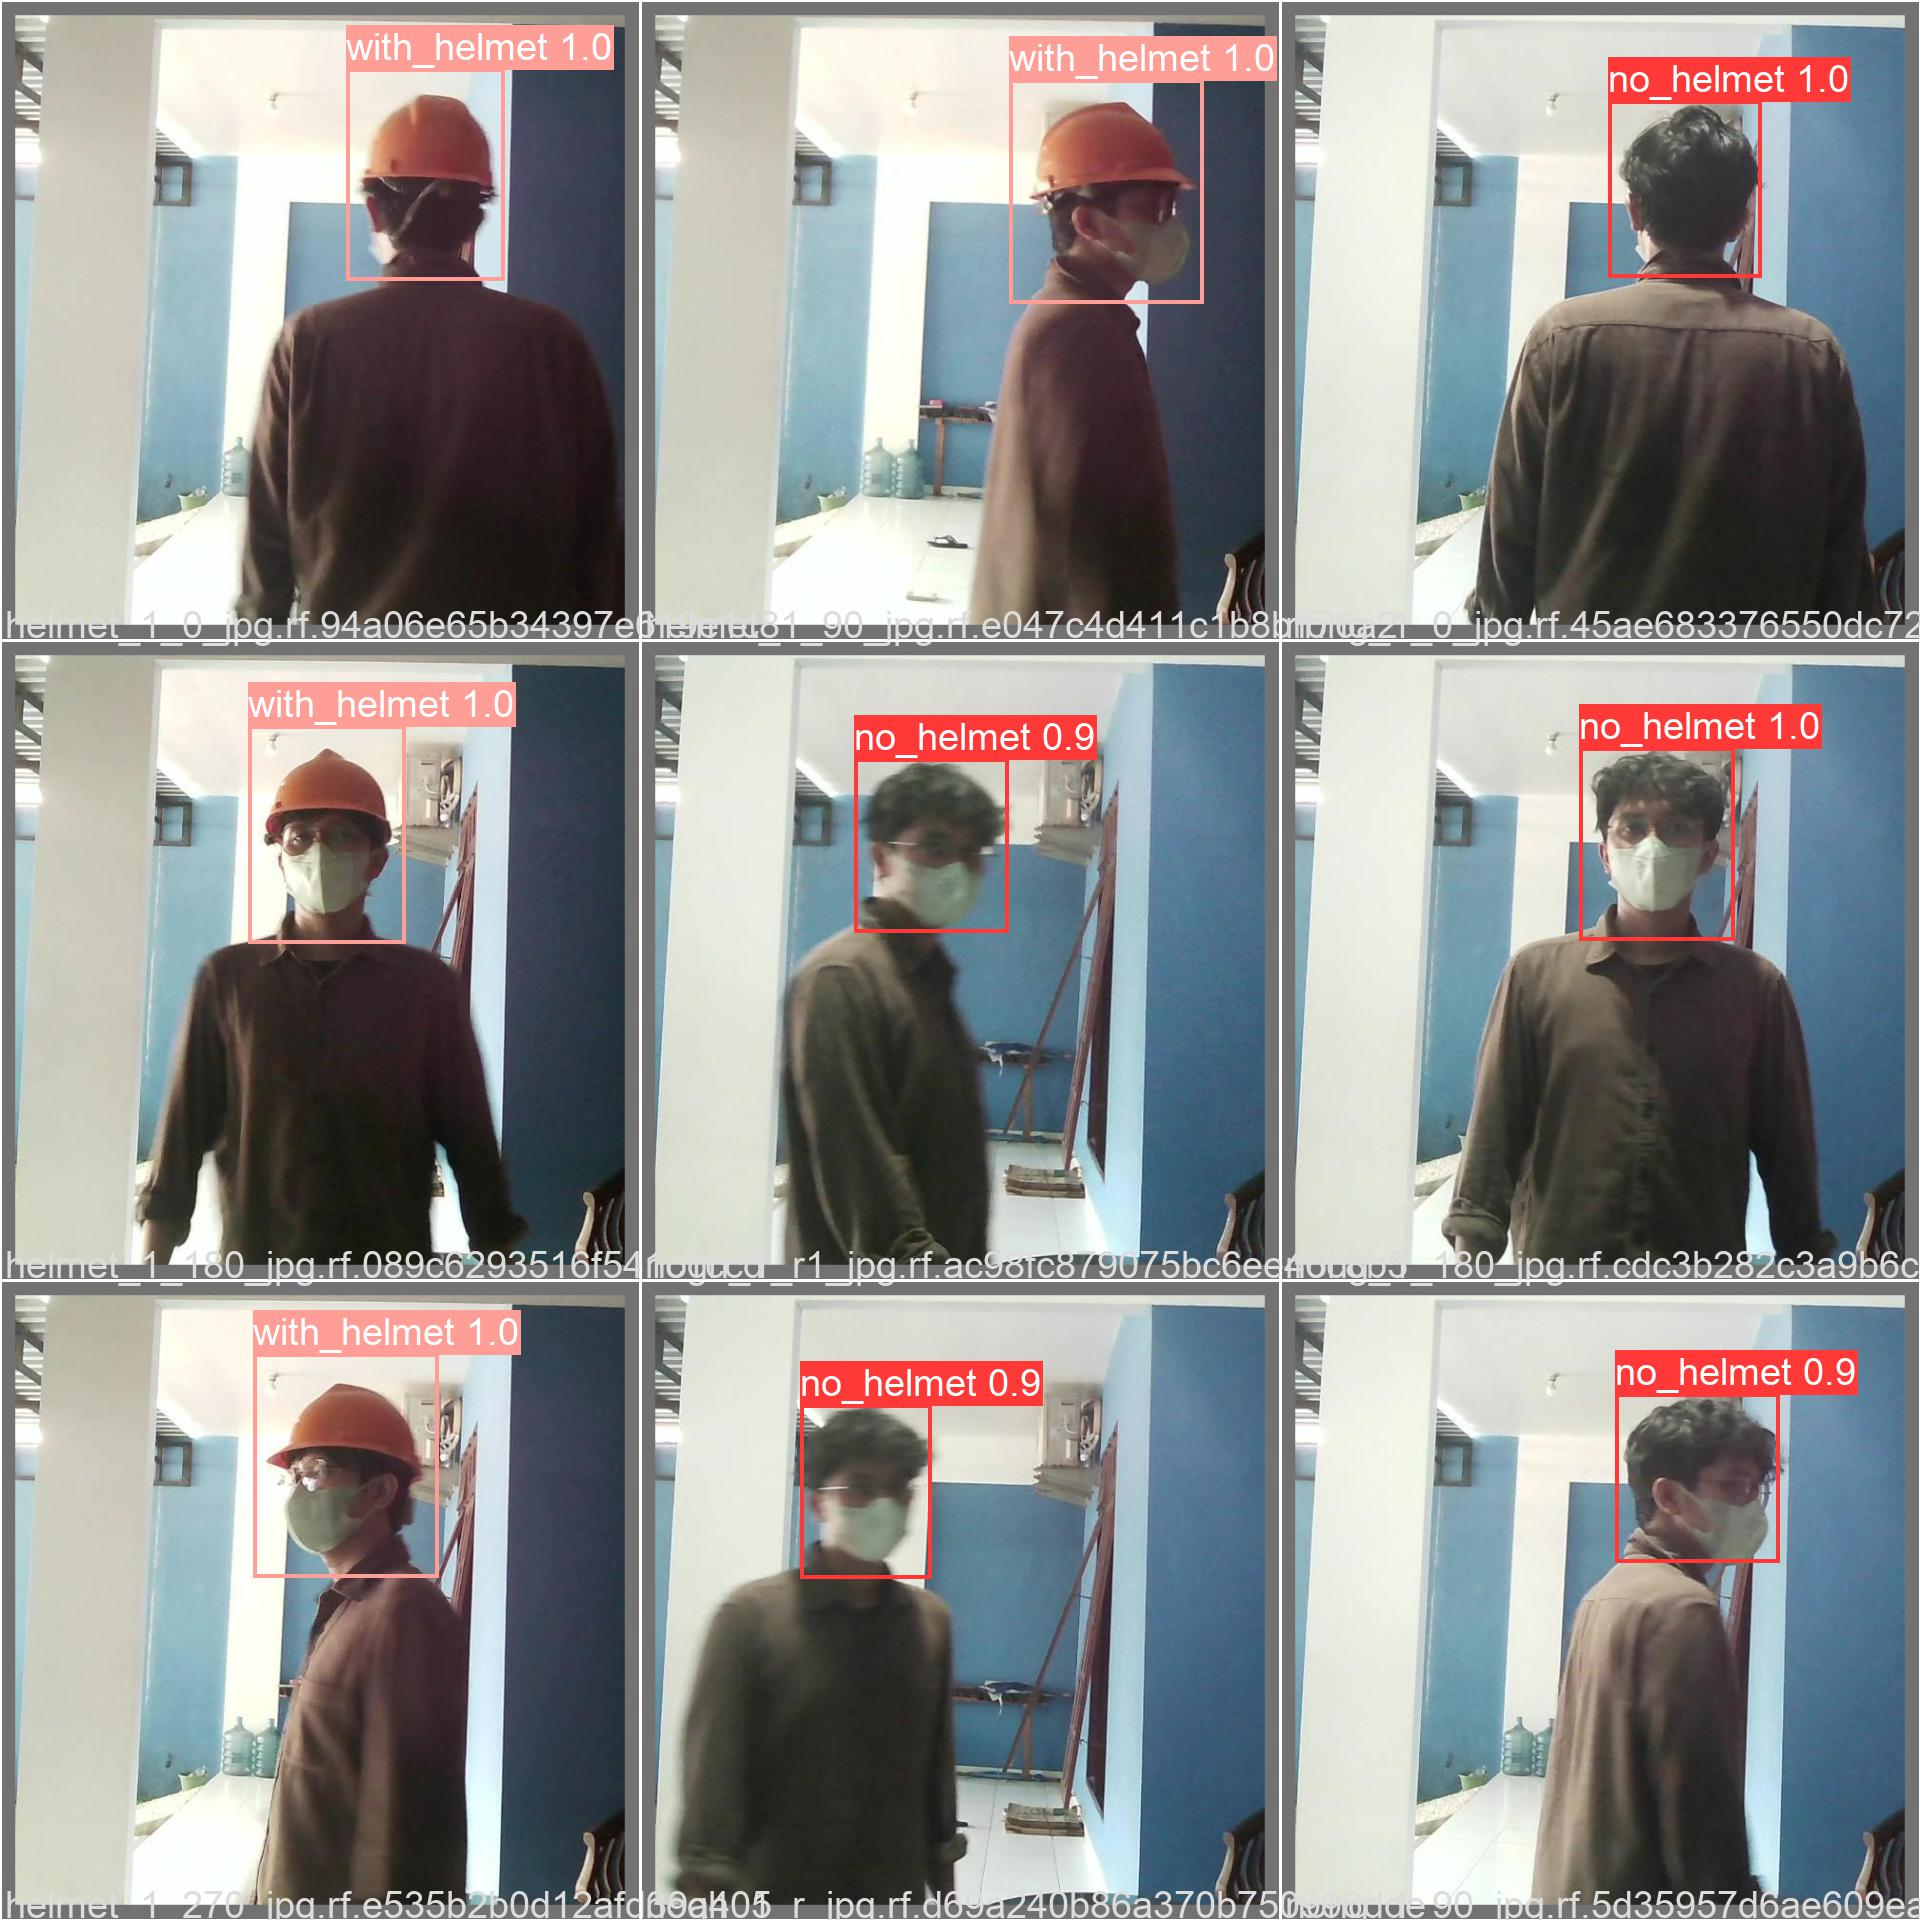
\includegraphics[width=0.3\textwidth]{gambar/BerdasarkanJarak_v2/val_hedec_pretrain_L/Jarak1_3/val_batch0_pred.jpg}
    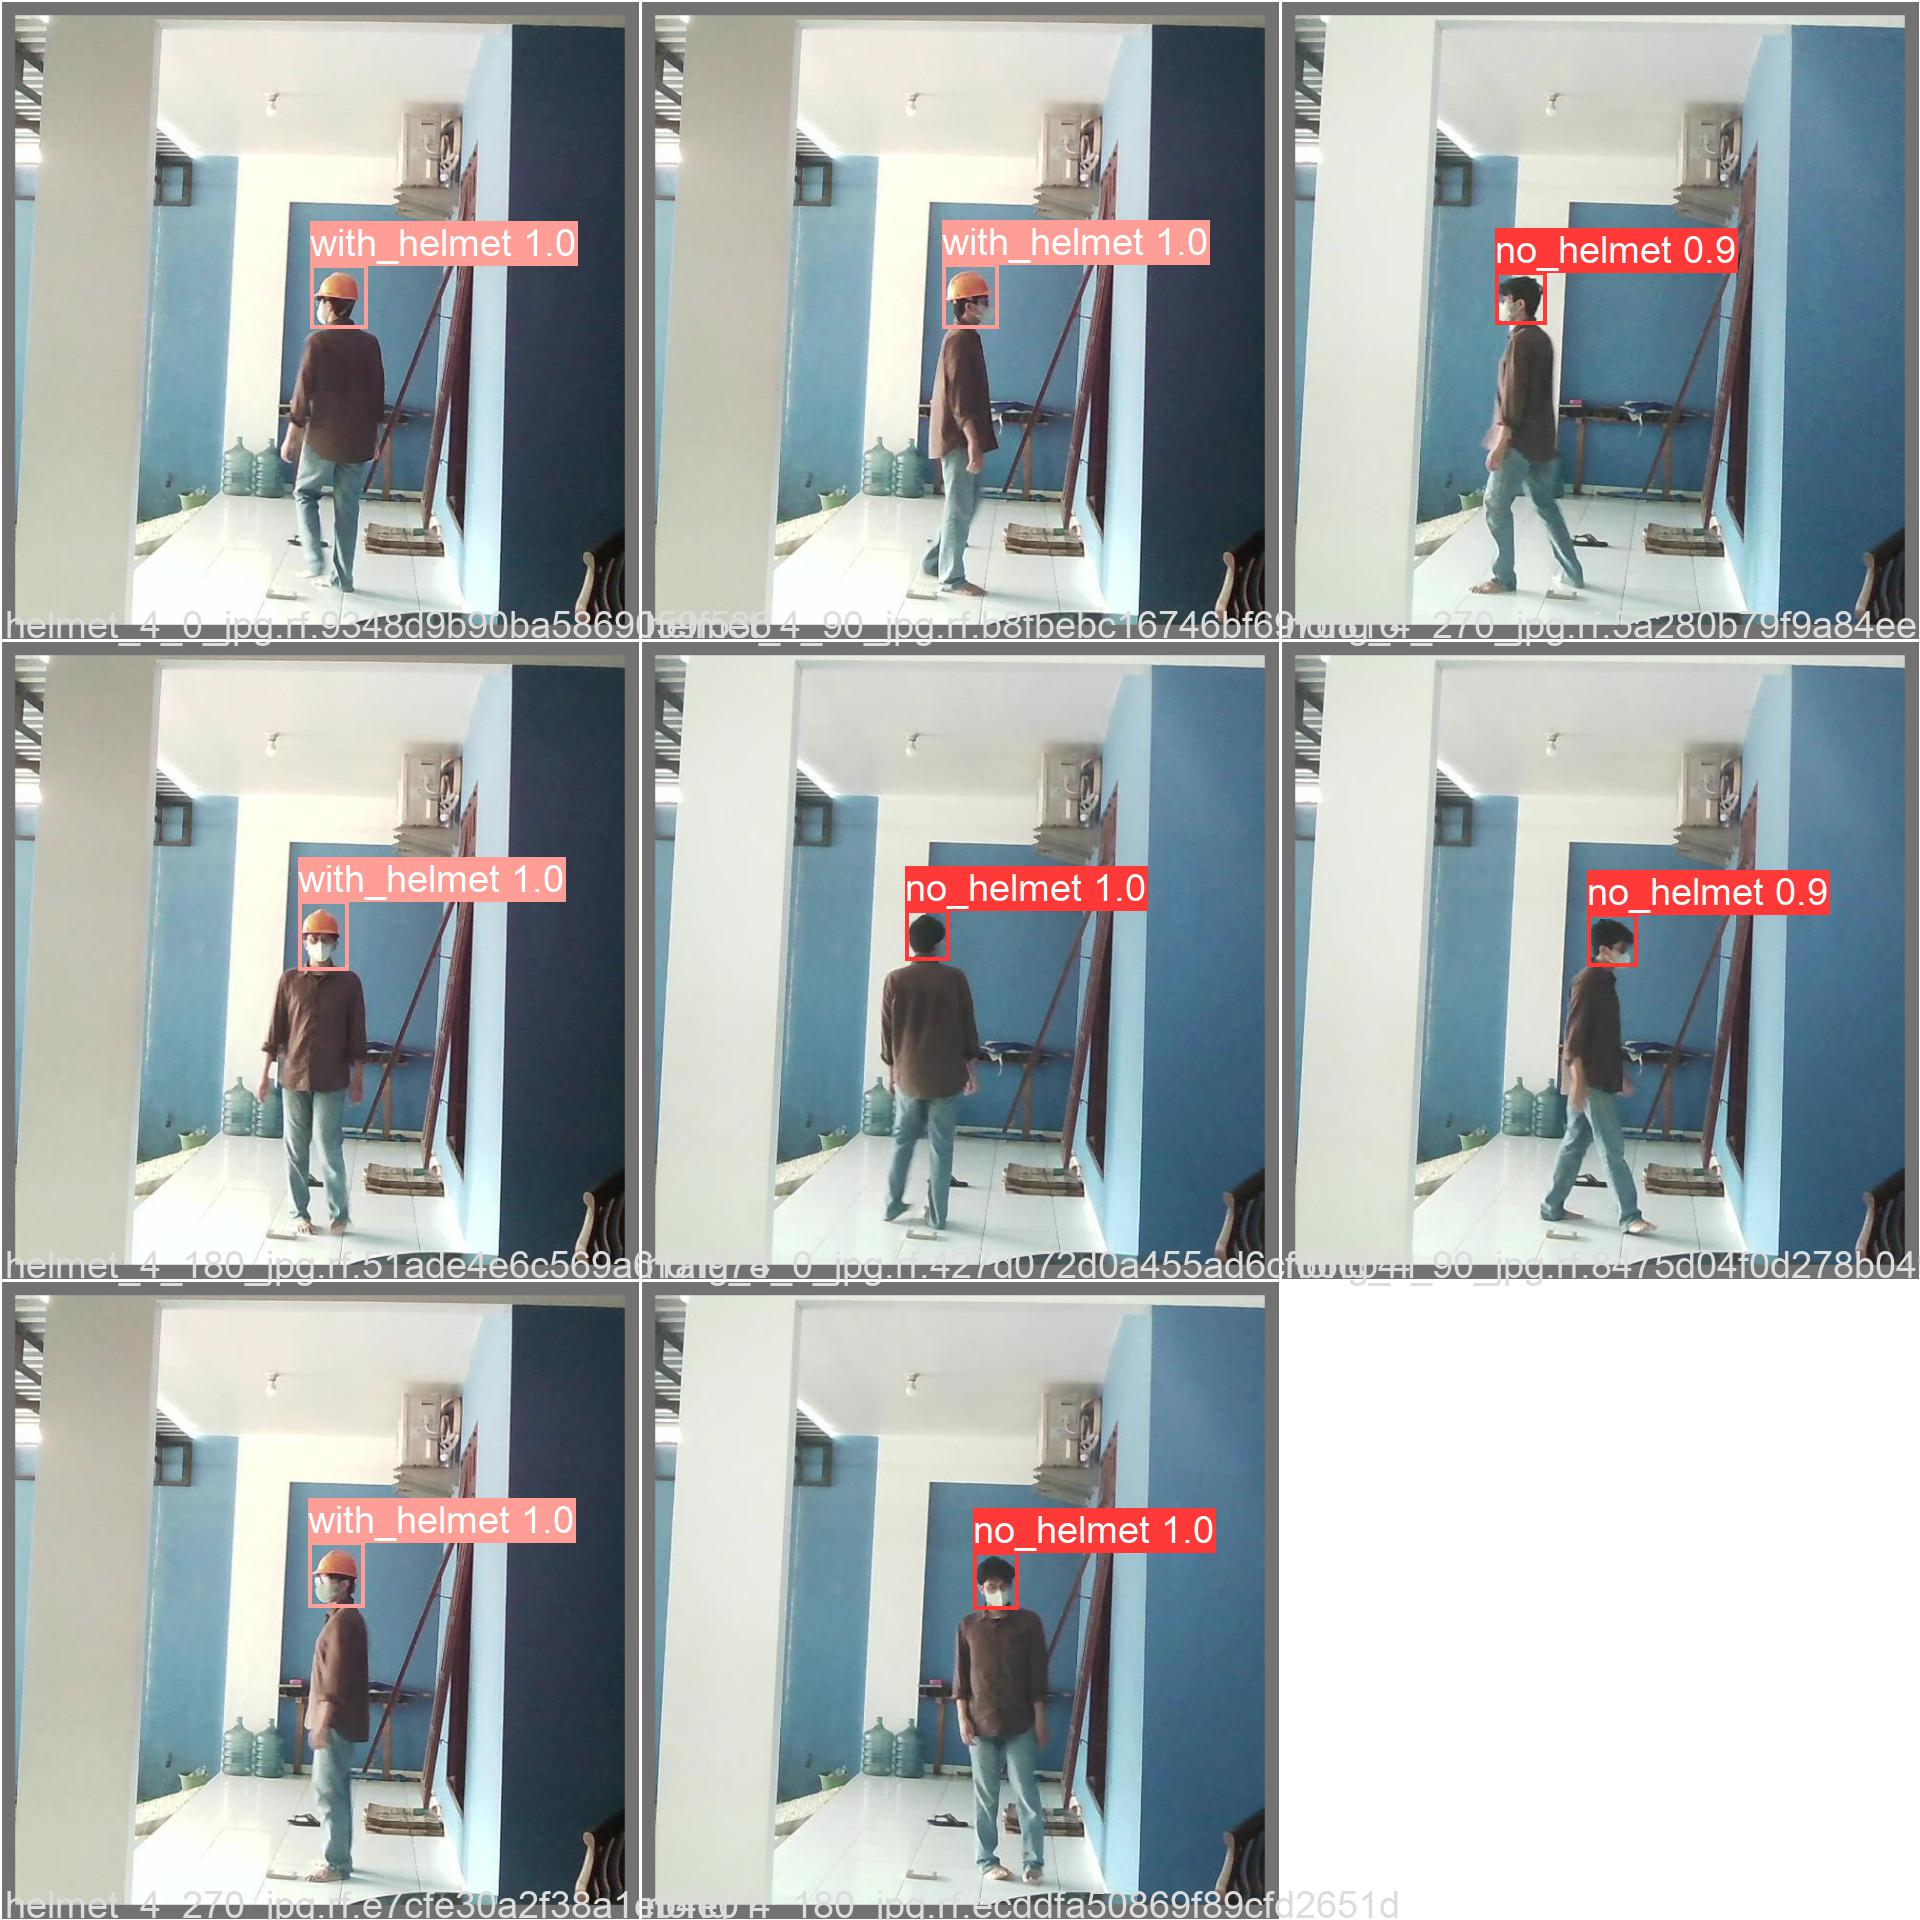
\includegraphics[width=0.3\textwidth]{gambar/BerdasarkanJarak_v2/val_hedec_pretrain_L/Jarak5_3/val_batch0_pred.jpg}
    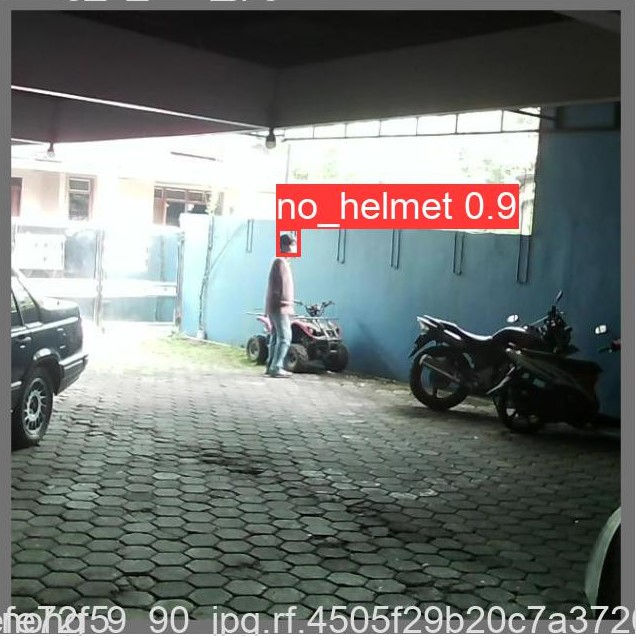
\includegraphics[width=0.3\textwidth]{gambar/BerdasarkanJarak_v2/val_hedec_pretrain_L/Jarak9/val_batch0_pred.jpg}
    \caption{Hasil Prediksi Untuk Bobot "hedec\_pretrain\_L" Pada Perbedaan Jarak}
    \label{fig:valjarak_sample_hedec_pretrain_L}  
  \end{figure}

\end{enumerate}


\newpage
\subsection{Pengujian Jarak dengan \emph{Pure Weight}}
\label{subsec:ujijarak_pureweight}

\par Bagian ini memaparkan pengujian menggunakan bobot hasil \emph{training} tanpa menggunakan \emph{Pretrained Weights}
dari repo YOLOv5 yang selanjutnya disebut sebagai "hedec\_pure". 

\begin{enumerate}
  \item \textbf{hedec\_pure\_N}
  \par Pada bagian dipaparkan hasil pengujian dari bobot "hedec\_pure\_N" yang merupakan bobot hasil \emph{training}
  yang tidak menggunakan \emph{Pretrained Weights} dari repository YOLOv5 tetapi konfigurasinya menyerupai konfigurasi
  varian \emph{Pretrained Weights} varian YOLOv5n. Seperti yang ditunjukkan pada Gambar~\ref{fig:grafvaljarak_hedec_pure_N}
  , untuk semua kelas memiliki nilai \emph{precision} di atas 0.8 untuk semua jarak. Tetapi untuk \emph{recall} pada jarak 1.3 meter
  untuk kelas "no\_helmet" memiliki nilai 0.6 dimana terdapat kegagalan memprediksi kelas "no\_helmet" dan prediksi lokasi yang
  kurang akurat. Tabel Hasil Validasi bobot "hedec\_pure\_N" bisa dilihat pada Tabel~\ref{tb:hasiljarak_hedec_pure_N}.

  \begin{figure} [h!]
    \centering
    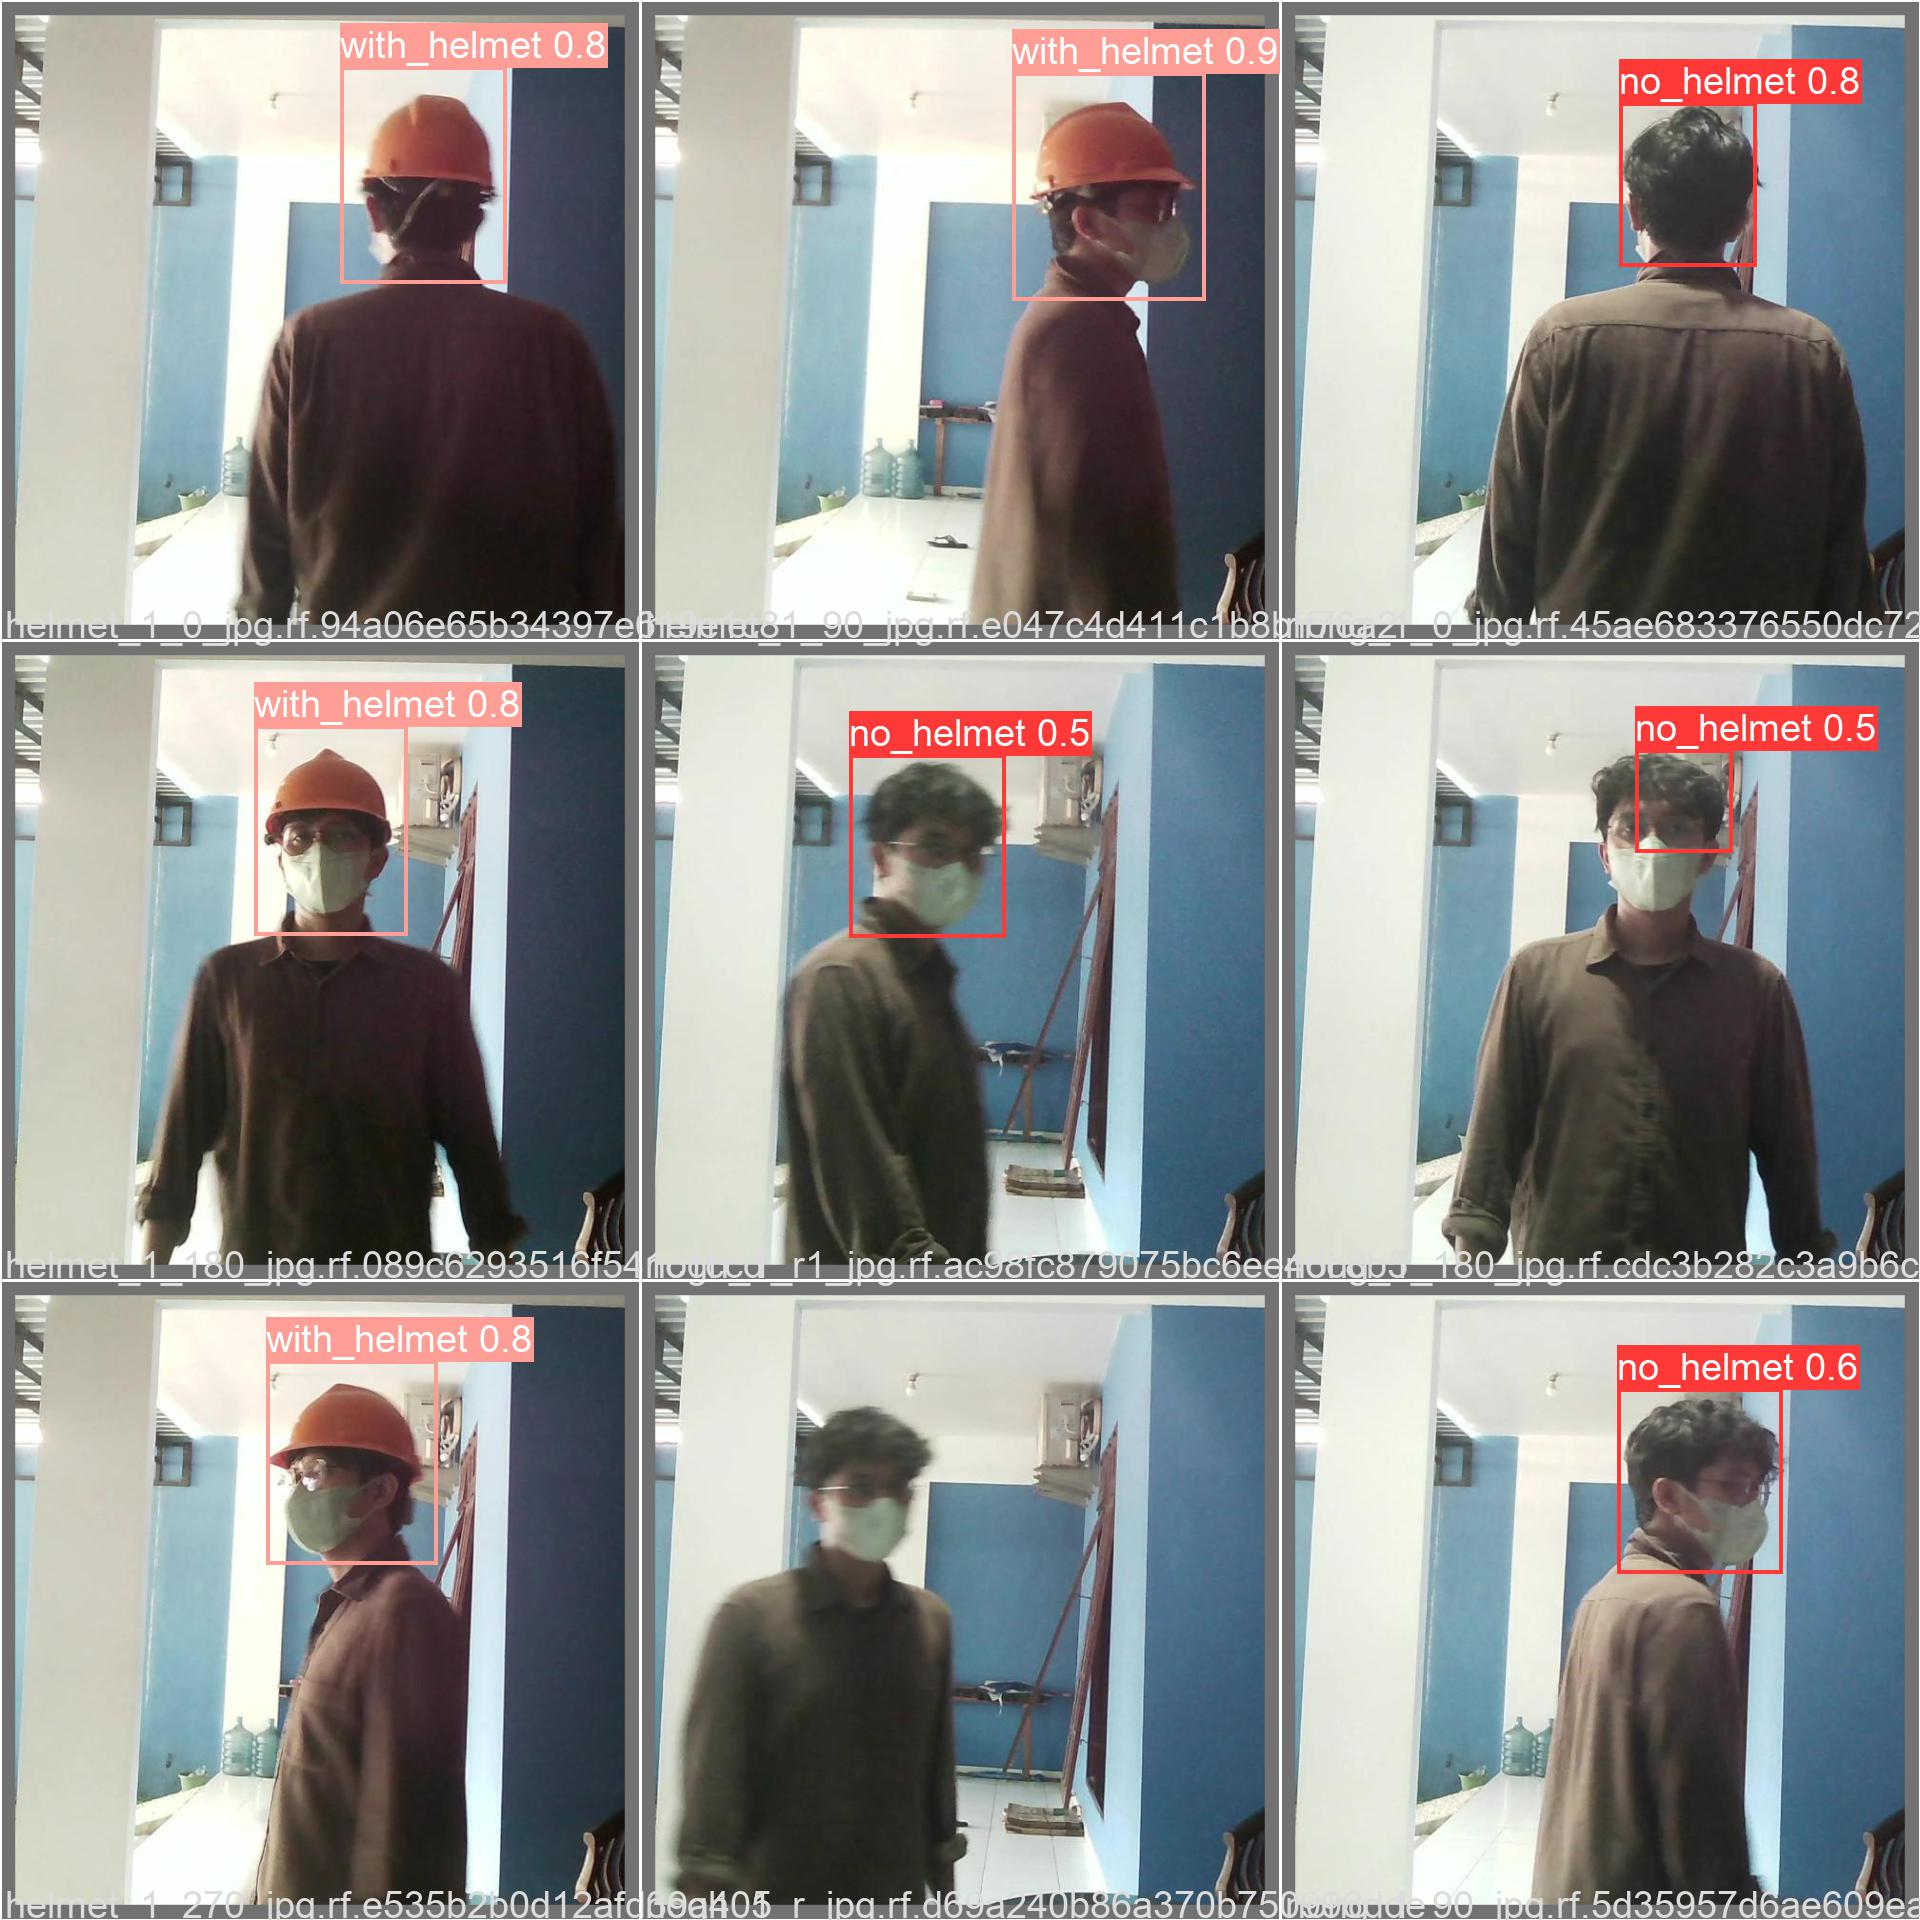
\includegraphics[width=0.3\textwidth]{gambar/BerdasarkanJarak_v2/val_hedec_pure_N/Jarak1_3/val_batch0_pred.jpg}
    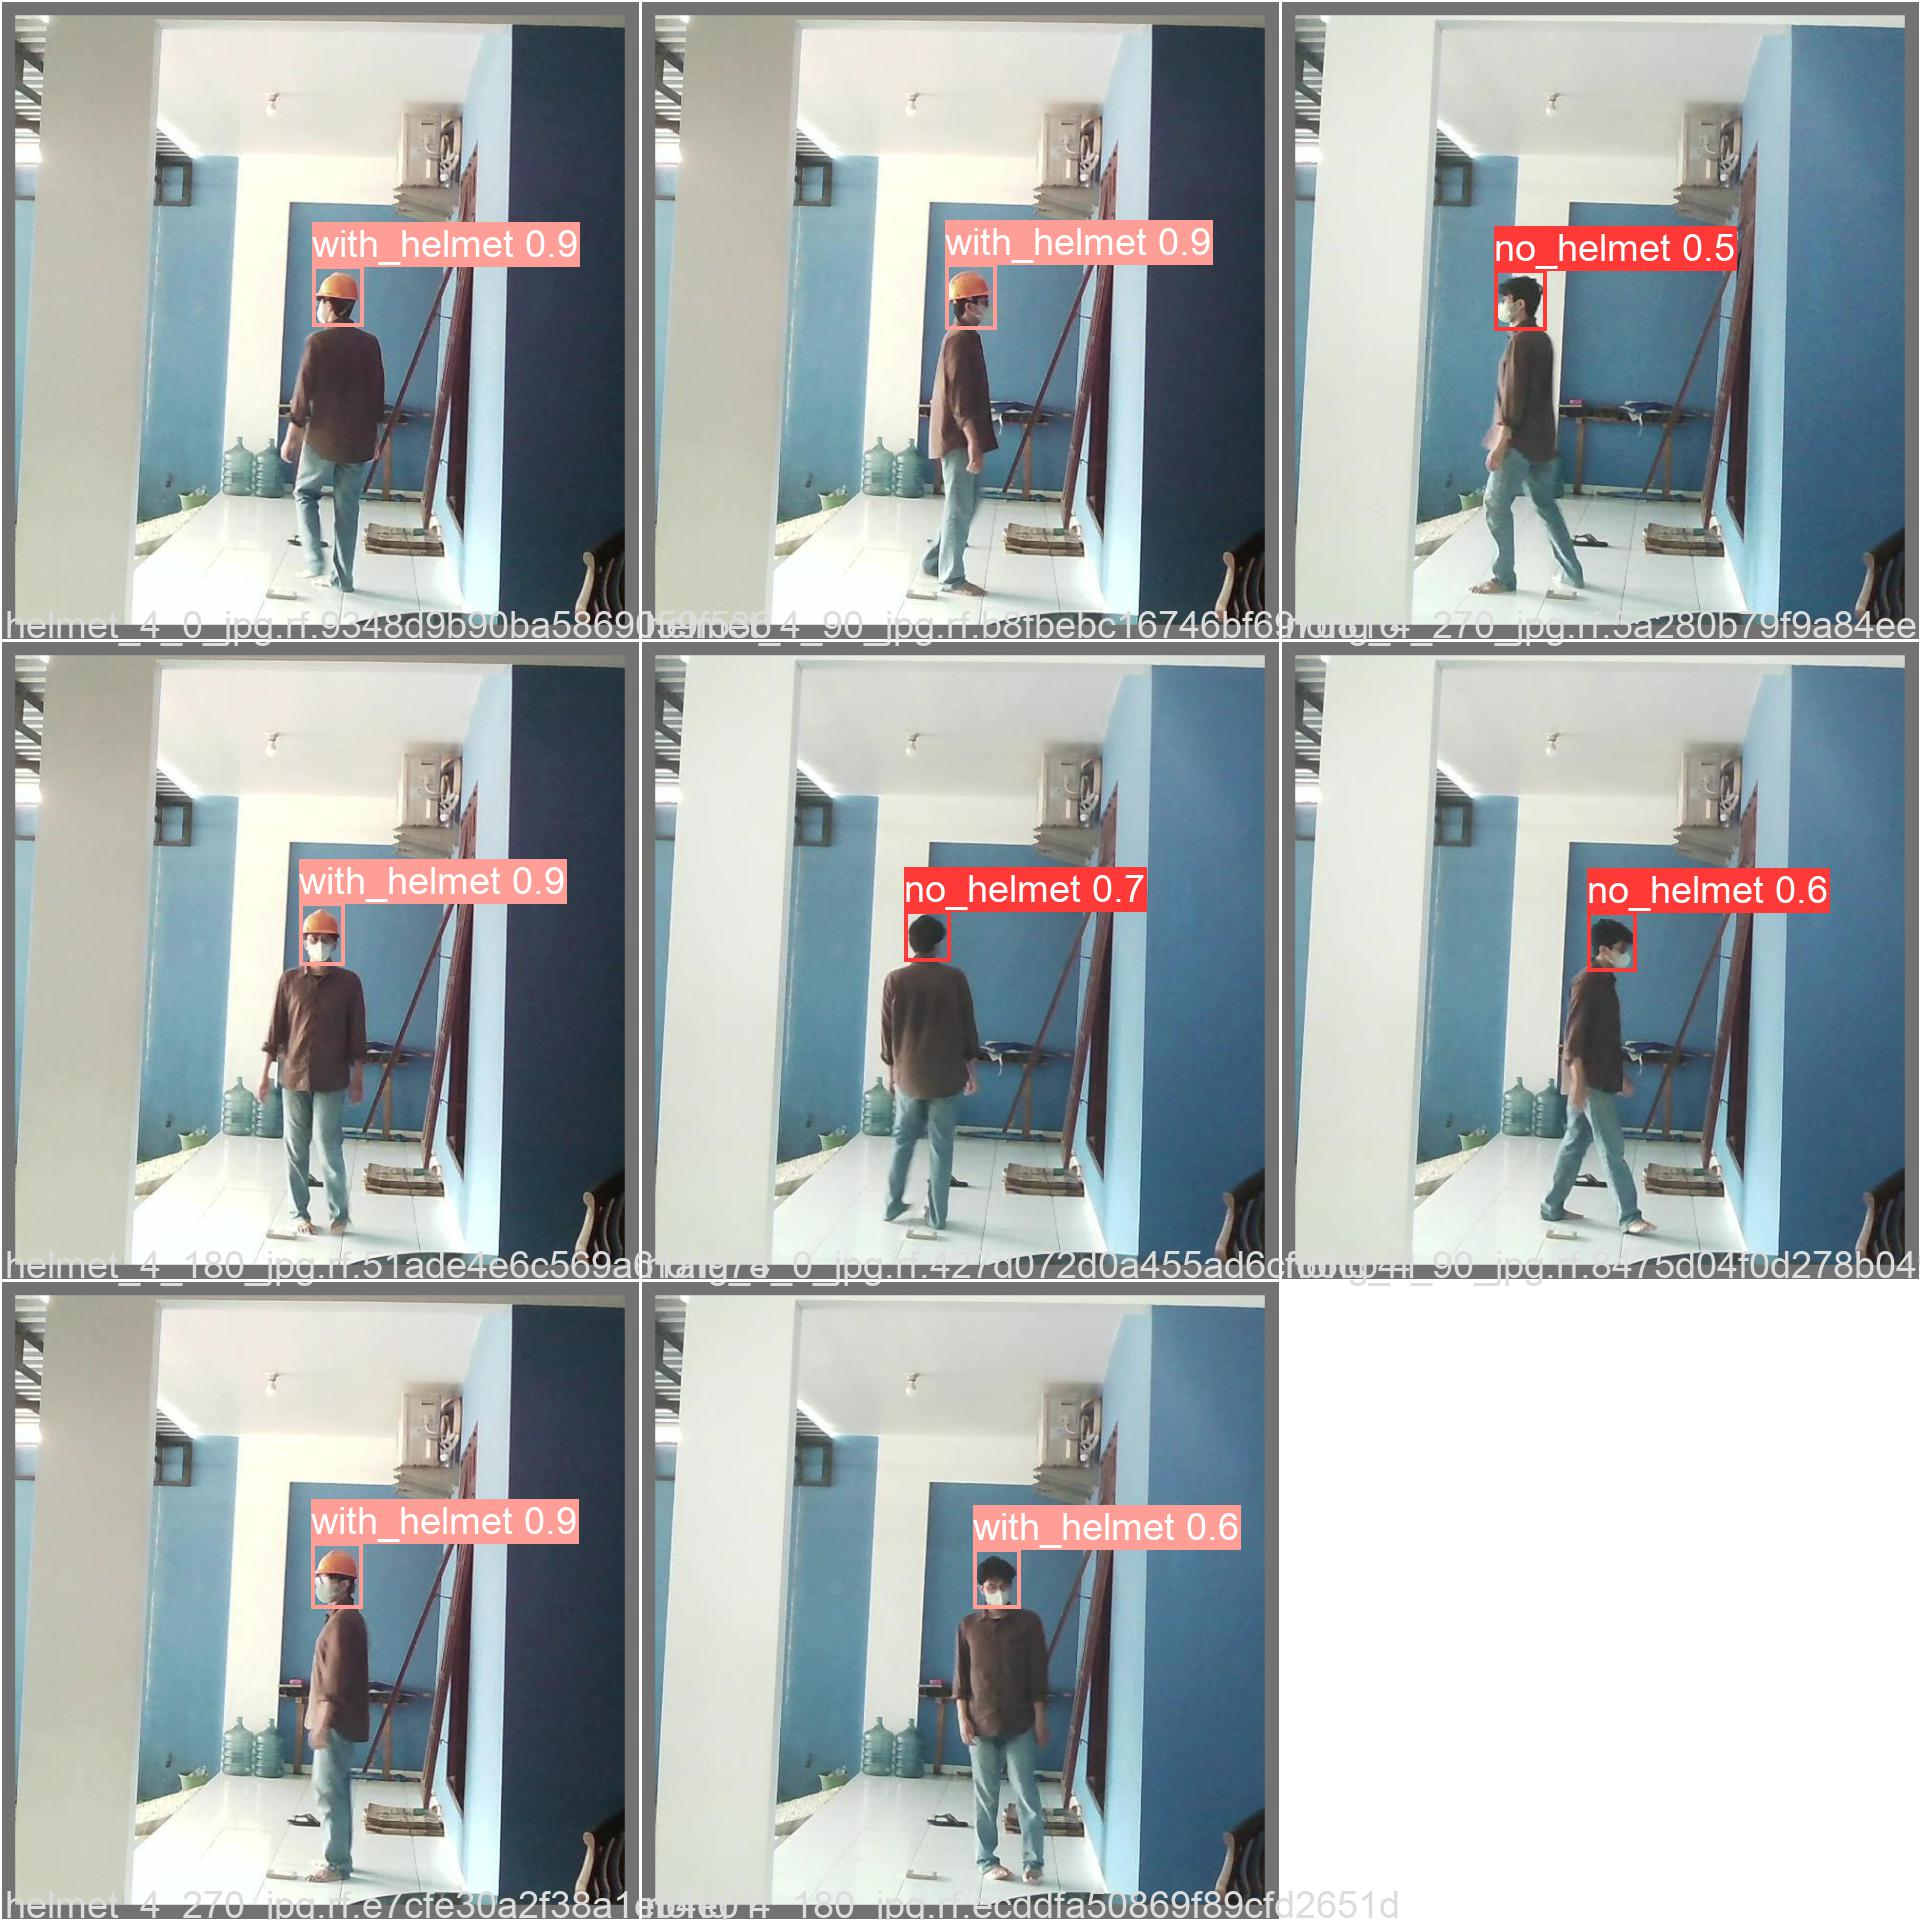
\includegraphics[width=0.3\textwidth]{gambar/BerdasarkanJarak_v2/val_hedec_pure_N/Jarak5_3/val_batch0_pred.jpg}
    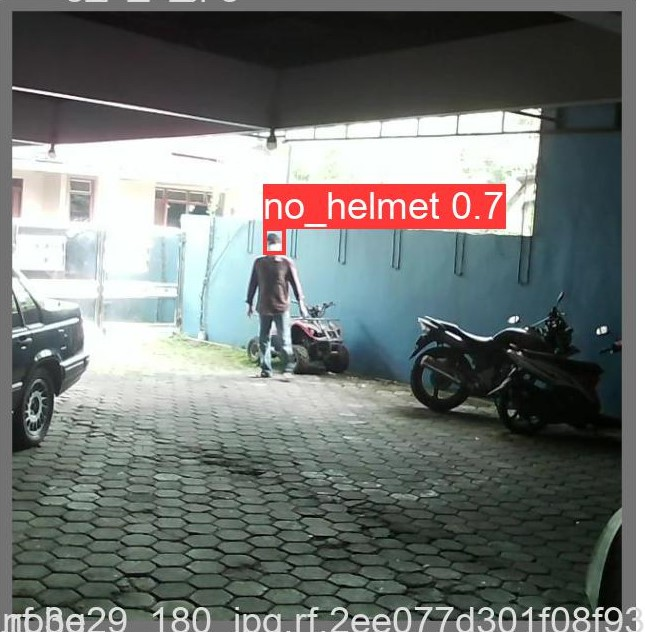
\includegraphics[width=0.3\textwidth]{gambar/BerdasarkanJarak_v2/val_hedec_pure_N/Jarak9/val_batch0_pred.jpg}
    \caption{Hasil Prediksi Untuk Bobot "hedec\_pure\_N" Pada Perbedaan Jarak}
    \label{fig:valjarak_sample_hedec_pure_N}  
  \end{figure}

  \begin{longtable}{|l|l|l|l|l|} 
    \caption{Hasil Validasi Perbedaan Jarak Pada \textbf{"hedec\_pure\_N"}}
    \label{tb:hasiljarak_hedec_pure_N}\\
    \hline
      Jarak     & class        & precision & recall & mAP    \\ 
      \hline
      1.3 meter & all          & 0.889     & 0.8    & 0.903  \\
      2.6 meter & all          & 0.971     & 1      & 0.995  \\
      4 meter   & all          & 0.904     & 0.986  & 0.995  \\
      5.3 meter & all          & 0.847     & 0.989  & 0.995  \\
      6.7 meter & all          & 0.949     & 1      & 0.995  \\
      9 meter   & all          & 0.92      & 1      & 0.995  \\
      1.3 meter & no\_helmet   & 0.876     & 0.6    & 0.812  \\
      2.6 meter & no\_helmet   & 0.991     & 1      & 0.995  \\
      4 meter   & no\_helmet   & 1         & 0.971  & 0.995  \\
      5.3 meter & no\_helmet   & 1         & 0.977  & 0.995  \\
      6.7 meter & no\_helmet   & 0.997     & 1      & 0.995  \\
      9 meter   & no\_helmet   & 0.979     & 1      & 0.995  \\
      1.3 meter & with\_helmet & 0.902     & 1      & 0.995  \\
      2.6 meter & with\_helmet & 0.952     & 1      & 0.995  \\
      4 meter   & with\_helmet & 0.808     & 1      & 0.995  \\
      5.3 meter & with\_helmet & 0.694     & 1      & 0.995  \\
      6.7 meter & with\_helmet & 0.901     & 1      & 0.995  \\
      9 meter   & with\_helmet & 0.861     & 1      & 0.995  \\
      \hline
  \end{longtable}

  \begin{figure} [h!]
    \centering
    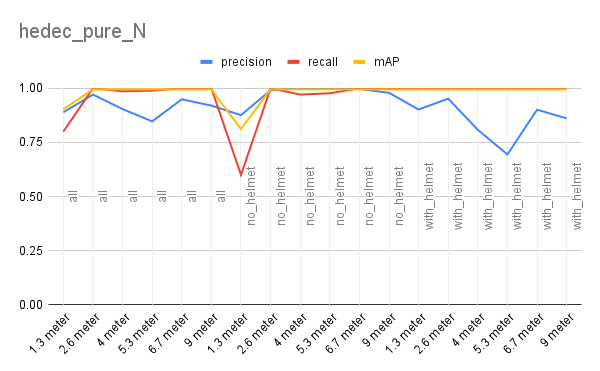
\includegraphics[width=1\textwidth]{gambar/BerdasarkanJarak/hedec_pure_N.png}
    \caption{Grafik \emph{Precision, Recall, mAP} untuk \textbf{"hedec\_pure\_N"} Pada Jarak 1.3 meter Hingga 9 meter}
    \label{fig:grafvaljarak_hedec_pure_N}  
  \end{figure}

  

  \FloatBarrier


  \item \textbf{hedec\_pure\_S}
  
  \par Pada pengujian pada jarak berbeda dari 1.3 meter hingga 9 meter untuk bobot "hedec\_pure\_S" yang merupakan bobot hasil \emph{training}
  yang tidak menggunakan \emph{Pretrained Weights} dari repository YOLOv5 tetapi konfigurasinya menyerupai konfigurasi
  varian \emph{Pretrained Weights} varian YOLOv5s ini ditemukan beberapa hal. Seperti yang bisa dilihat pada Gambar~\ref{fig:grafvaljarak_hedec_pure_S},
  pada jarak 1.3 meter memiliki nilai yang rendah untuk \emph{precision, recall} dan juga nilai mAP nya dimana untuk kelas "no\_helmet" didapati kesalahan prediksi. Lalu mulai dari
  jarak 2.6 meter hingga 6.7 meter mengalami kenaikan. Tetapi pada jarak 9 meter, \emph{precision} untuk kelas "with\_helmet"
  mengalami penurunan karena ada kelas "no\_helmet" yang terdeteksi sebagai "with\_helmet". Tabel untuk hasil validasi dari "hedec\_pure\_N" bisa dilihat
  pada Tabel~\ref{tb:hasiljarak_hedec_pure_S}.
  
  \begin{longtable}{|l|l|l|l|l|} 
    \caption{Hasil Validasi Perbedaan Jarak Pada \textbf{"hedec\_pure\_S"}}
    \label{tb:hasiljarak_hedec_pure_S}\\
    \hline
    Jarak     & class        & precision & recall & mAP    \\ 
    \hline
    1.3 meter & all          & 0.846     & 0.8    & 0.891  \\
    2.6 meter & all          & 0.978     & 1      & 0.995  \\
    4 meter   & all          & 0.959     & 1      & 0.995  \\
    5.3 meter & all          & 0.891     & 1      & 0.995  \\
    6.7 meter & all          & 0.948     & 1      & 0.995  \\
    9 meter   & all          & 0.745     & 1      & 0.97   \\
    1.3 meter & no\_helmet   & 0.728     & 0.6    & 0.787  \\
    2.6 meter & no\_helmet   & 0.991     & 1      & 0.995  \\
    4 meter   & no\_helmet   & 0.987     & 1      & 0.995  \\
    5.3 meter & no\_helmet   & 0.985     & 1      & 0.995  \\
    6.7 meter & no\_helmet   & 0.994     & 1      & 0.995  \\
    9 meter   & no\_helmet   & 0.981     & 1      & 0.995  \\
    1.3 meter & with\_helmet & 0.964     & 1      & 0.995  \\
    2.6 meter & with\_helmet & 0.965     & 1      & 0.995  \\
    4 meter   & with\_helmet & 0.93      & 1      & 0.995  \\
    5.3 meter & with\_helmet & 0.797     & 1      & 0.995  \\
    6.7 meter & with\_helmet & 0.901     & 1      & 0.995  \\
    9 meter   & with\_helmet & 0.508     & 1      & 0.945  \\
    \hline
  \end{longtable}

  \begin{figure} [h!]
    \centering
    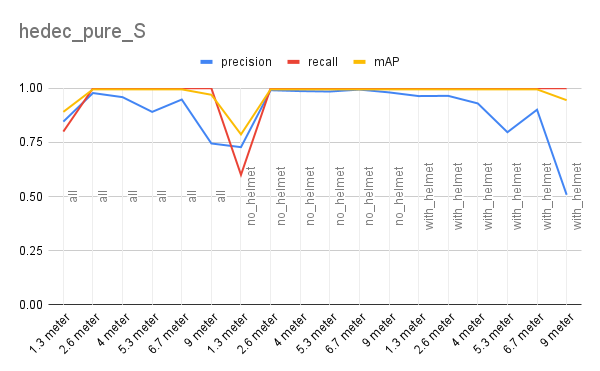
\includegraphics[width=1\textwidth]{gambar/BerdasarkanJarak/hedec_pure_S.png}
    \caption{Grafik \emph{Precision, Recall, mAP} untuk \textbf{"hedec\_pure\_S"} Pada Jarak 1.3 meter Hingga 9 meter}
    \label{fig:grafvaljarak_hedec_pure_S}  
  \end{figure}

  \begin{figure} [h!]
    \centering
    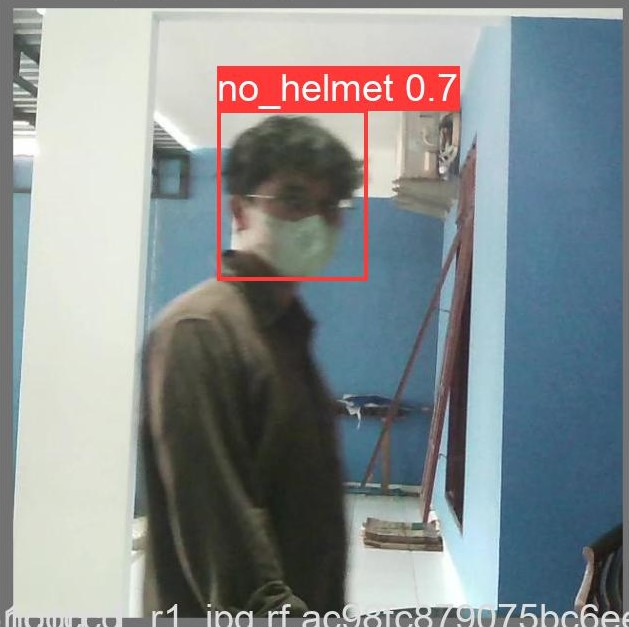
\includegraphics[width=0.3\textwidth]{gambar/BerdasarkanJarak_v2/val_hedec_pure_S/Jarak1_3/val_batch0_pred.jpg}
    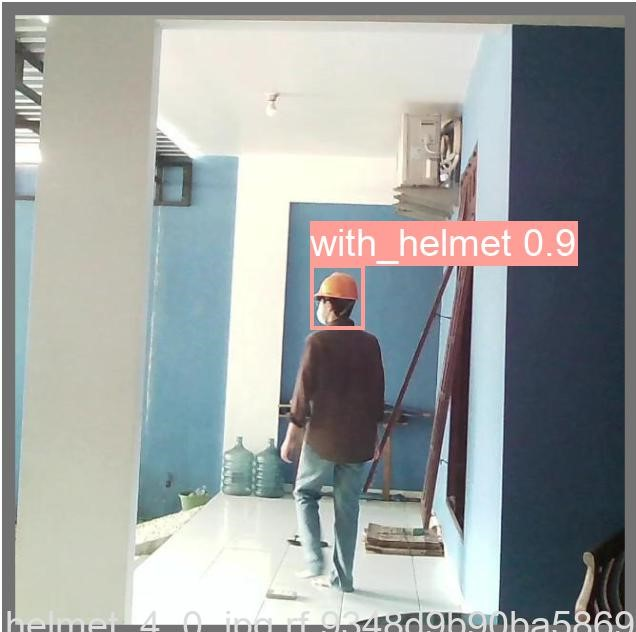
\includegraphics[width=0.3\textwidth]{gambar/BerdasarkanJarak_v2/val_hedec_pure_S/Jarak5_3/val_batch0_pred.jpg}
    \includegraphics[width=0.3\textwidth]{gambar/BerdasarkanJarak_v2/val_hedec_pure_S/Jarak9/val_batch0_pred.jpg}
    \caption{Hasil Prediksi Untuk Bobot "hedec\_pure\_S" Pada Perbedaan Jarak}
    \label{fig:valjarak_sample_hedec_pure_S}  
  \end{figure}

  \FloatBarrier

  \item \textbf{hedec\_pure\_M}
  
  \par Berikut merupakan hasil validasi pada pengujian prediksi dari jarak 1.3 meter hingga 9 meter untuk bobot "hedec\_pure\_M"
  yang konfigurasi nya menyerupai konfigurasi varian bobot YOLOv5m dari repo YOLOv5 tetapi tidak di-\emph{train} menggunakan bobot \emph{pretrain}-nya.
  Pada Gambar~\ref{fig:grafvaljarak_hedec_pure_M} dapat dilihat bahwa untuk rata-rata kedua kelas dari jarak 1.3 meter hingga 6.7 meter
  memiliki nilai \emph{precision} di atas 0.9, \emph{recall} di atas 0.7 dan mAP 0.995. Tetapi pada jarak 9 meter terjadi penurunan
  nilai \emph{precision} untuk kelas "with\_helmet" mencapai nilai 0.508 dimana terdapat seperti pada umumnya mengalami penurunan. 
  Tabel untuk hasil validasi dari "hedec\_pure\_M" bisa dilihat
  pada Tabel~\ref{tb:hasiljarak_hedec_pure_M}.
  
  \begin{longtable}{|c|c|c|c|c|}
    \caption{Hasil Validasi Perbedaan Jarak Pada \textbf{"hedec\_pure\_M"}}
    \label{tb:hasiljarak_hedec_pure_M}\\
    \hline
    % \rowcolor[HTML]{C0C0C0}
    Jarak     & class        & precision & recall & mAP    \\
    \hline
    1.3 meter & all          & 0.909     & 0.869  & 0.995  \\
    2.6 meter & all          & 0.988     & 1      & 0.995  \\
    4 meter   & all          & 0.978     & 1      & 0.995  \\
    5.3 meter & all          & 0.967     & 1      & 0.995  \\
    6.7 meter & all          & 0.948     & 1      & 0.995  \\
    9 meter   & all          & 0.745     & 1      & 0.97   \\
    1.3 meter & no\_helmet   & 1         & 0.739  & 0.995  \\
    2.6 meter & no\_helmet   & 0.989     & 1      & 0.995  \\
    4 meter   & no\_helmet   & 0.991     & 1      & 0.995  \\
    5.3 meter & no\_helmet   & 0.987     & 1      & 0.995  \\
    6.7 meter & no\_helmet   & 0.994     & 1      & 0.995  \\
    9 meter   & no\_helmet   & 0.981     & 1      & 0.995  \\
    1.3 meter & with\_helmet & 0.818     & 1      & 0.995  \\
    2.6 meter & with\_helmet & 0.988     & 1      & 0.995  \\
    4 meter   & with\_helmet & 0.965     & 1      & 0.995  \\
    5.3 meter & with\_helmet & 0.946     & 1      & 0.995  \\
    6.7 meter & with\_helmet & 0.901     & 1      & 0.995  \\
    9 meter   & with\_helmet & 0.508     & 1      & 0.945  \\
    \hline
  \end{longtable}

  \begin{figure} [h!]
    \centering
    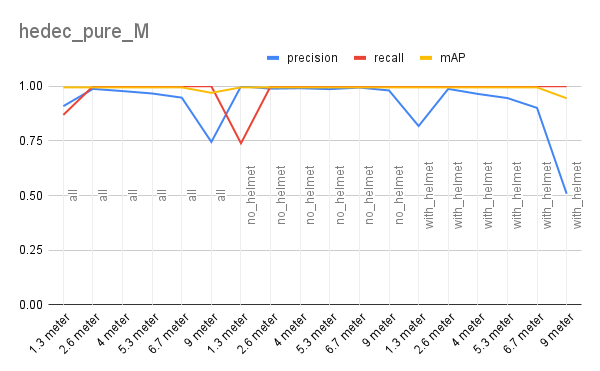
\includegraphics[width=1\textwidth]{gambar/BerdasarkanJarak/hedec_pure_M.png}
    \caption{Grafik \emph{Precision, Recall, mAP} untuk \textbf{"hedec\_pure\_M"} Pada Jarak 1.3 meter Hingga 9 meter}
    \label{fig:grafvaljarak_hedec_pure_M}  
  \end{figure}

  \begin{figure} [h!]
    \centering
    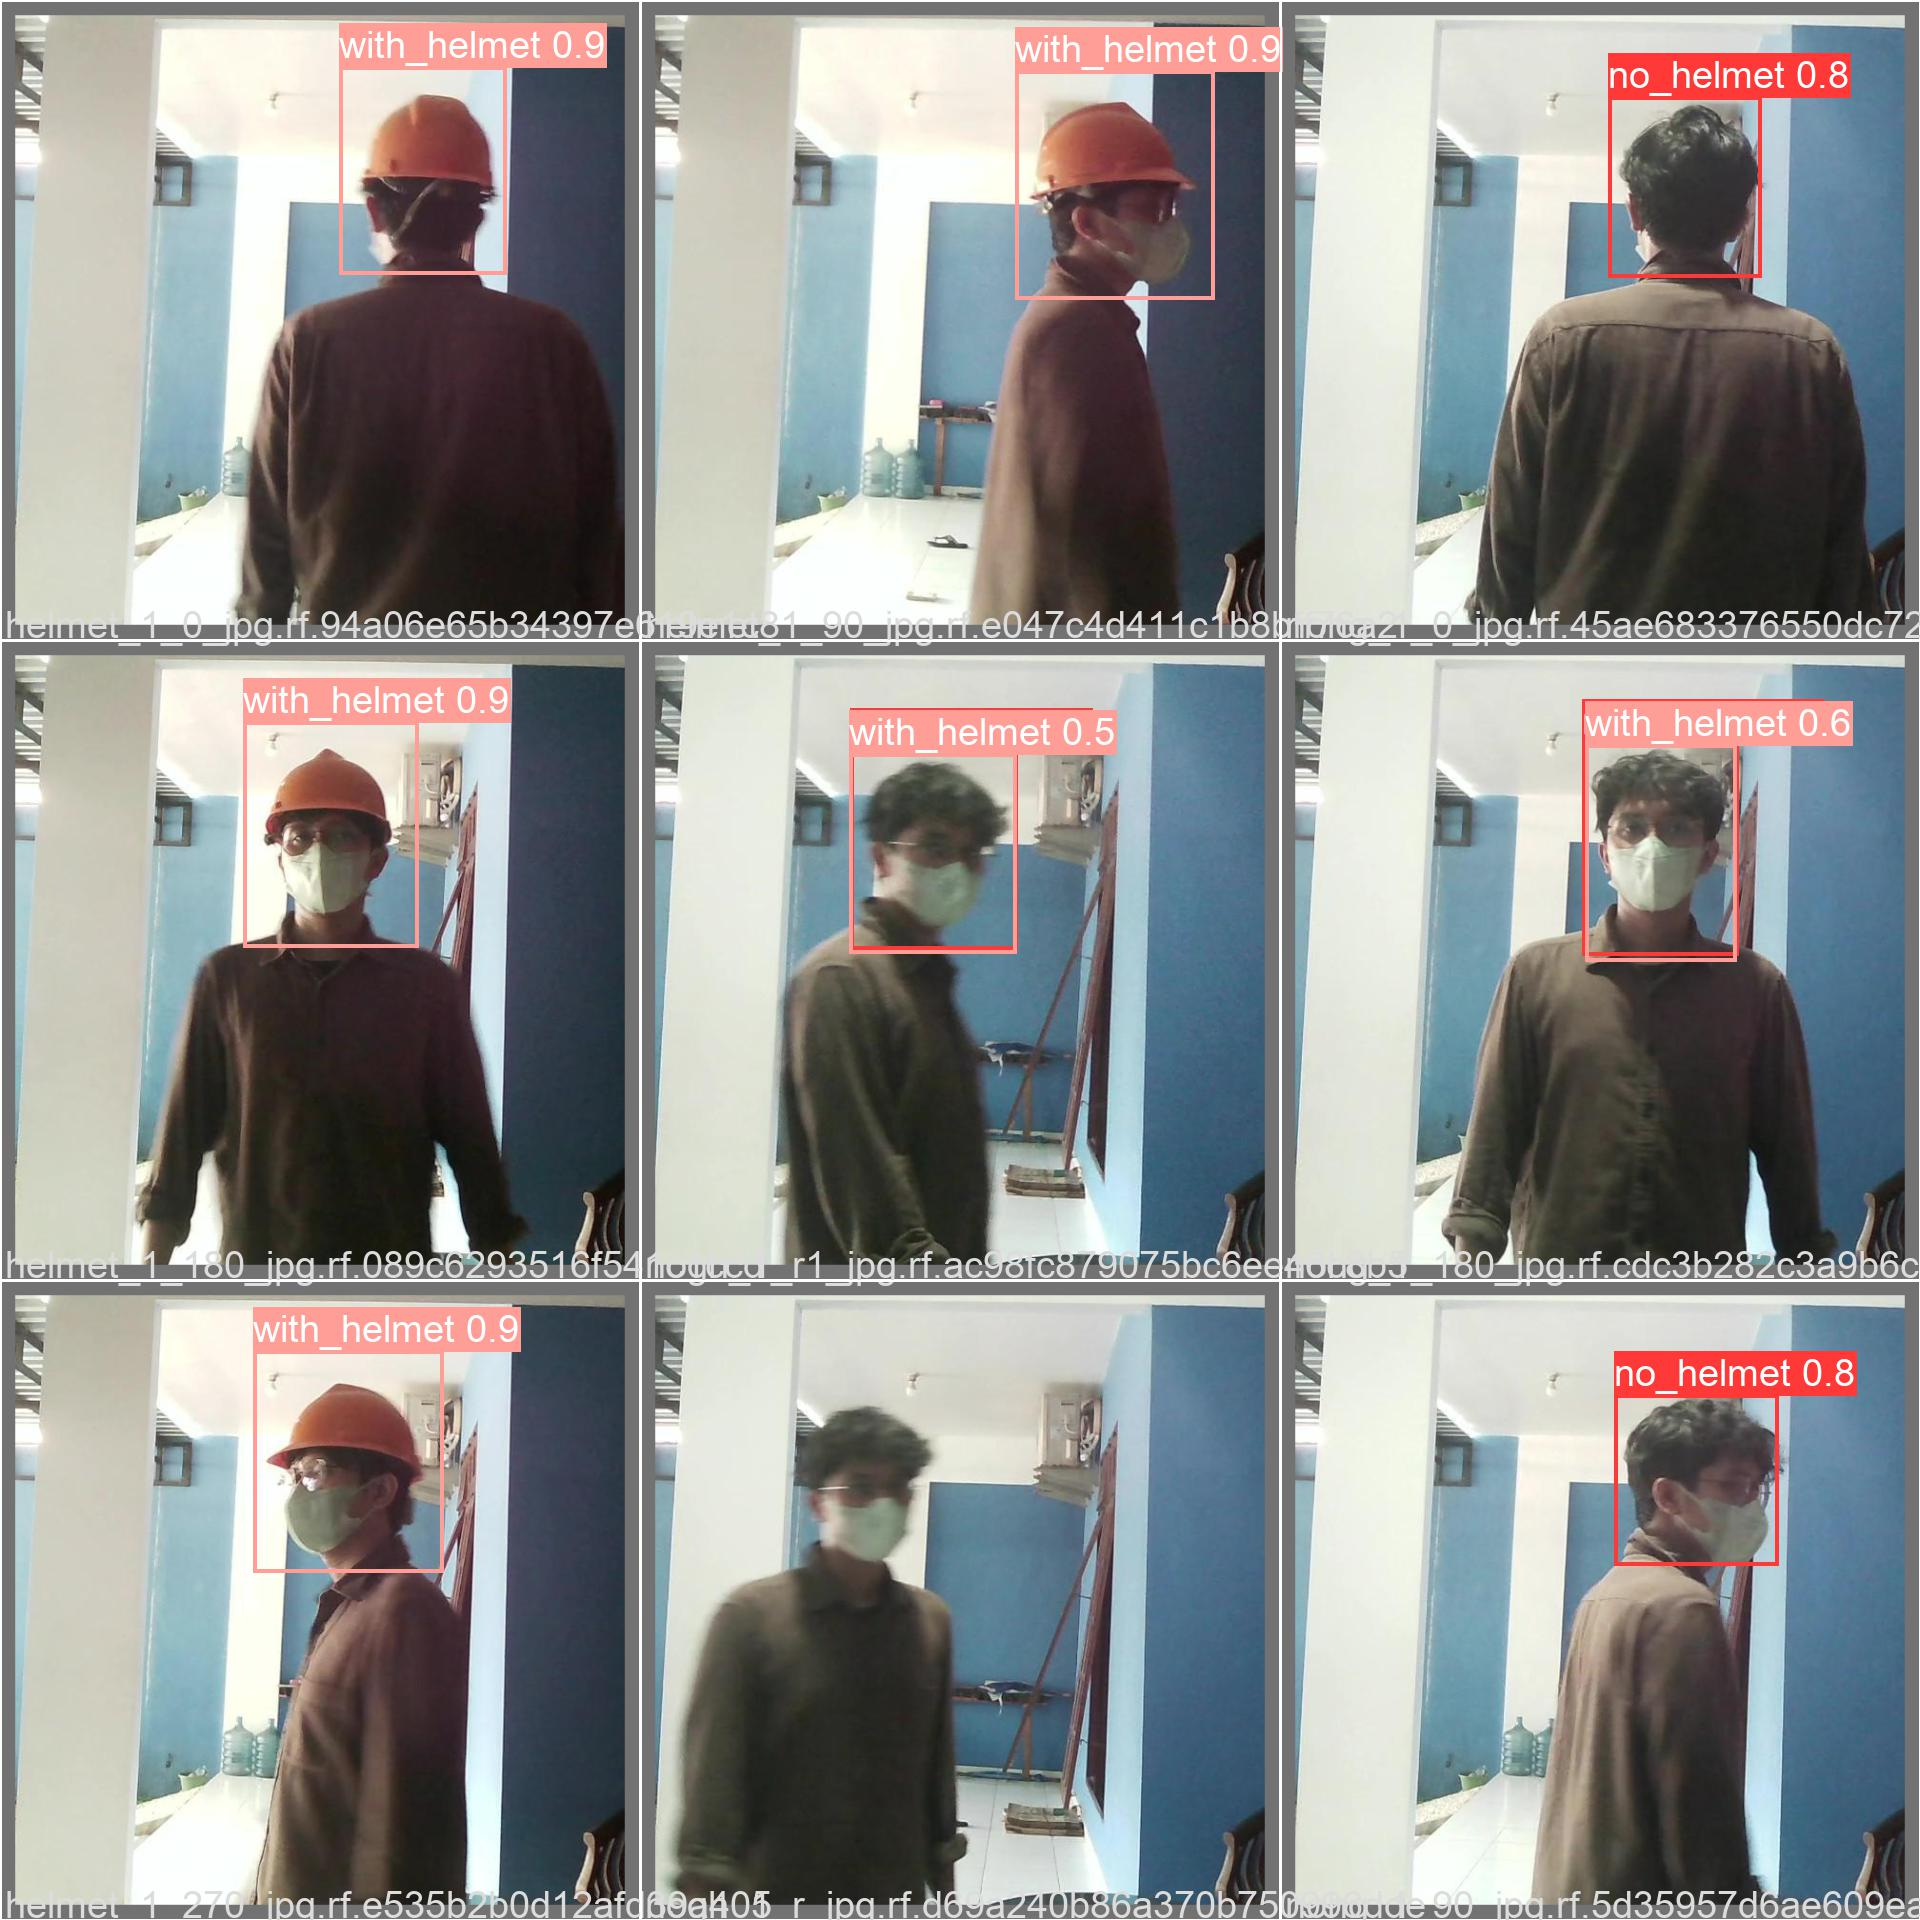
\includegraphics[width=0.3\textwidth]{gambar/BerdasarkanJarak_v2/val_hedec_pure_M/Jarak1_3/val_batch0_pred.jpg}
    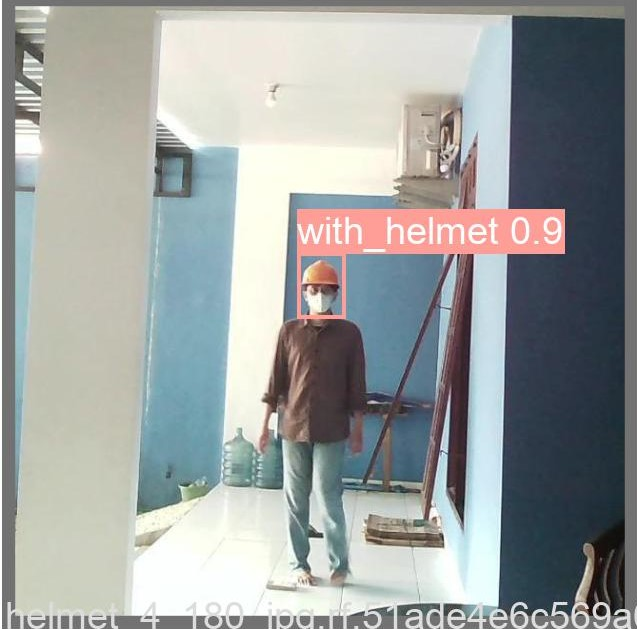
\includegraphics[width=0.3\textwidth]{gambar/BerdasarkanJarak_v2/val_hedec_pure_M/Jarak5_3/val_batch0_pred.jpg}
    \includegraphics[width=0.3\textwidth]{gambar/BerdasarkanJarak_v2/val_hedec_pure_M/Jarak9/val_batch0_pred.jpg}
    \caption{Hasil Prediksi Untuk Bobot "hedec\_pure\_M" Pada Perbedaan Jarak}
    \label{fig:valjarak_sample_hedec_pure_M}  
  \end{figure}

   \newpage
  \item \textbf{hedec\_pure\_L}
  
  \par Pada pengujian pada jarak berbeda dari 1.3 meter hingga 9 meter untuk bobot "hedec\_pure\_L" yang merupakan bobot hasil \emph{training}
  yang tidak menggunakan \emph{Pretrained Weights} dari repository YOLOv5 tetapi konfigurasinya menyerupai konfigurasi
  varian \emph{Pretrained Weights} varian YOLOv5l memeiliki beberapa poin yang dapat ditarik. 
  Seperti yang bisa dilihat pada Gambar~\ref{fig:grafvaljarak_hedec_pure_L},
  pada jarak 1.3 meter memiliki nilai yang sedikit rendah untuk \emph{precision, recall} (0.842 dan 0.871) jika dibandingkan dengan jarak 2.6 meter hingga 6.7 meter. 
  Lalu \emph{precision} untuk kelas "with\_helmet" mengalami penurunan drastis pada jarak 9 meter yaitu 0.598.
  Tidak seperti untuk bobot sebandingnya yaitu "hedec\_pretain\_L" yang memiliki hasil validasi yang semua berada di atas 0.9, bobot "hedec\_pure\_L" memiliki penurunan
  pada jarak 9 meter.
  Tabel untuk hasil validasi dari "hedec\_pure\_L" bisa dilihat
  pada Tabel~\ref{tb:hasiljarak_hedec_pure_L}.
  
  \begin{longtable}{|l|l|l|l|l|} 
    \caption{Hasil Validasi Perbedaan Jarak Pada \textbf{"hedec\_pure\_L"}}
    \label{tb:hasiljarak_hedec_pure_L}\\
    \hline
    Jarak     & class        & precision & recall & mAP    \\ 
    \hline
    1.3 meter & all          & 0.842     & 0.871  & 0.978  \\
    2.6 meter & all          & 0.98      & 1      & 0.995  \\
    4 meter   & all          & 0.977     & 1      & 0.995  \\
    5.3 meter & all          & 0.874     & 0.99   & 0.995  \\
    6.7 meter & all          & 0.972     & 1      & 0.995  \\
    9 meter   & all          & 0.794     & 0.849  & 0.995  \\
    1.3 meter & no\_helmet   & 1         & 0.741  & 0.962  \\
    2.6 meter & no\_helmet   & 0.988     & 1      & 0.995  \\
    4 meter   & no\_helmet   & 0.99      & 1      & 0.995  \\
    5.3 meter & no\_helmet   & 1         & 0.98   & 0.995  \\
    6.7 meter & no\_helmet   & 0.987     & 1      & 0.995  \\
    9 meter   & no\_helmet   & 1         & 0.698  & 0.995  \\
    1.3 meter & with\_helmet & 0.683     & 1      & 0.995  \\
    2.6 meter & with\_helmet & 0.971     & 1      & 0.995  \\
    4 meter   & with\_helmet & 0.964     & 1      & 0.995  \\
    5.3 meter & with\_helmet & 0.749     & 1      & 0.995  \\
    6.7 meter & with\_helmet & 0.956     & 1      & 0.995  \\
    9 meter   & with\_helmet & 0.589     & 1      & 0.995  \\
    \hline
  \end{longtable}

  \newpage
  \begin{figure} [h!]
    \centering
    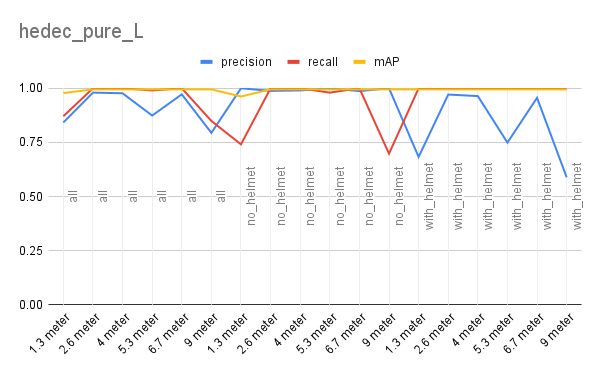
\includegraphics[width=1\textwidth]{gambar/BerdasarkanJarak/hedec_pure_L.png}
    \caption{Grafik \emph{Precision, Recall, mAP} untuk \textbf{"hedec\_pure\_L"} Pada Jarak 1.3 meter Hingga 9 meter}
    \label{fig:grafvaljarak_hedec_pure_L}  
  \end{figure}

  \begin{figure} [h!]
    \centering
    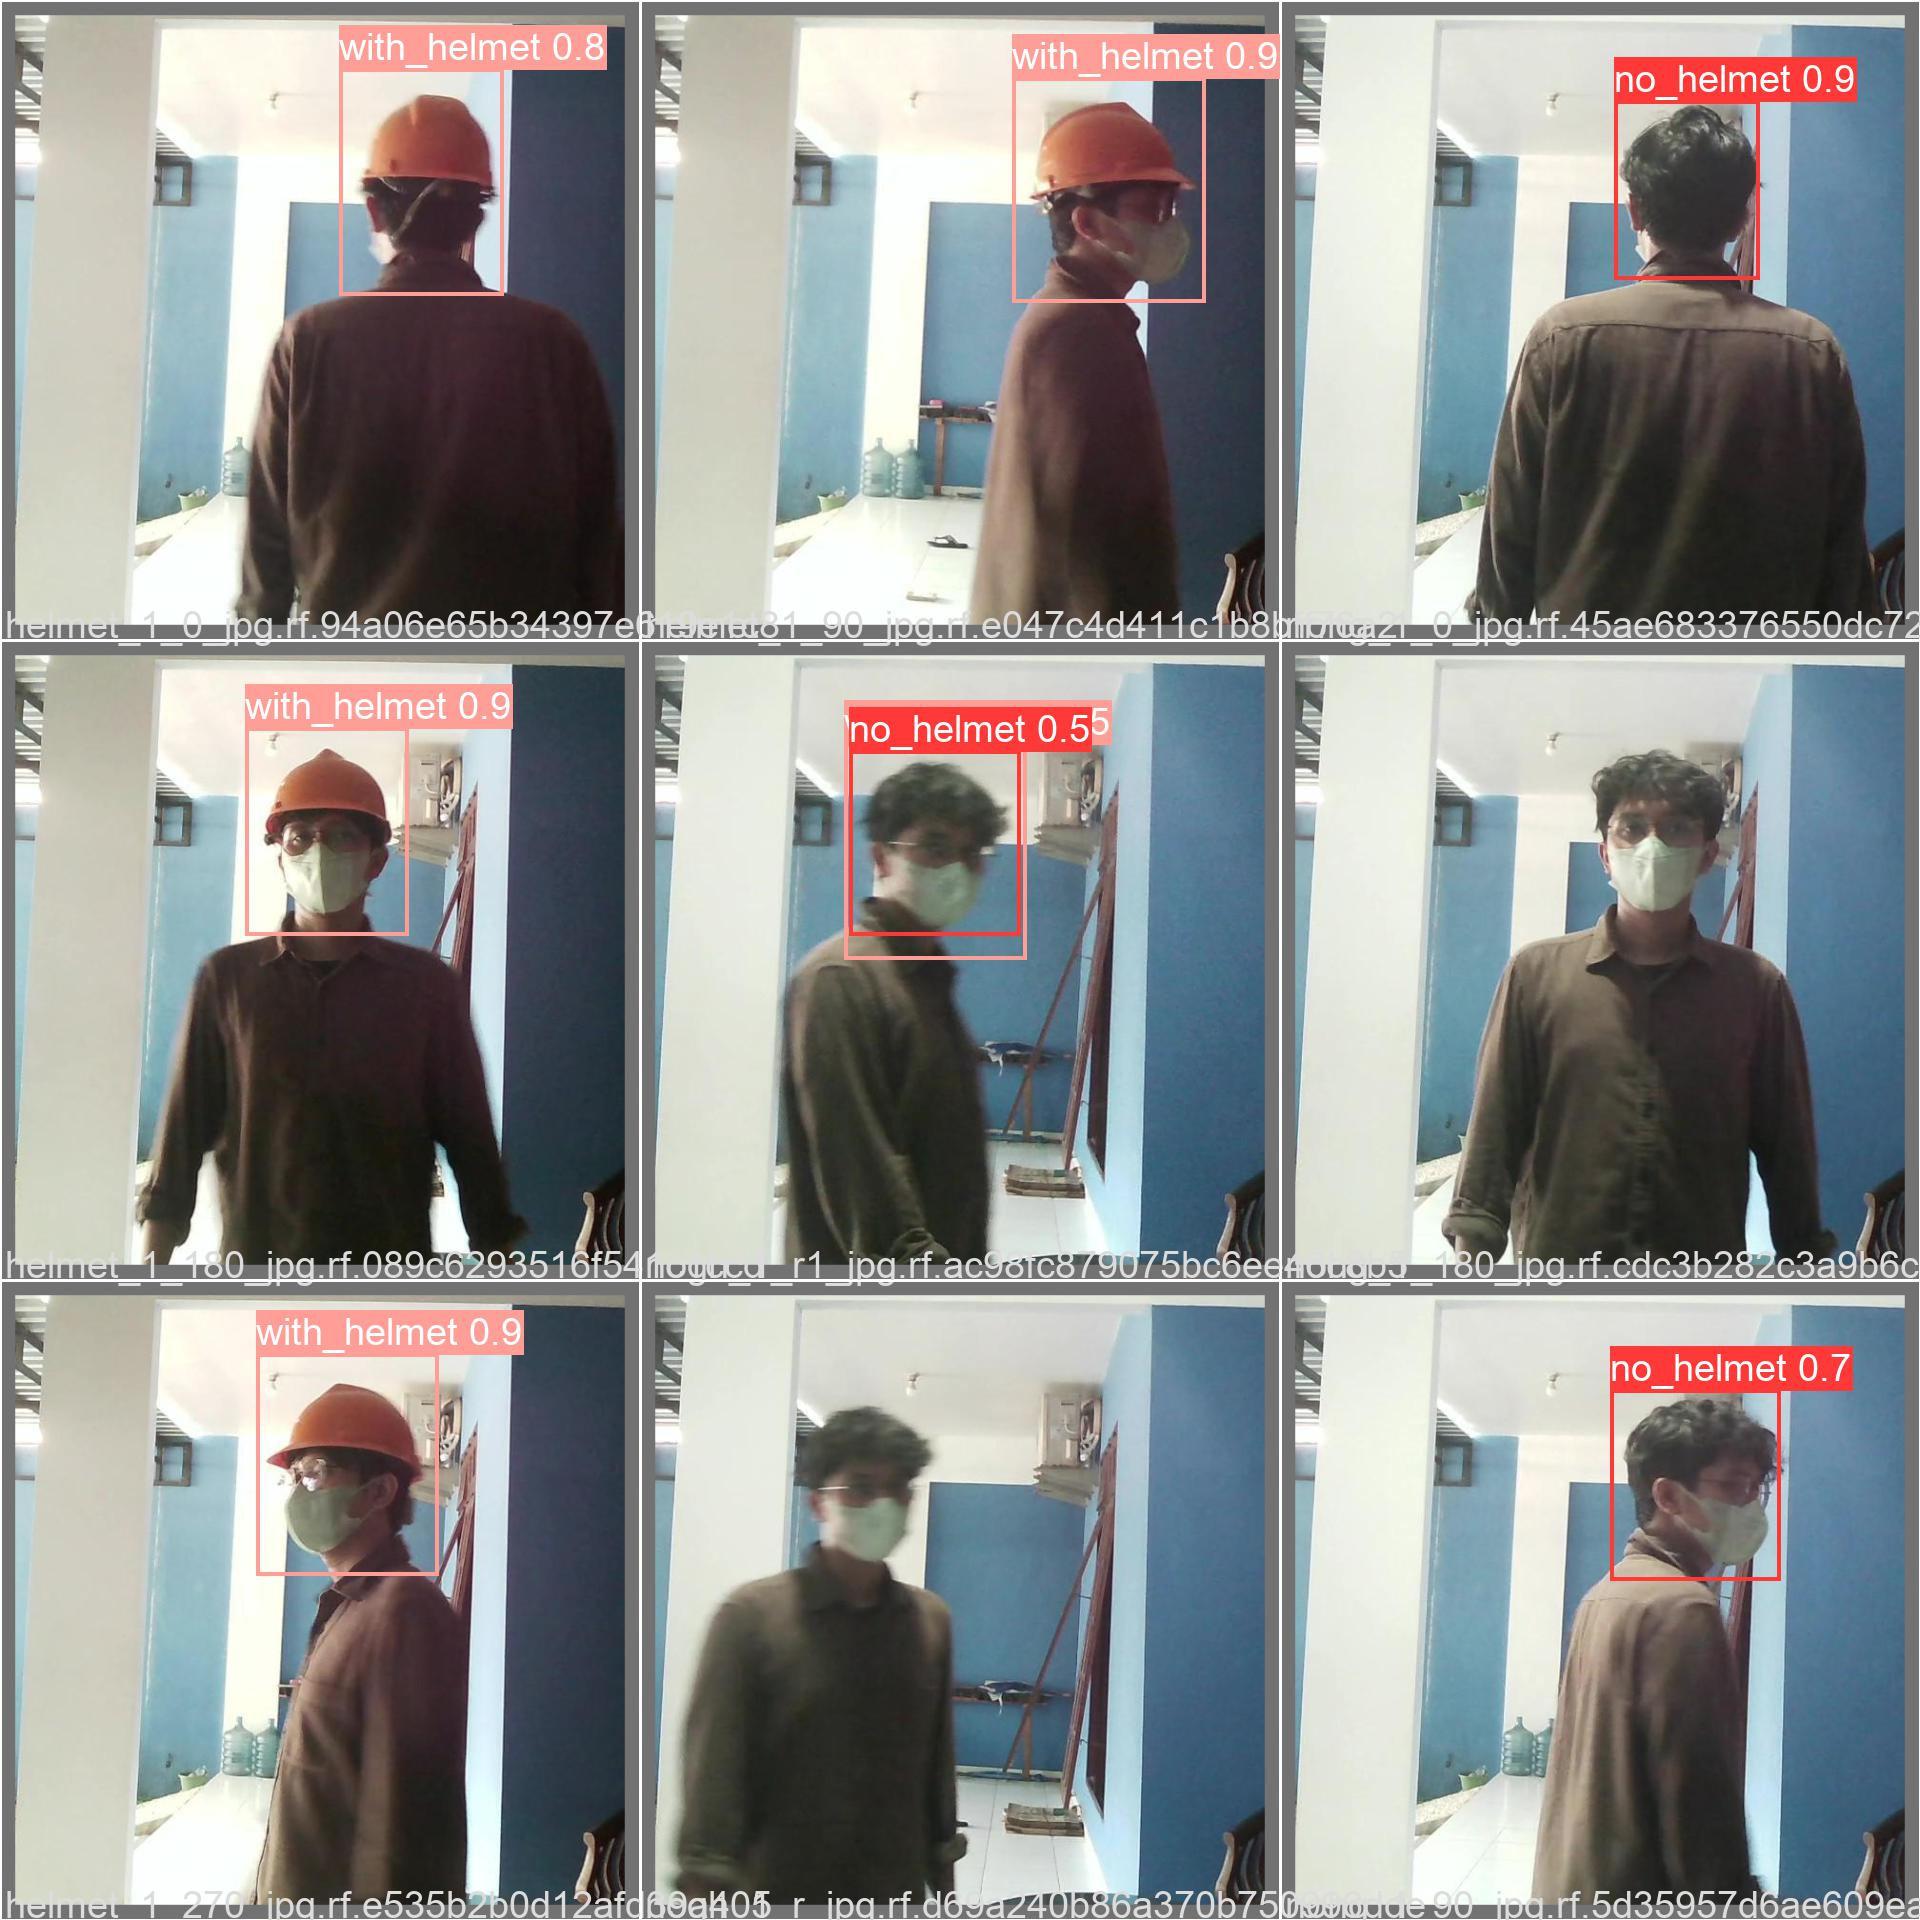
\includegraphics[width=0.3\textwidth]{gambar/BerdasarkanJarak_v2/val_hedec_pure_L/Jarak1_3/val_batch0_pred.jpg}
    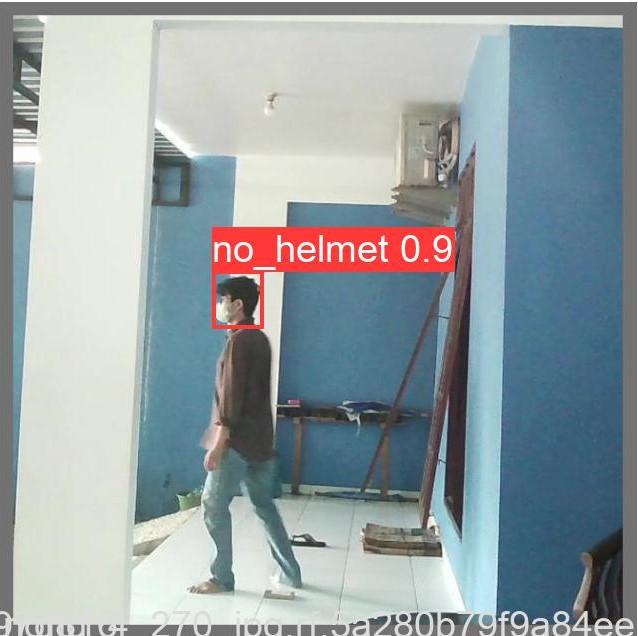
\includegraphics[width=0.3\textwidth]{gambar/BerdasarkanJarak_v2/val_hedec_pure_L/Jarak5_3/val_batch0_pred.jpg}
    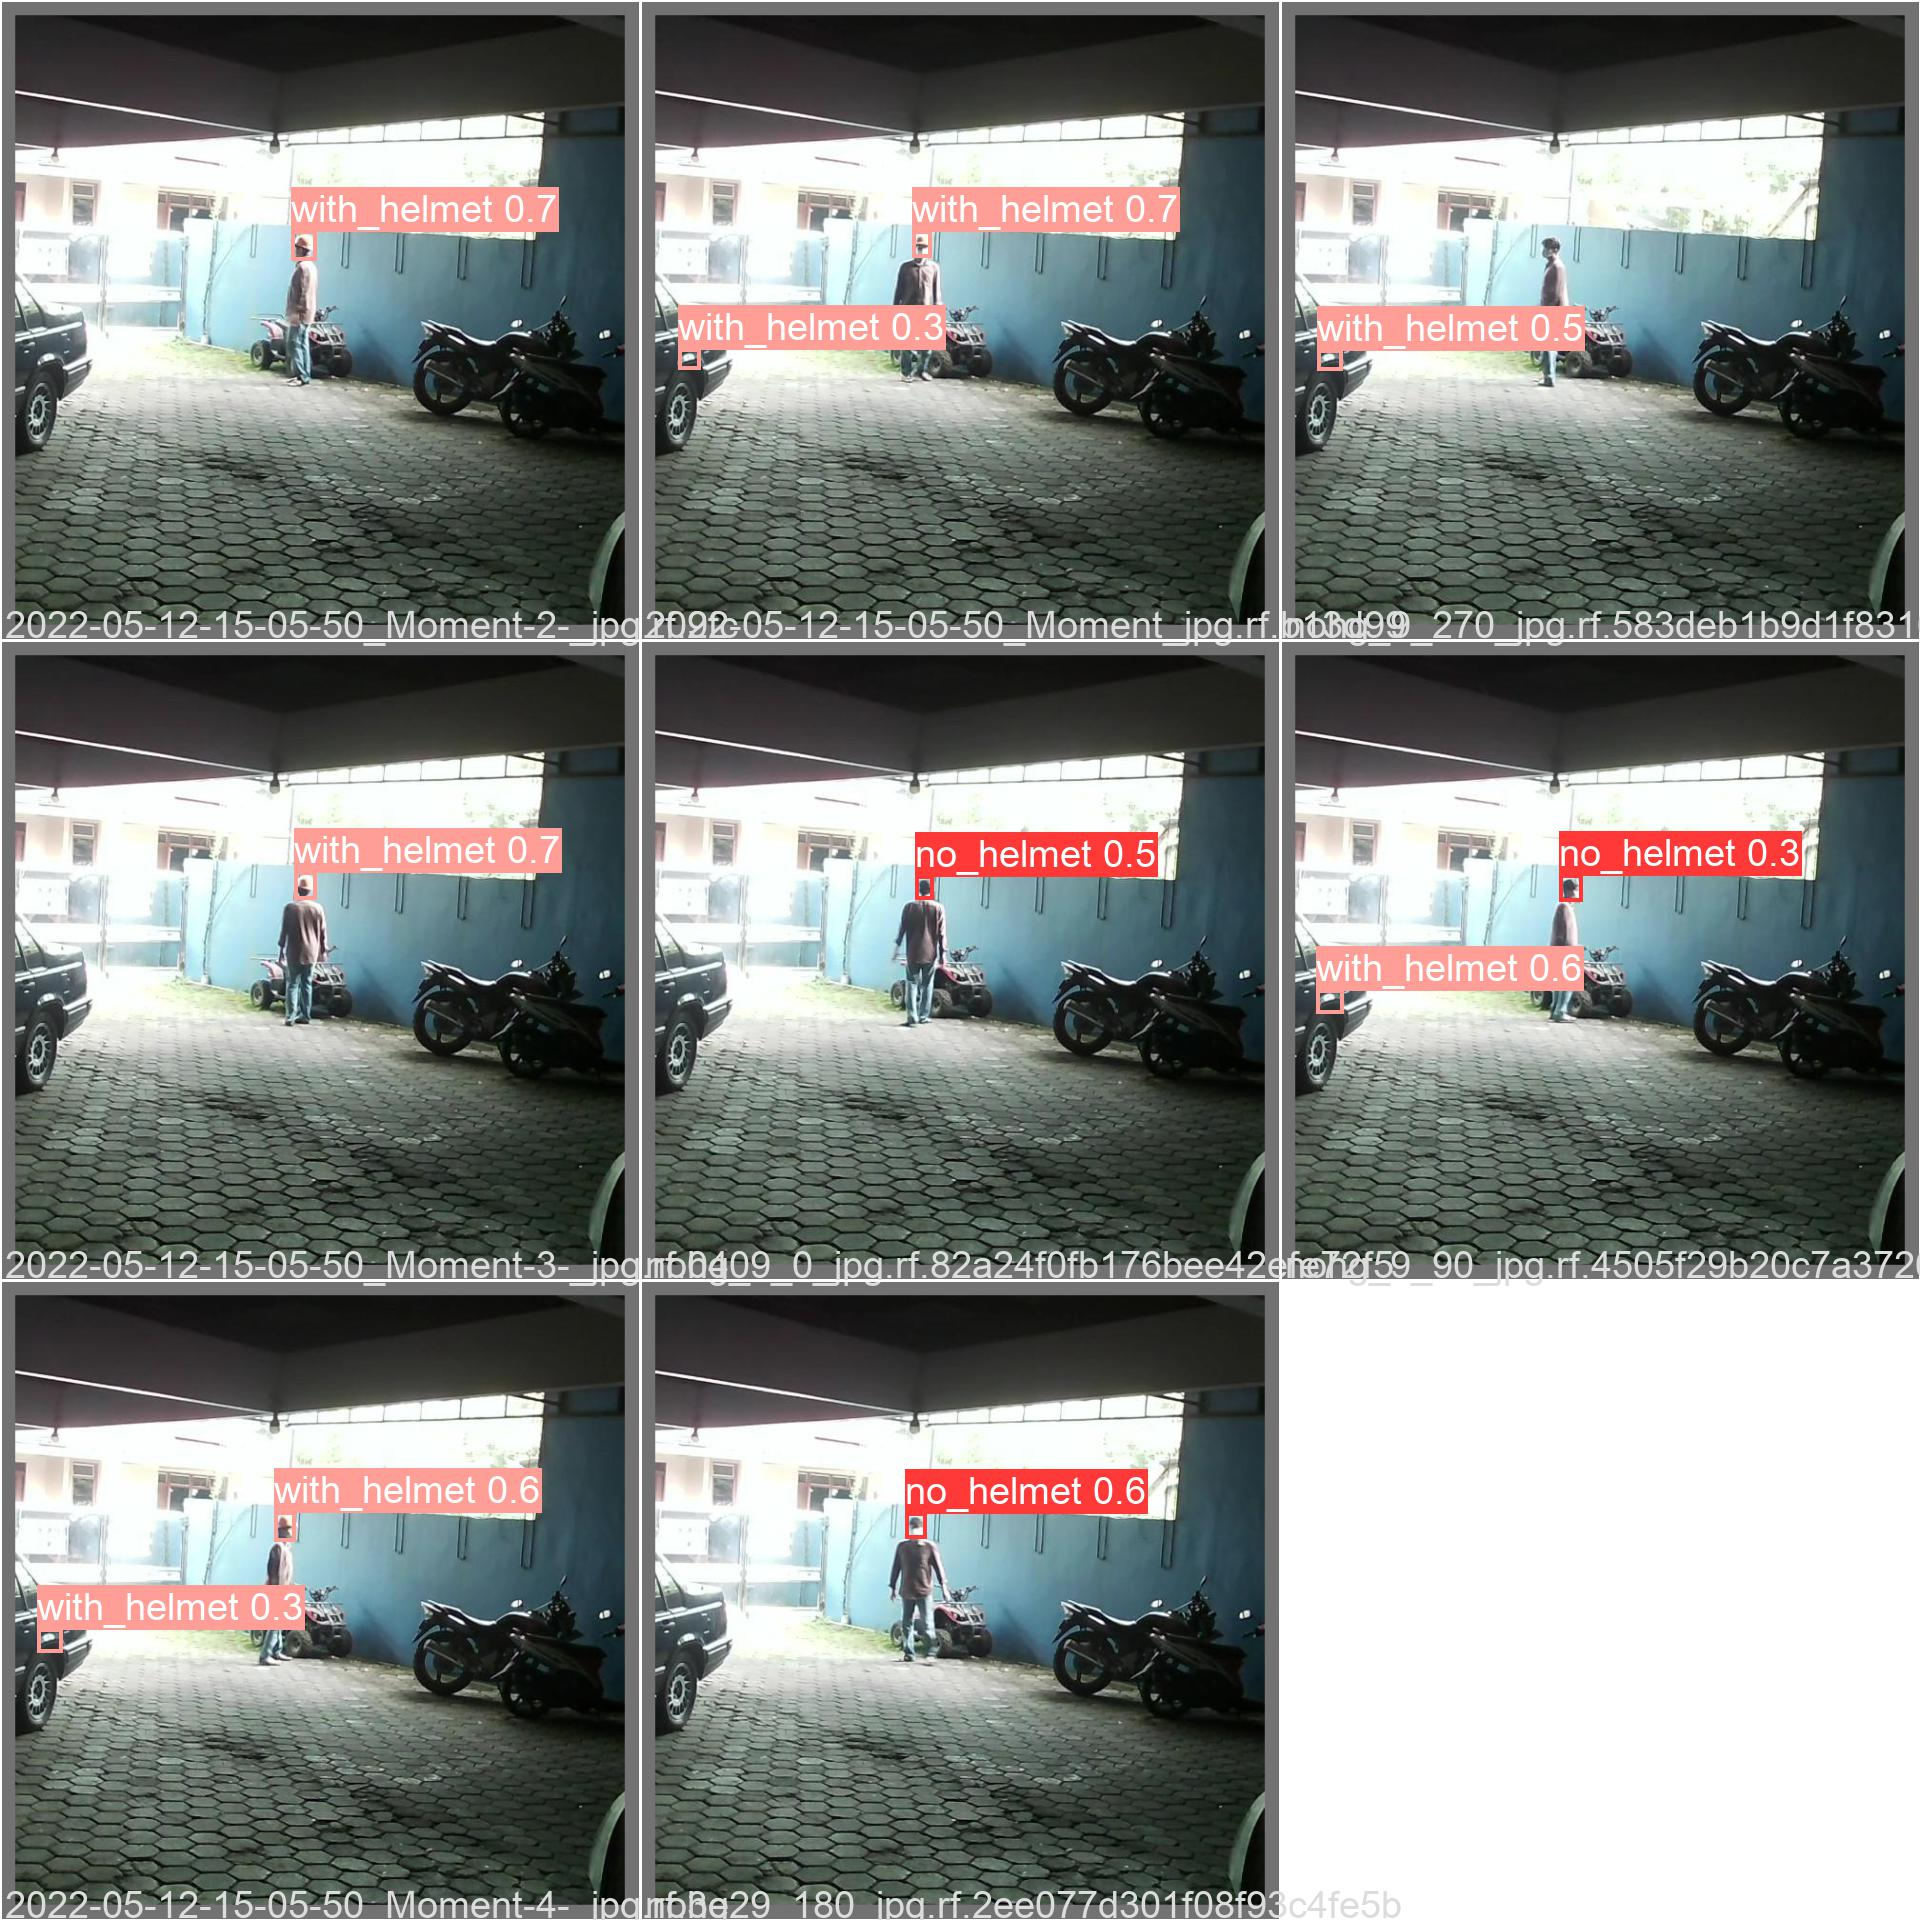
\includegraphics[width=0.3\textwidth]{gambar/BerdasarkanJarak_v2/val_hedec_pure_L/Jarak9/val_batch0_pred.jpg}
    \caption{Hasil Prediksi Untuk Bobot "hedec\_pure\_L" Pada Perbedaan Jarak}
    \label{fig:valjarak_sample_hedec_pure_L}  
  \end{figure}



\end{enumerate}



% \newpage
\newpage
\section{Pengujian Pada Tingkat Kecerahan Rendah}
\label{sec:pengujianberdasarkantingkatkeceharan}

\par Bagian ini memaparkan performa model melakukan
deteksi pada input gambar dengan tingkat kecerahan rendah. Data validasi berisi
35 gambar dengan jumlah label \emph{no\textunderscore helmet} 20 dan label \emph{with\textunderscore helmet} 57.
Validasi dilakukan pada bobot hasil training yang menggunakan \textit{pretrained weight} dan yang tanpa menggunakan \textit{pretrained weight}. 

\subsection{Pengujian Pada Tingkat Kecerahan Rendah dengan \emph{Pretrained Weight}}
\label{subsec:lowlight_pretrained}

\par Berikut merupakan pemaparan hasil validasi pada data validasi menggunakan \emph{weight} yang di-\emph{train} menggunakan
\emph{pretrained weights} yang disedikan repo YOLOv5 yang selanjutnya disebut sebagai "hedec\textunderscore pretain". 
Seperti yang dijelaskan pada Subbab~\ref{subsec:ujiperforma_coco}. 


\begin{enumerate}
  \item \textbf{hedec\textunderscore pretrain\textunderscore N}
  
  \par Dilakukan pengujian kecerahan rendah dengan menggunakan bobot yang di-\emph{train} menggunakan bobot
  pretrain COCO untuk varian \emph{nano} yang merupakan varian paling kecil dari semua bobot yang disediakan 
  dari repo. Didapatkan rata - rata presisi untuk semua kelas 0.767 dan \emph{recall} untuk semua kelas 0.373.
  \par Didapati untuk kelas \emph{no\textunderscore helmet} mendapatkan nilai \emph{precision} 1 dan \emph{recall}
  0. Hal ini dikarenakan objek kepala tanpa menggunakan helm tidak ada yang terdektsi dan atau terdeteksi
  sebagai kelas \emph{with\textunderscore helmet}. 
  
  \begin{longtable}{|c|c|c|c|}
    \caption{Hasil Validasi Pada Tingkat Kecerahan Rendah dengan hedec\textunderscore pretrain\textunderscore N   }
    \label{tb:validasitingkatacerahrendah_yolo5n}\\
    \hline
    % \rowcolor[HTML]{C0C0C0}
    \textbf{\emph{Class} }                     & \textbf{\emph{Precision}}  & \textbf{\emph{Recall}} & \textbf{\emph{mAP@.5}}\\
    \hline
    all                                                 & 0.767          & 0.373        & 0.415         \\
    no\textunderscore helmet                            & 1              & 0            & 0.143          \\
    with\textunderscore helmet                          & 0.534          & 0.745        & 0.687         \\
    \hline
  \end{longtable}
  
  \begin{figure}[h]
    \centering
    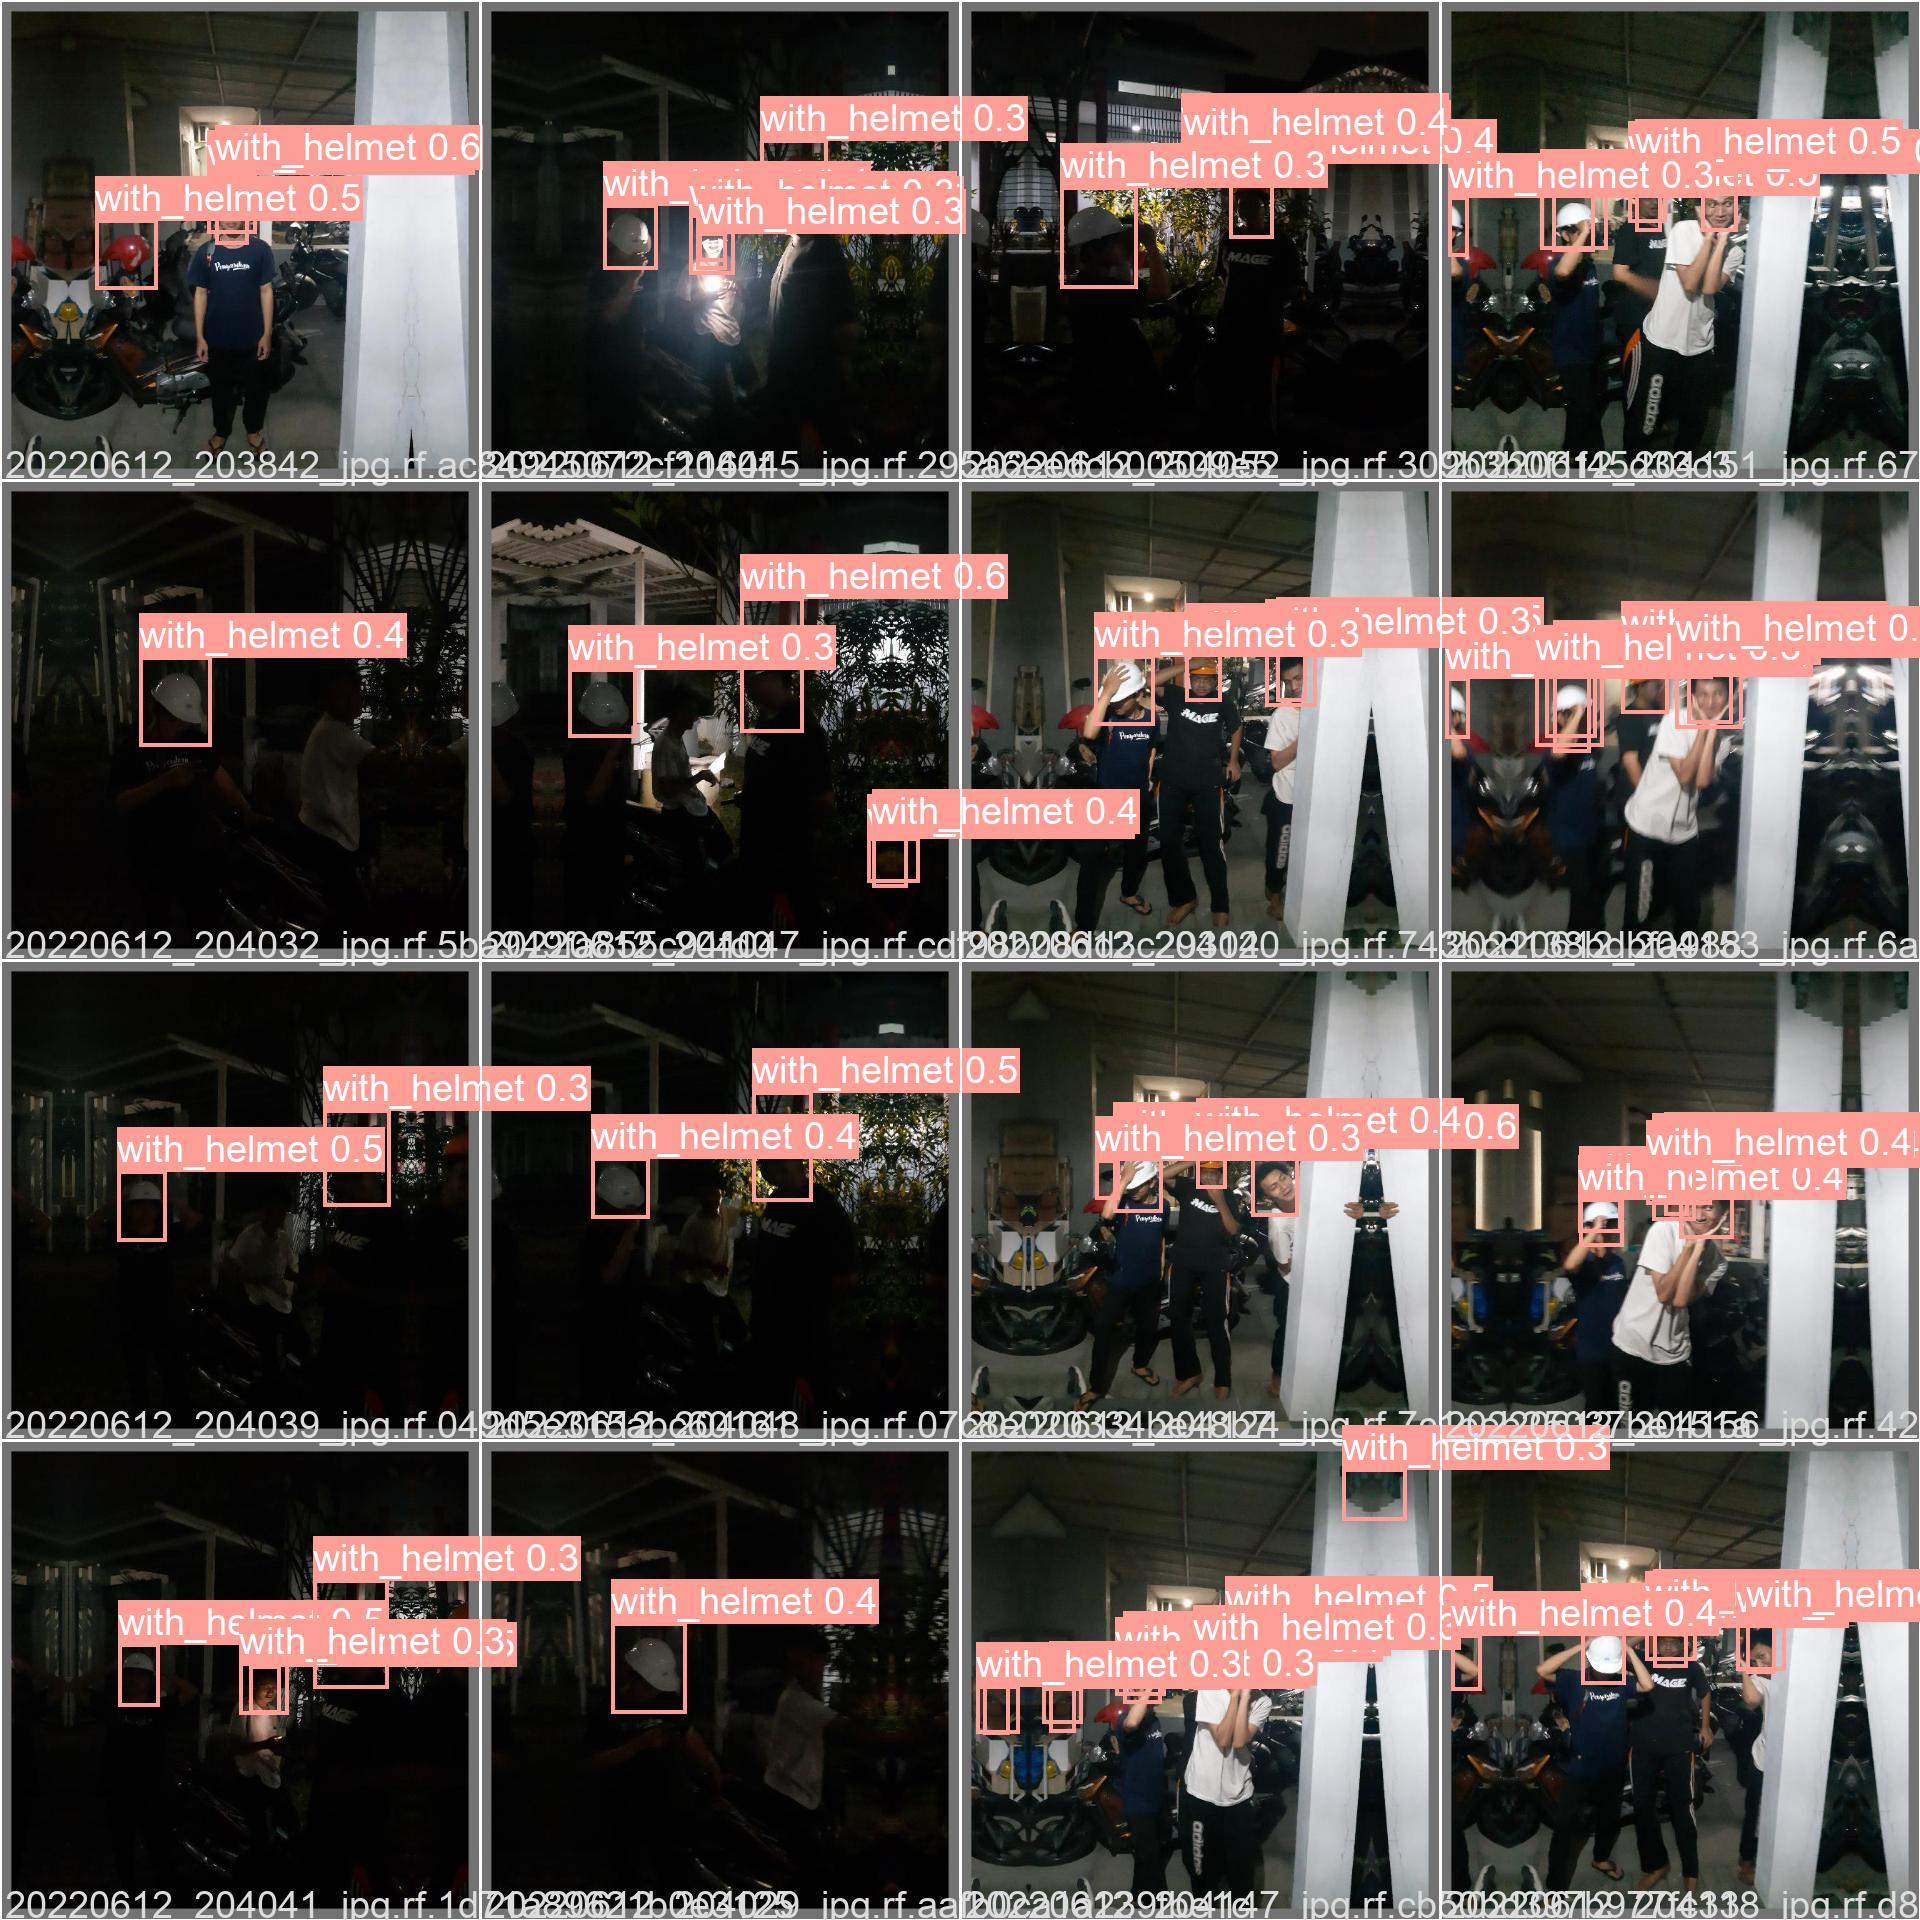
\includegraphics[scale=0.2]{gambar/train_v2_val/low_ligjt/yolonano/val_batch0_pred.jpg}
    % \includegraphics[scale=0.1]{gambar/train_v2_val/low_ligjt/yolonano/val_batch0_labels.jpg}
    \caption{Hasil Prediksi Pada Keadaan Rendah dengan hedec\textunderscore pretrain\textunderscore N    }
    % \label{fig:labelbaru}  
  \end{figure}

  \FloatBarrier
   
  \item \textbf{hedec\textunderscore pretrain\textunderscore S}
  
  \par Dilakukan pengujian kecerahan rendah dengan menggunakan bobot yang di-\emph{train} menggunakan bobot
  pretrain COCO untuk varian \emph{small}. Didapatkan rata - rata presisi untuk semua kelas 0.775 dan \emph{recall} untuk semua
  kelas 0.799. Terdapat beberapa \emph{False Positive} dalam prediksi yaitu helm motor yang diletakkan diatas
  motor diprediksi sebagai \emph{with\textunderscore helmet} begitu juga.
  
  \begin{longtable}{|c|c|c|c|}
    \caption{Hasil Validasi Pada Tingkat Kecerahan Rendah dengan hedec\textunderscore pretrain\textunderscore S}
    \label{tb:validasitingkatacerahrendah_yolov5s}\\
    \hline
    % \rowcolor[HTML]{C0C0C0}
    \textbf{\emph{Class} }                     & \textbf{\emph{Precision}}  & \textbf{\emph{Recall}} & \textbf{\emph{mAP@.5}}\\
    \hline
    all                                                 & 0.775          & 0.799        & 0.823         \\
    no\textunderscore helmet                            & 0.862           & 0.65        & 0.713          \\
    with\textunderscore helmet                          & 0.689           & 0.947        & 0.933         \\
    \hline
  \end{longtable}

  \newpage
  \begin{figure} [h!]
    \centering
    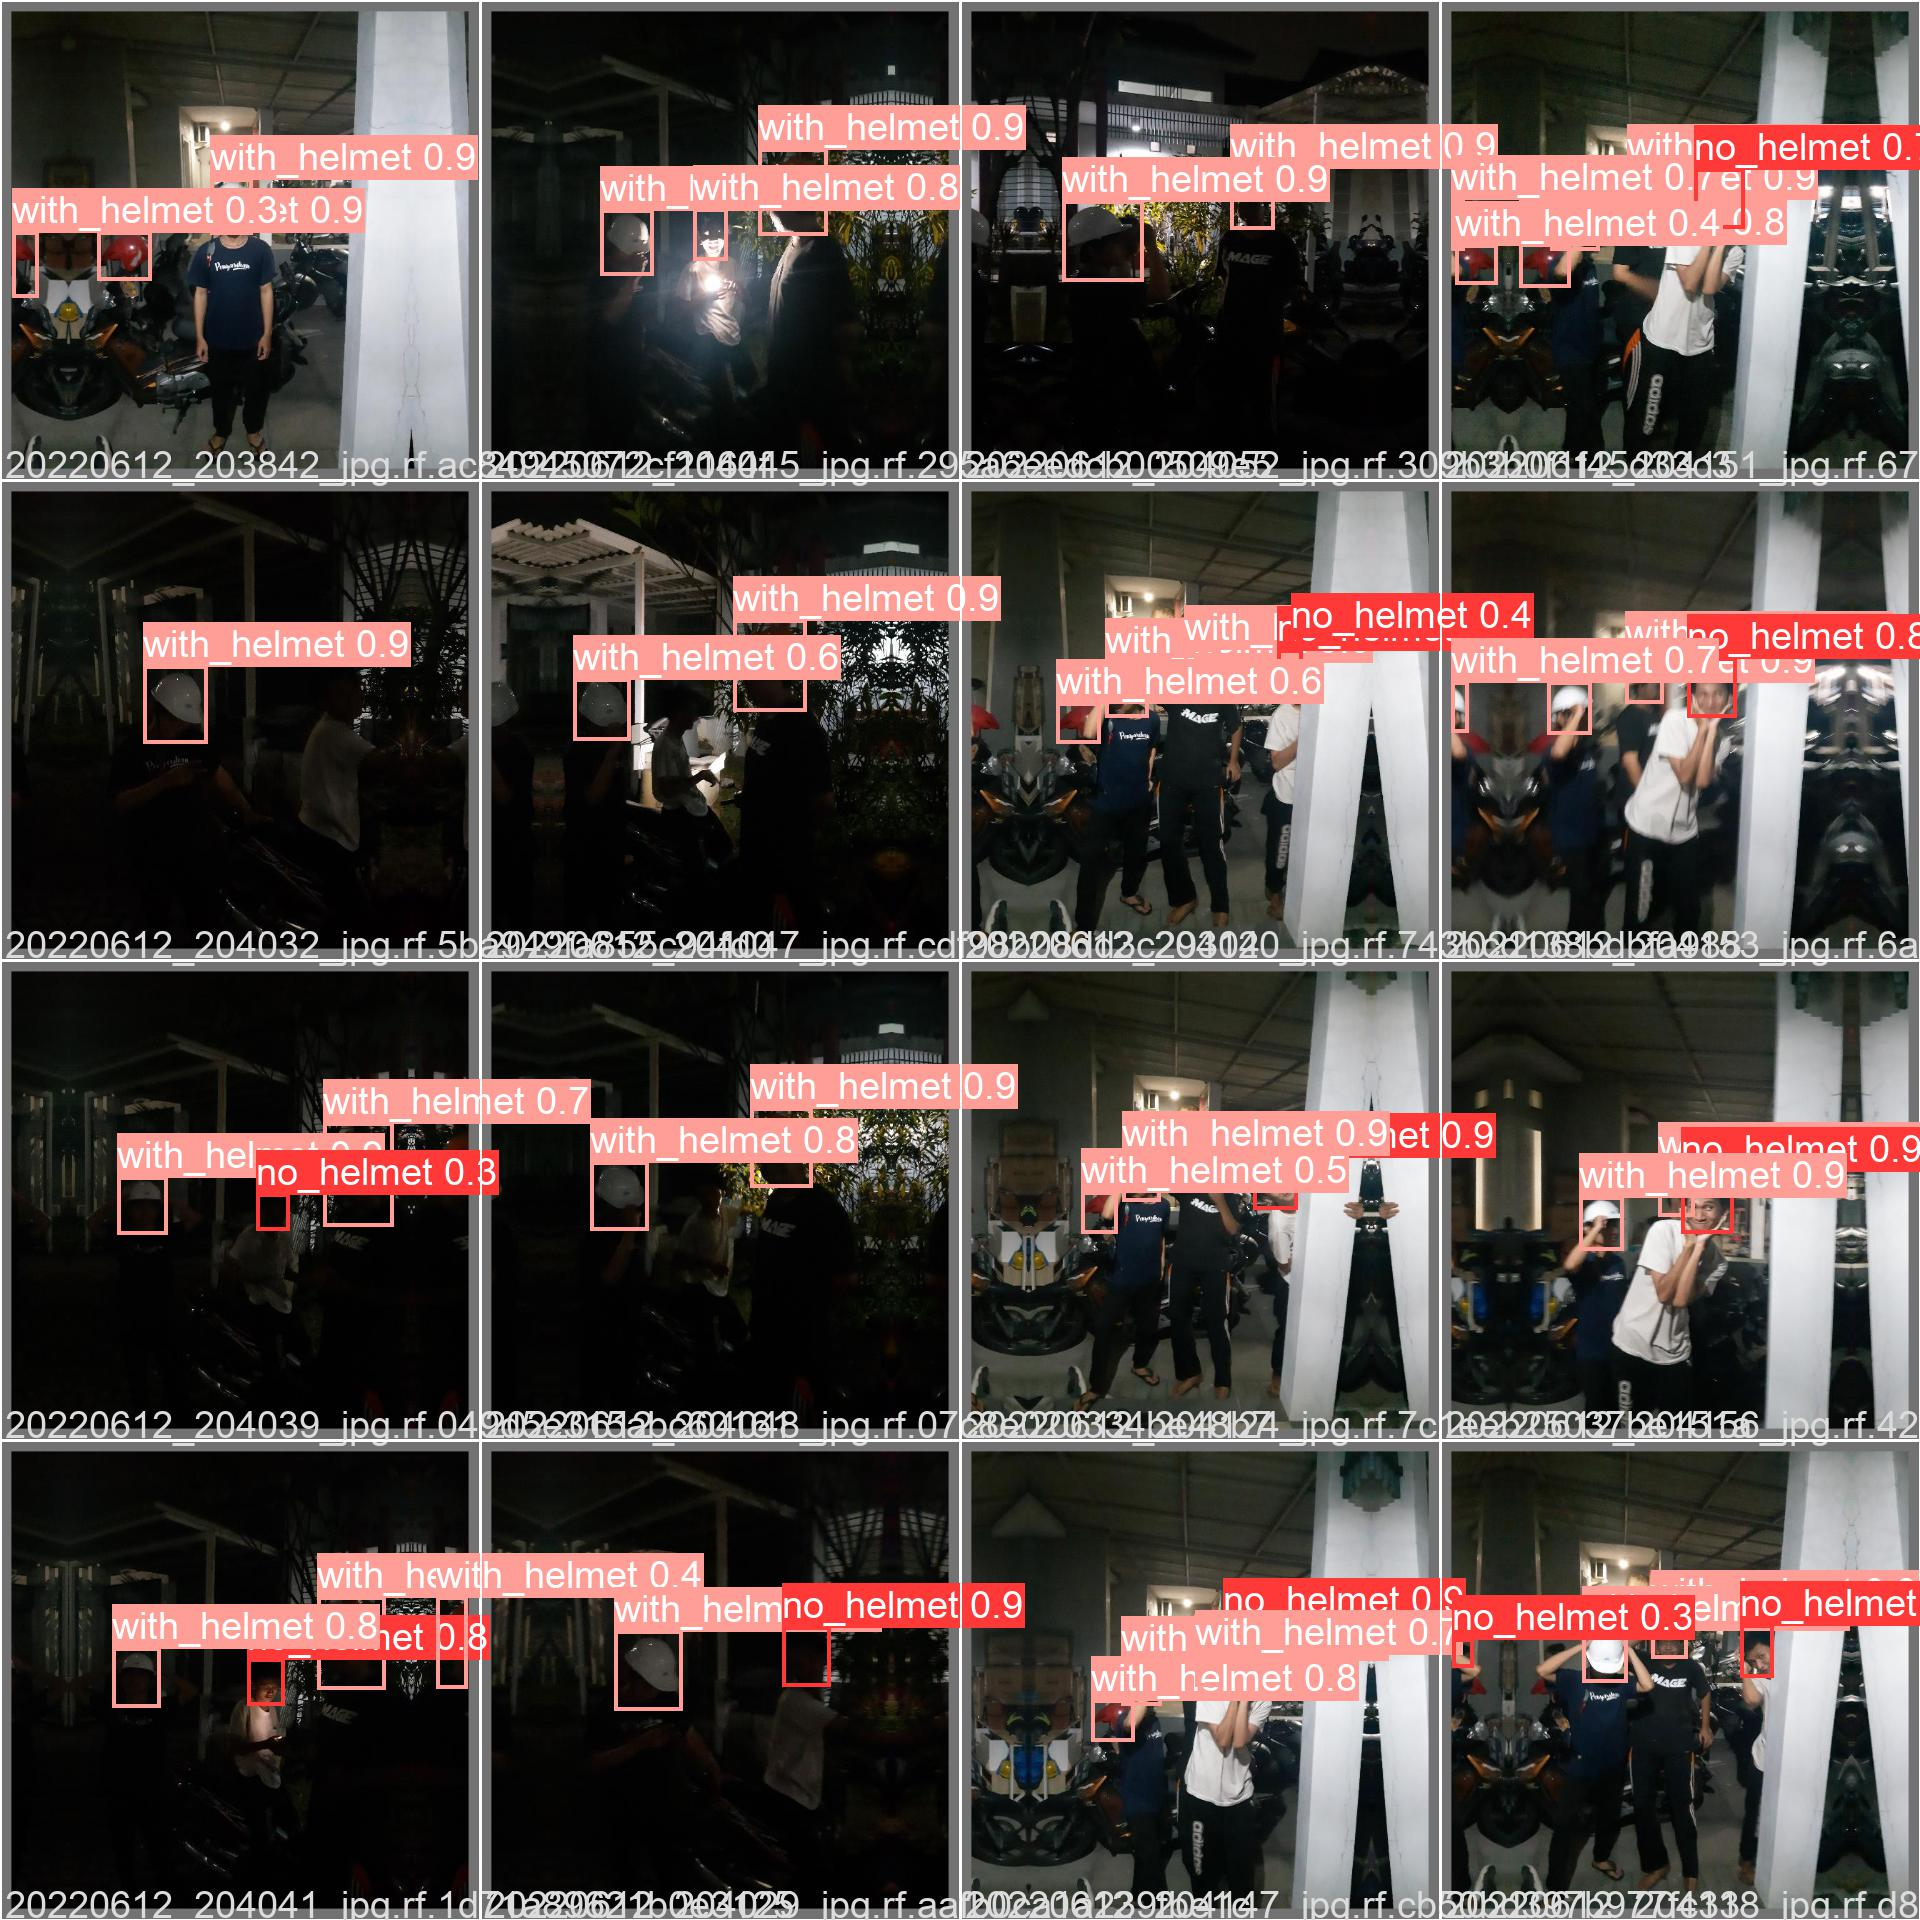
\includegraphics[scale=0.2]{gambar/train_v2_val/low_ligjt/yolosmall/low_light_val_batch0_pred.jpg}
    % 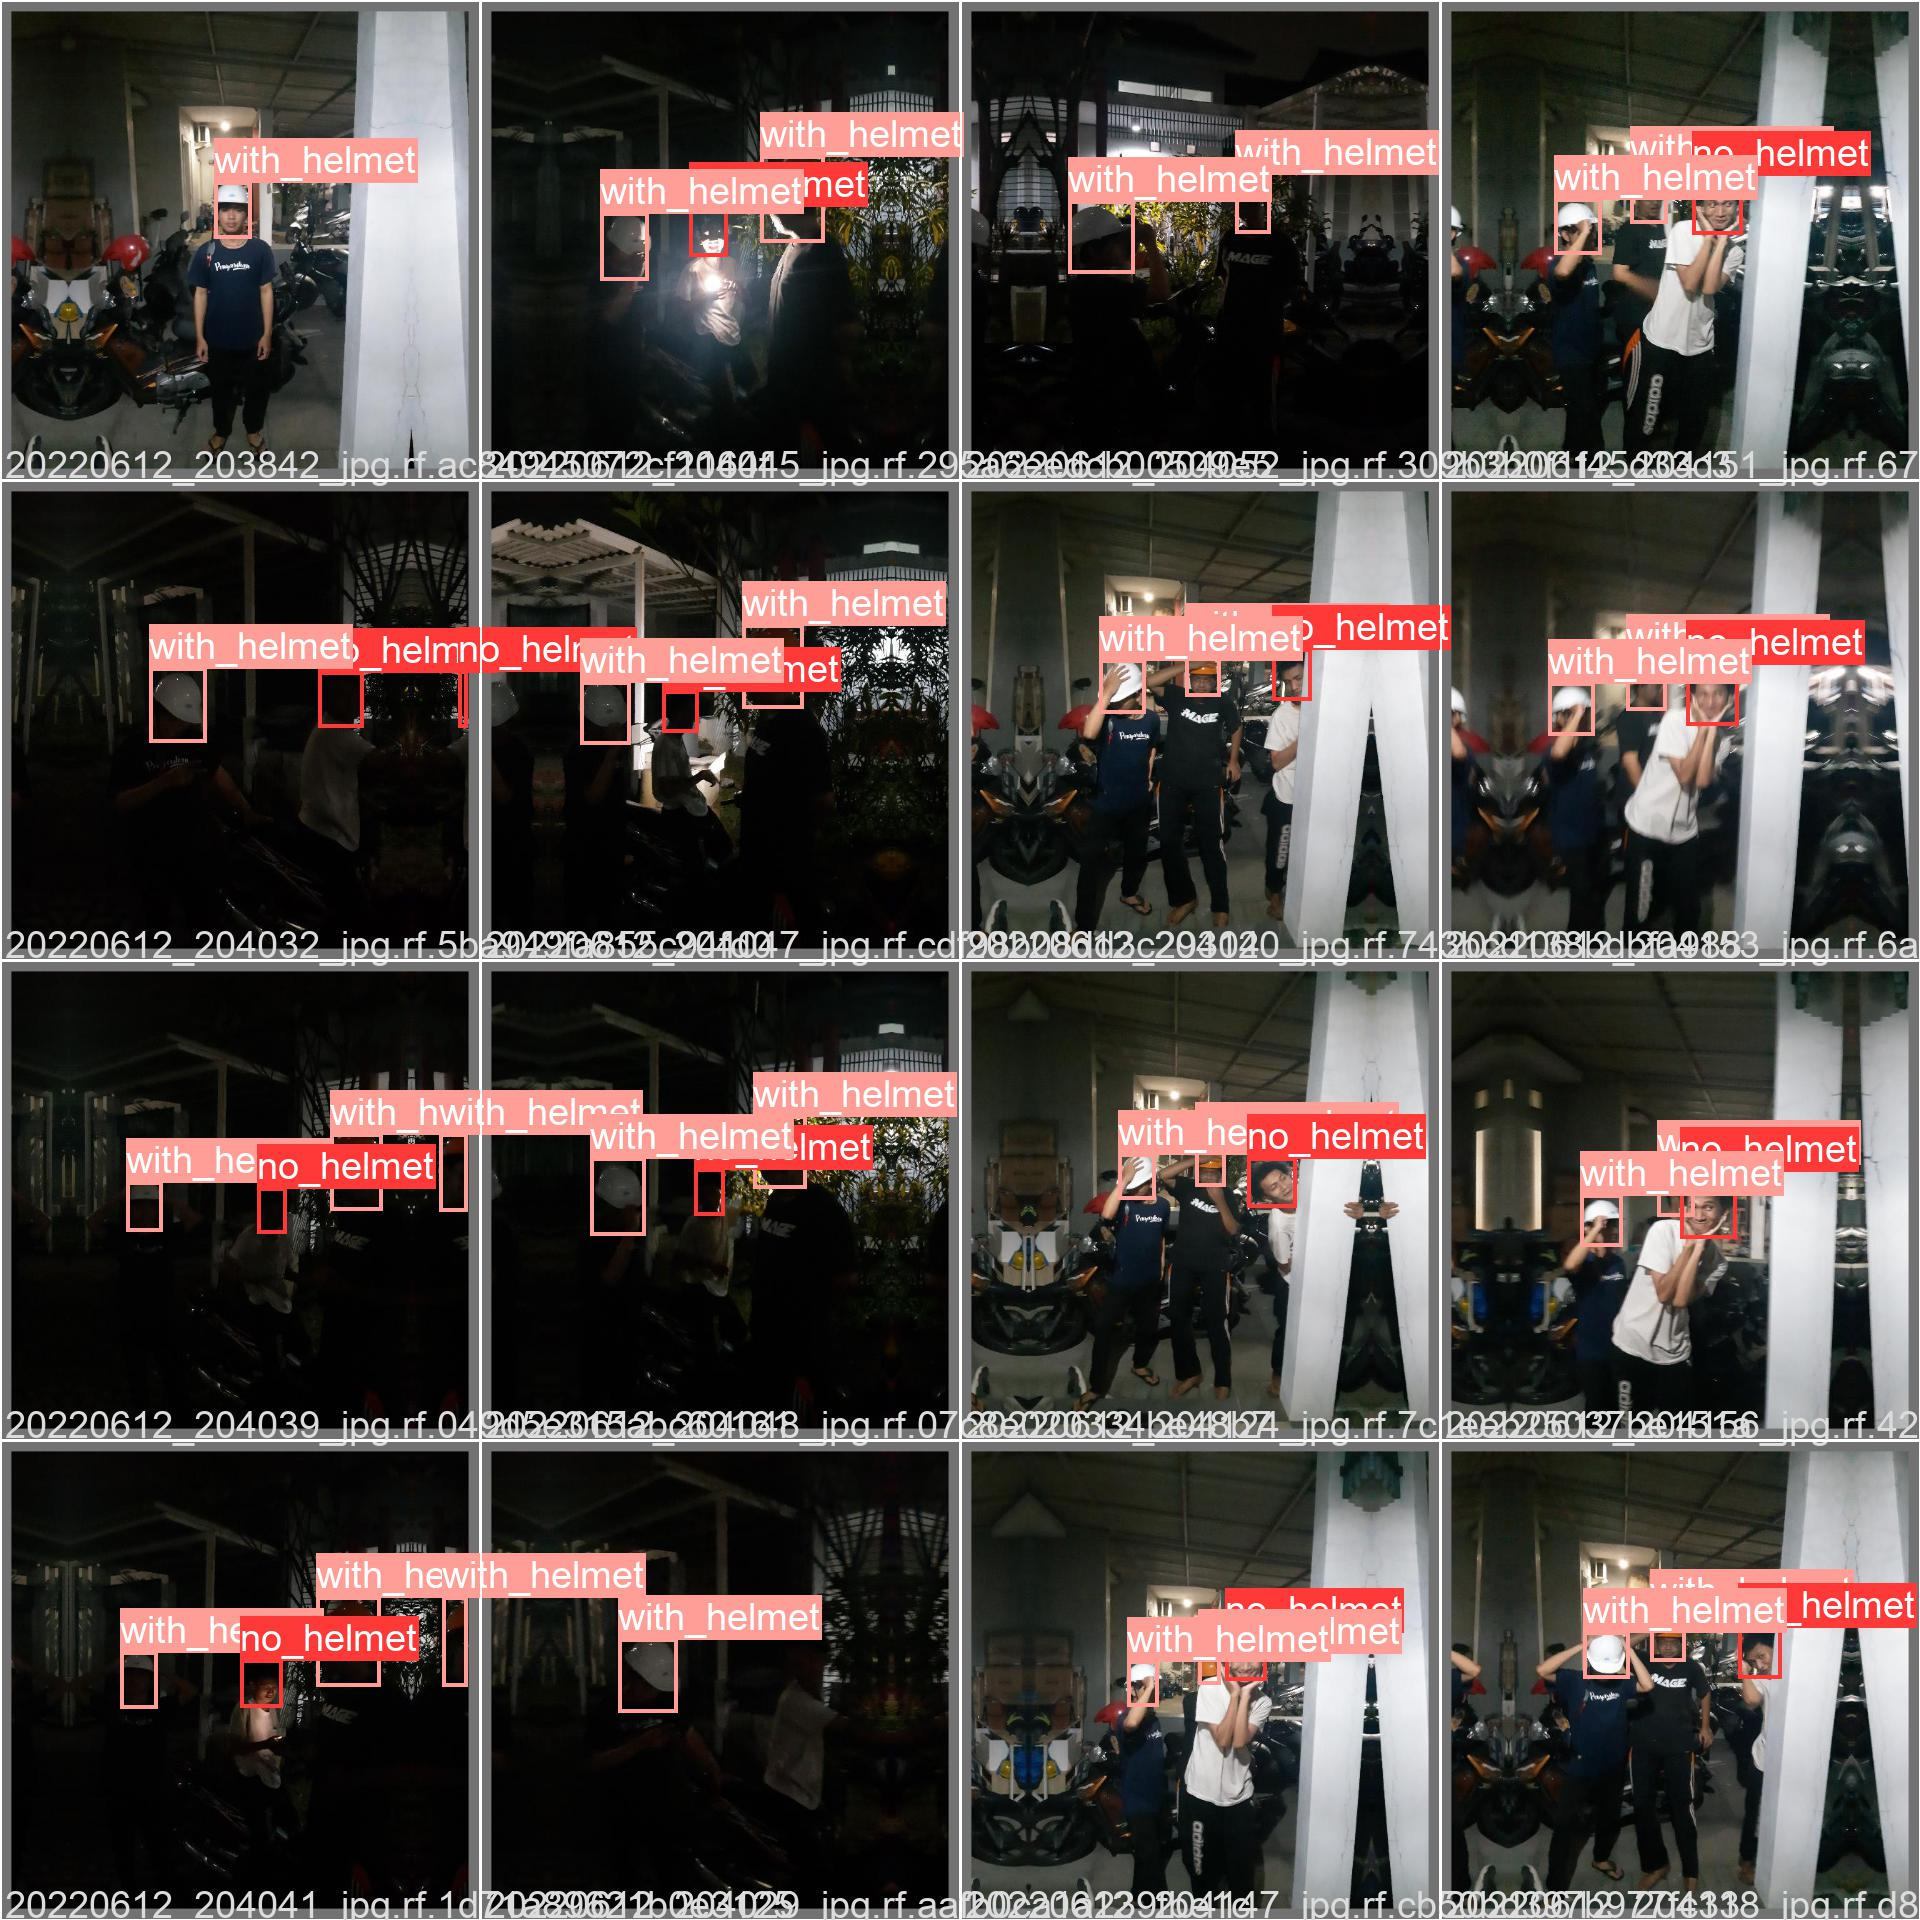
\includegraphics[scale=0.1]{gambar/train_v2_val/low_ligjt/yolosmall/lowlight_val_batch0_labels.jpg}
    \caption{Hasil Prediksi Pada Keadaan dengan hedec\textunderscore pretrain\textunderscore S}
    % \label{fig:labelbaru}  
  \end{figure}


  
  \item \textbf{hedec\textunderscore pretrain\textunderscore M} 
  
  \par Dilakukan pengujian kecerahan rendah dengan menggunakan bobot yang di-\emph{train} menggunakan bobot
  pretrain COCO untuk varian \emph{medium}. Didapatkan rata - rata presisi untuk semua kelas 0.833 dan \emph{recall} untuk semua
  kelas 0.831. Didapati hasil \emph{precision} dan \emph{recall} untuk kelas \emph{no\textunderscore helm} ,yang biasanya
  memiliki nilai yang kurang bagus pada varian bobot nano , mendapatkan nilai 1 dan 0.68 yang dimana lebih bagus. 
  Varian Medium ini merupakan varian yang memiliki hasil validasi paling tinggi untuk \emph{precision} dan \emph{recall} nya diantara semua \emph{weight}
  yang di \emph{train} menggunakan \emph{pretrained weights} dari YOLOv5 bahkan melebihi varian YOLOv5l yang akan dipaparkan di bagian selanjutnya.
  \newpage
  \begin{longtable}{|c|c|c|c|}
    \caption{Hasil Validasi Pada Tingkat Kecerahan Rendah dengan hedec\textunderscore pretrain\textunderscore M}
    \label{tb:validasitingkatacerahrendah_yolov5m}\\
    \hline
    % \rowcolor[HTML]{C0C0C0}
    \textbf{\emph{Class} }                     & \textbf{\emph{Precision}}  & \textbf{\emph{Recall}} & \textbf{\emph{mAP@.5}}\\
    \hline
    all                                                 & 0.833          & 0.831       & 0.893         \\
    no\textunderscore helmet                            & 1              & 0.68        & 0.814         \\
    with\textunderscore helmet                          & 0.666          & 0.982       & 0.973         \\
    \hline
  \end{longtable}

  
  \begin{figure} [h!]
    \centering
    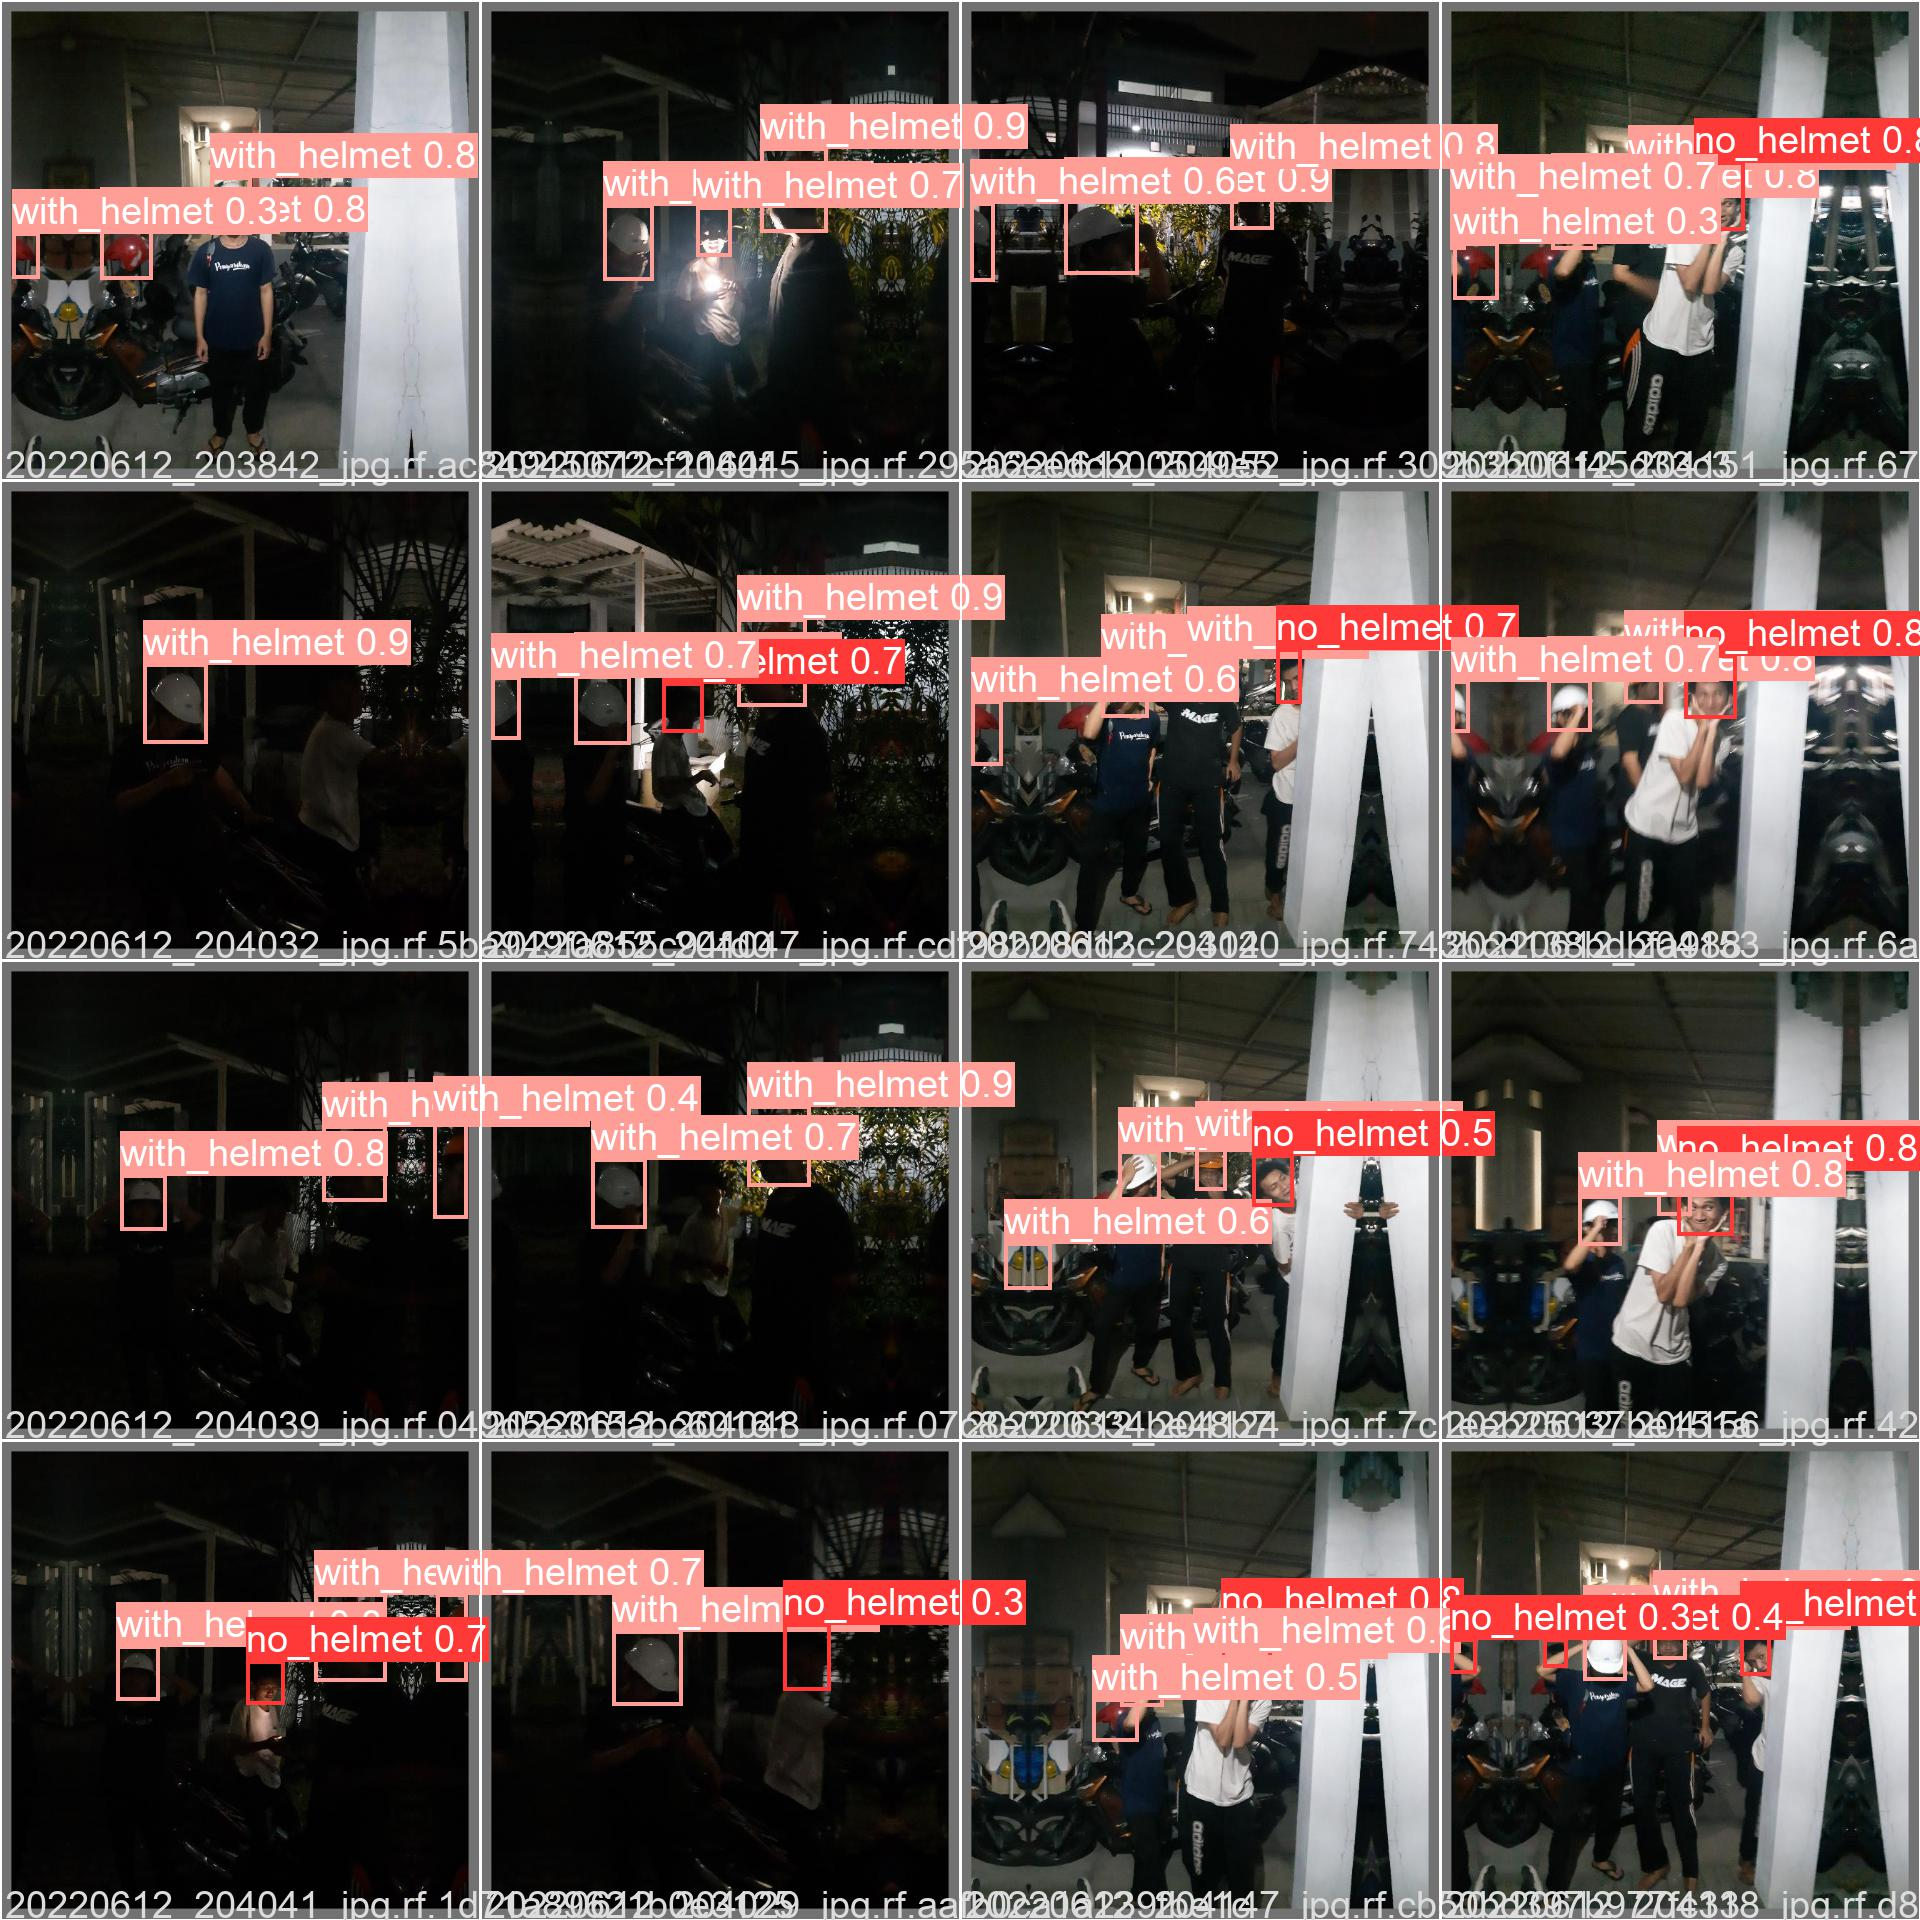
\includegraphics[scale=0.2]{gambar/train_v2_val/low_ligjt/yolomedium/val_batch0_pred.jpg}
    % \includegraphics[scale=0.1]{gambar/train_v2_val/low_ligjt/yolomedium/val_batch0_labels.jpg}
    \caption{Hasil Prediksi Pada Keadaan dengan hedec\textunderscore pretrain\textunderscore M}
    % \label{fig:labelbaru}  
  \end{figure}


  \item \textbf{hedec\textunderscore pretrain\textunderscore L}
  
  \par Dilakukan pengujian kecerahan rendah dengan menggunakan bobot yang di-\emph{train} menggunakan bobot
  pretrain COCO untuk varian \emph{large}. Didapatkan rata - rata presisi untuk semua kelas 0.811 dan \emph{recall} untuk semua
  kelas 0.765 dimana lebih kecil dibandingkan varian \emph{medium}. Didapati juga hasil \emph{precision} dan \emph{recall} untuk kelas \emph{no\textunderscore helm} yang mengalami penurunan dibanding
  menggunakan variant \emph{medium} yaitu 0.914 untuk \emph{precision} dan 0.6 untuk \emph{recall}. Selain itu untuk
  \emph{inference time} nya tentu saja mengalami kenaikan dibandingan dengan varian - varian sebelumnya yang lebih kecil.
  
  \begin{longtable}{|c|c|c|c|}
    \caption{Hasil Validasi Pada Tingkat Kecerahan Rendah dengan hedec\textunderscore pretrain\textunderscore L}
    \label{tb:validasitingkatacerahrendah_yolov5l}\\
    \hline
    % \rowcolor[HTML]{C0C0C0}
    \textbf{\emph{Class} }                     & \textbf{\emph{Precision}}  & \textbf{\emph{Recall}} & \textbf{\emph{mAP@.5}}\\
    \hline
    all                                                 & 0.811          & 0.765       & 0.893         \\
    no\textunderscore helmet                            & 0.914          & 0.6         & 0.724         \\
    with\textunderscore helmet                          & 0.708          & 0.93        & 0.931         \\
    \hline
  \end{longtable}
  
  \begin{figure} [h!]
    \centering
    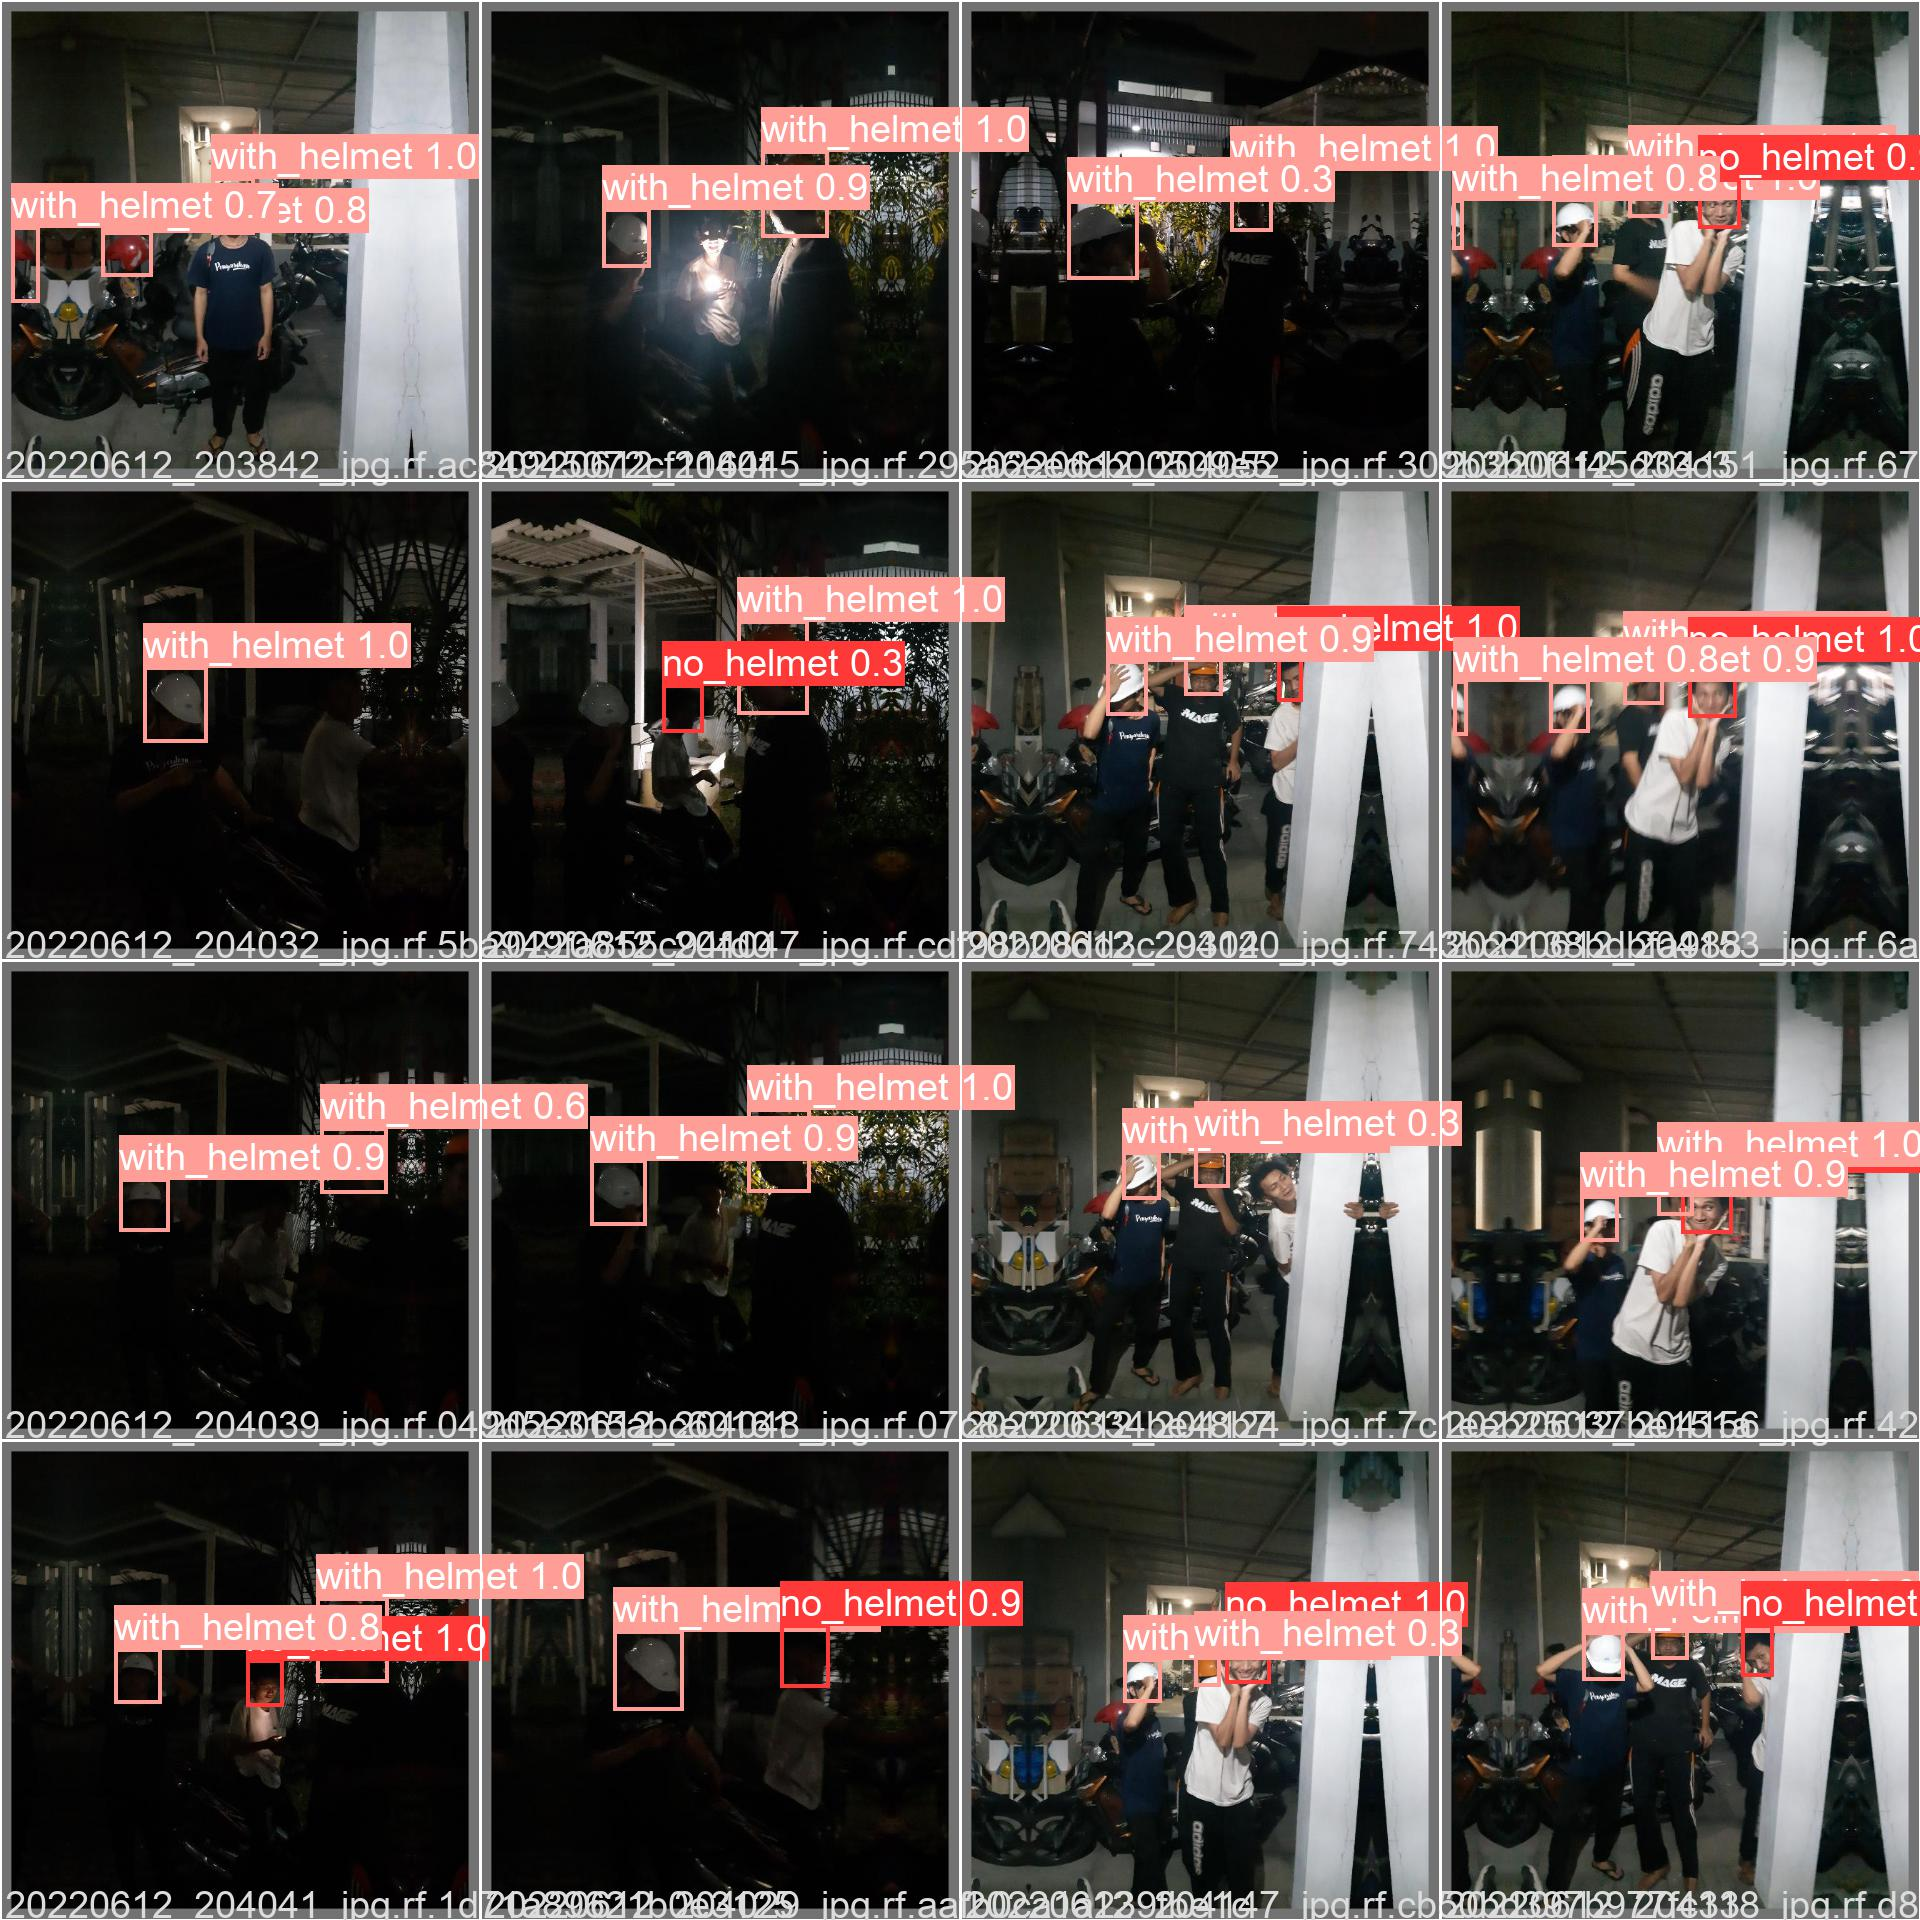
\includegraphics[scale=0.2]{gambar/train_v2_val/low_ligjt/yololarge/val_batch0_pred.jpg}
    % \includegraphics[scale=0.1]{gambar/train_v2_val/low_ligjt/yololarge/val_batch0_labels.jpg}
    \caption{Hasil Prediksi Pada Keadaan dengan hedec\textunderscore pretrain\textunderscore Ll}
    % \label{fig:labelbaru}  
  \end{figure}

\end{enumerate}


\subsection{Pengujian Pada Tingkat Kecerahan Rendah dengan \emph{Weight} Murni Deteksi Helm Keselamatan Kerja}
\label{subsec:lowlight_pure}

\par Berikut merupakan pemaparan hasil validasi menggunakan data validasi pada keadaan minim pencahayaan menggunakan
\emph{weight} yang merupakan hasil \emph{train} dari dataset Deteksi Helm Keselamatan Kerja tanpa menggunakan \emph{pretrained weight}.
Hasil \emph{train} tanpa menggunakan \emph{pretrain weight} ini selanjutkan akan disebut sebagai "hedec\textunderscore pure".

 

\begin{enumerate}
  \newpage
  \item \textbf{hedec\textunderscore pure\textunderscore N } 
  
  \par Dilakukan pengujian kecerahan rendah dengan menggunakan bobot yang di-\emph{train} tanpa menggunakan bobot
  pretrain COCO tetapi konfigurasi modelnya dibuat serupa dengan konfigurasi YOLOv5n. 
  Didapatkan rata - rata presisi untuk semua kelas 0.659   dan \emph{recall} untuk semuakelas 0.696.
  \par  Sewajarnya varian ini mendapatkan nilai \emph{precision} dan \emph{recall} paling kecl diantara varian lainnya dan juga \emph{inference speed}
  yang paling cepat dibanding varian lainnya pada \emph{weight} murni \emph{tanpa pretrained weight}.
  
  \begin{longtable}{|c|c|c|c|}
    \caption{Hasil Validasi Pada Tingkat Kecerahan Rendah dengan \emph{Hedec Nano}}
    \label{tb:validasitingkatacerahrendah_hedecN}\\
    \hline
    % \rowcolor[HTML]{C0C0C0}
    \textbf{\emph{Class} }                     & \textbf{\emph{Precision}}  & \textbf{\emph{Recall}} & \textbf{\emph{mAP@.5}}\\
    \hline
    all                                                 & 0.659          & 0.696        & 0.731         \\
    no\textunderscore helmet                            & 0.76           & 0.55         & 0.621         \\
    with\textunderscore helmet                          & 0.558          & 0.842        & 0.842         \\
    \hline
  \end{longtable}
  
  \begin{figure}[h]
    \centering
    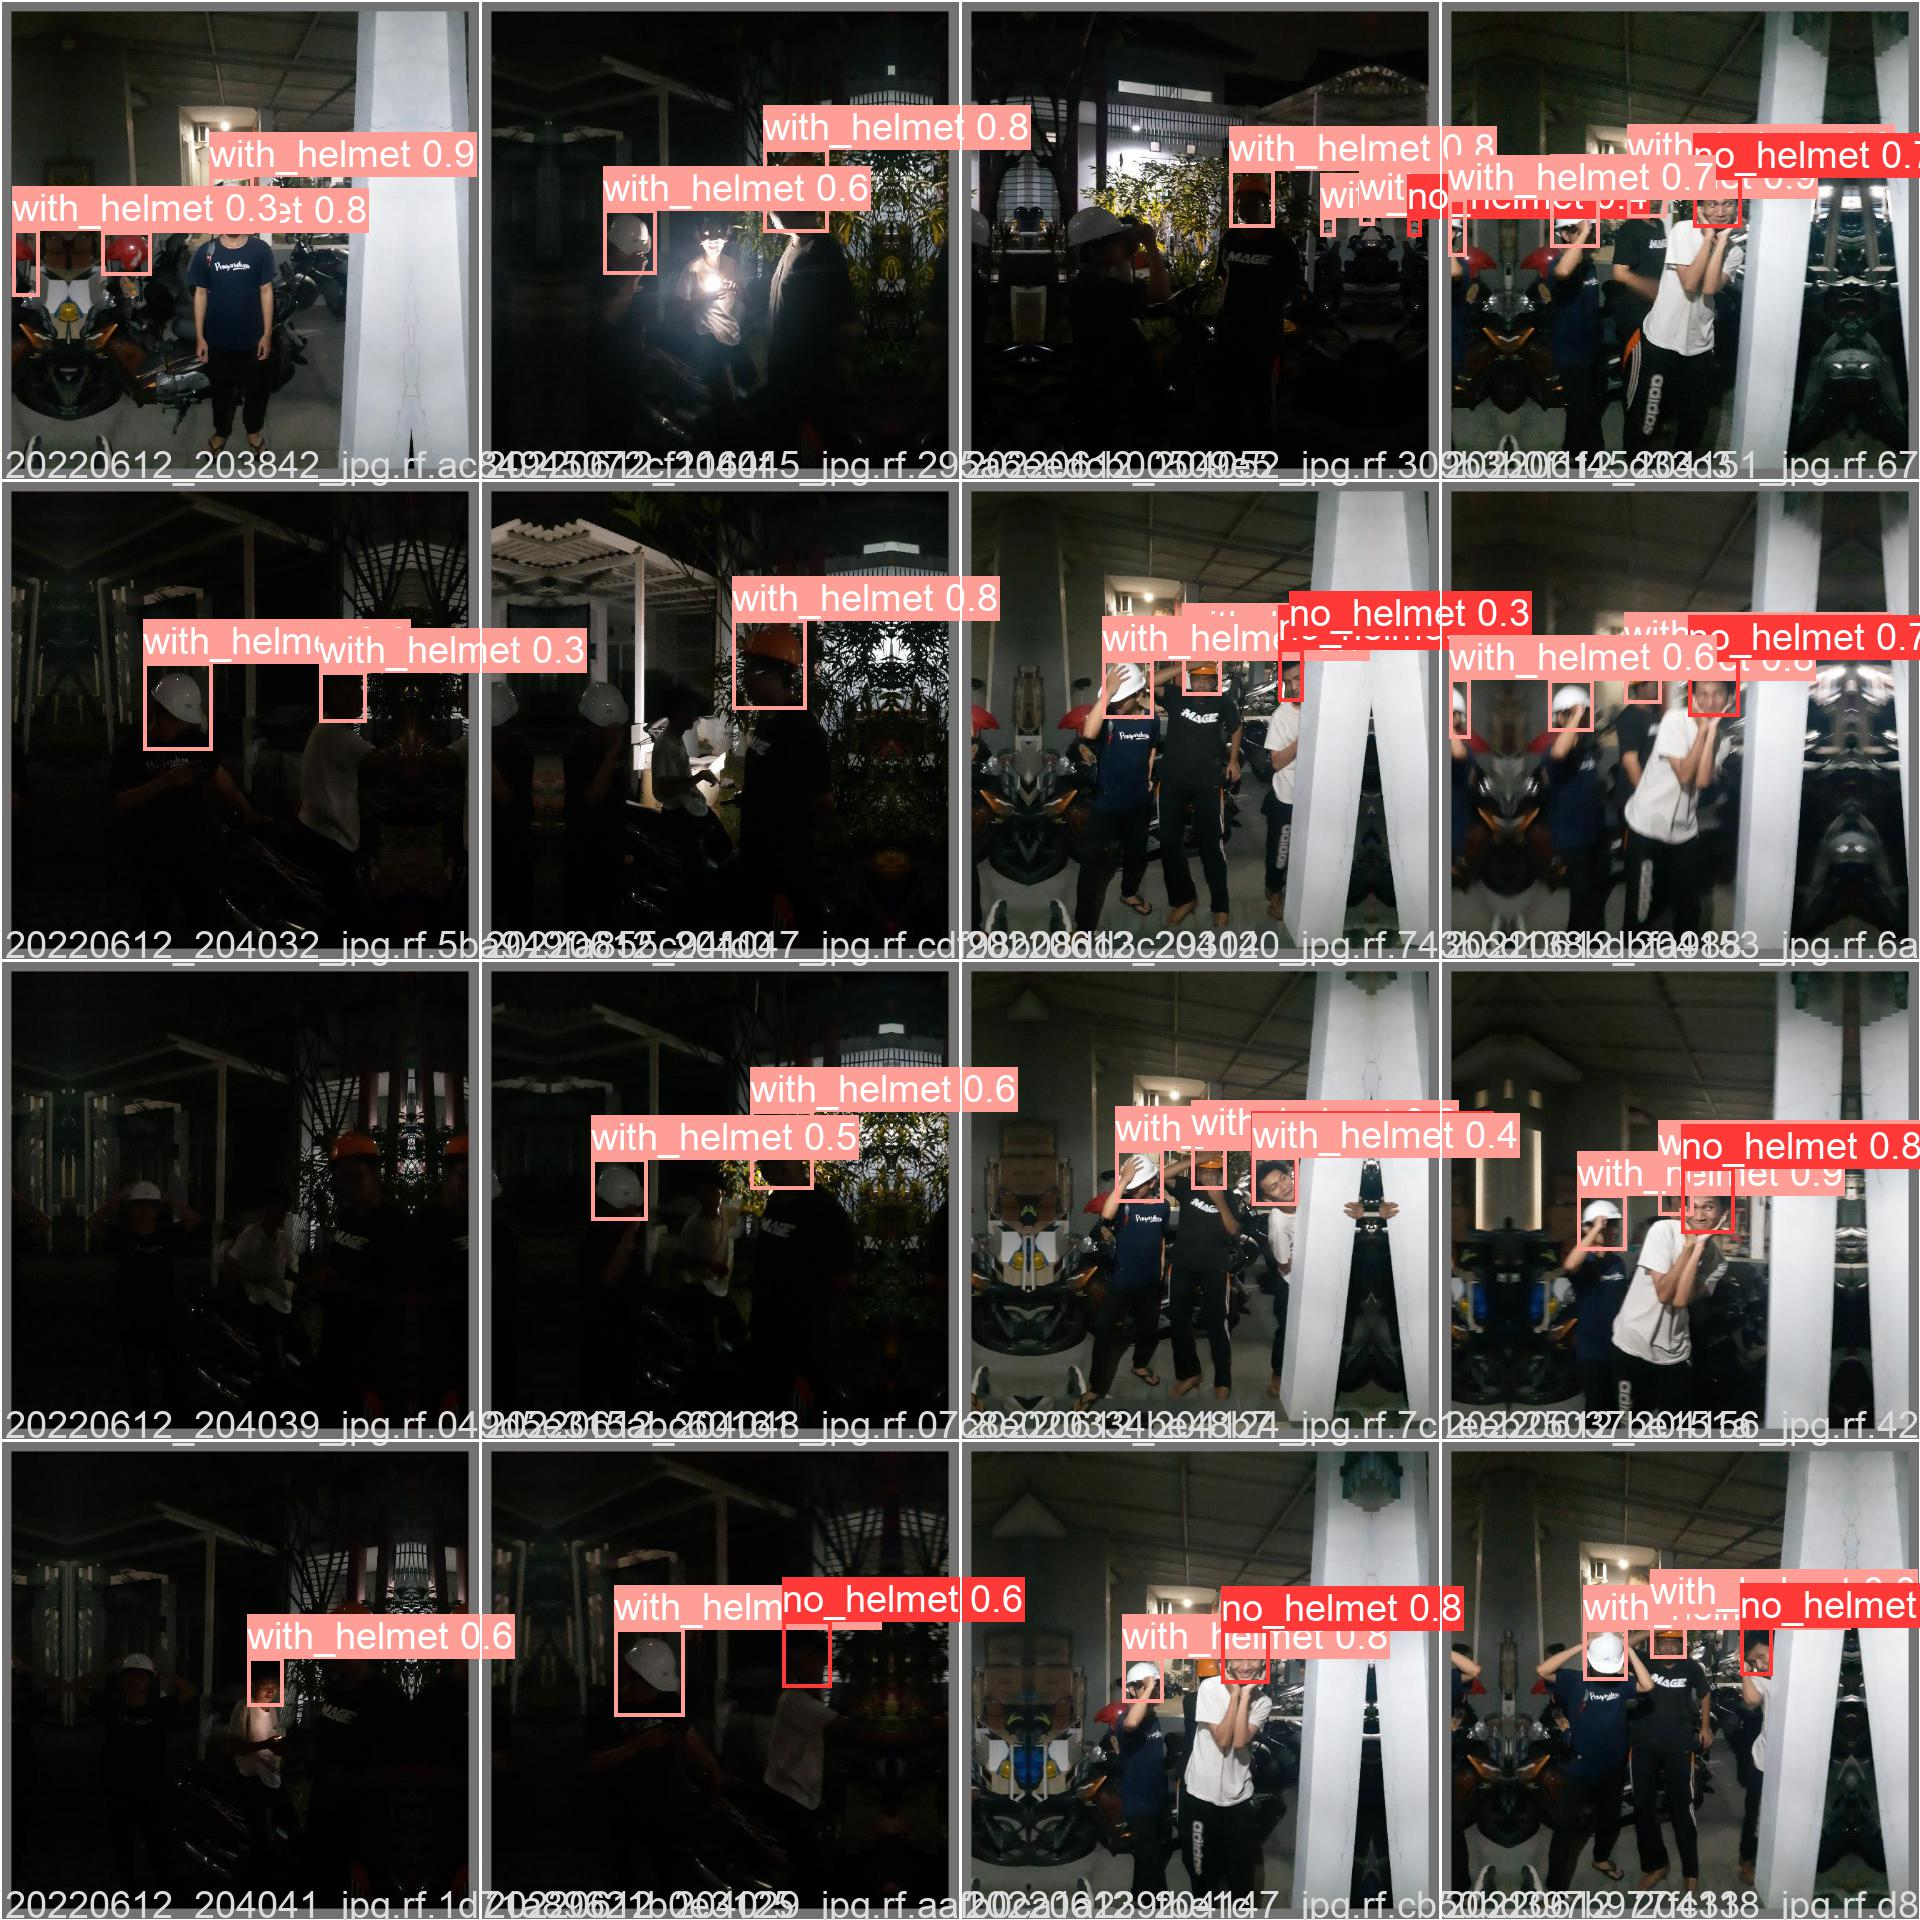
\includegraphics[scale=0.2]{gambar/train_v2_val/low_ligjt/customNano/val_batch0_pred.jpg}
    % \includegraphics[scale=0.1]{gambar/train_v2_val/low_ligjt/customNano/val_batch0_labels.jpg}
    \caption{Hasil Prediksi Pada Keadaan dengan \emph{Weight Hedec Nano}}
    % \label{fig:labelbaru}  
  \end{figure}
  
  
  \item \textbf{hedec\textunderscore pure\textunderscore S }
  
  \par Dilakukan pengujian kecerahan rendah dengan menggunakan bobot yang di-\emph{train} tanpa menggunakan bobot
  pretrain COCO tetapi konfigurasi modelnya dibuat serupa dengan konfigurasi YOLOv5s. 
  Didapatkan rata - rata presisi untuk semua kelas 0.706   dan \emph{recall} untuk semuakelas 0.696 dimana sedikit lebih baik
  dibandingkan varian \emph{Nano} sebelumnya.
  
  \begin{longtable}{|c|c|c|c|}
    \caption{Hasil Validasi Pada Tingkat Kecerahan Rendah dengan \emph{Hedec Small}}
    \label{tb:validasitingkatacerahrendah_hedecS}\\
    \hline
    % \rowcolor[HTML]{C0C0C0}
    \textbf{\emph{Class} }                     & \textbf{\emph{Precision}}  & \textbf{\emph{Recall}} & \textbf{\emph{mAP@.5}}\\
    \hline
    all                                                 & 0.706          & 0.696        & 0.847         \\
    no\textunderscore helmet                            & 0.885          & 0.771        & 0.789         \\
    with\textunderscore helmet                          & 0.623          & 0.947        & 0.905         \\
    \hline
  \end{longtable}
  
  \begin{figure} [h!]
    \centering
    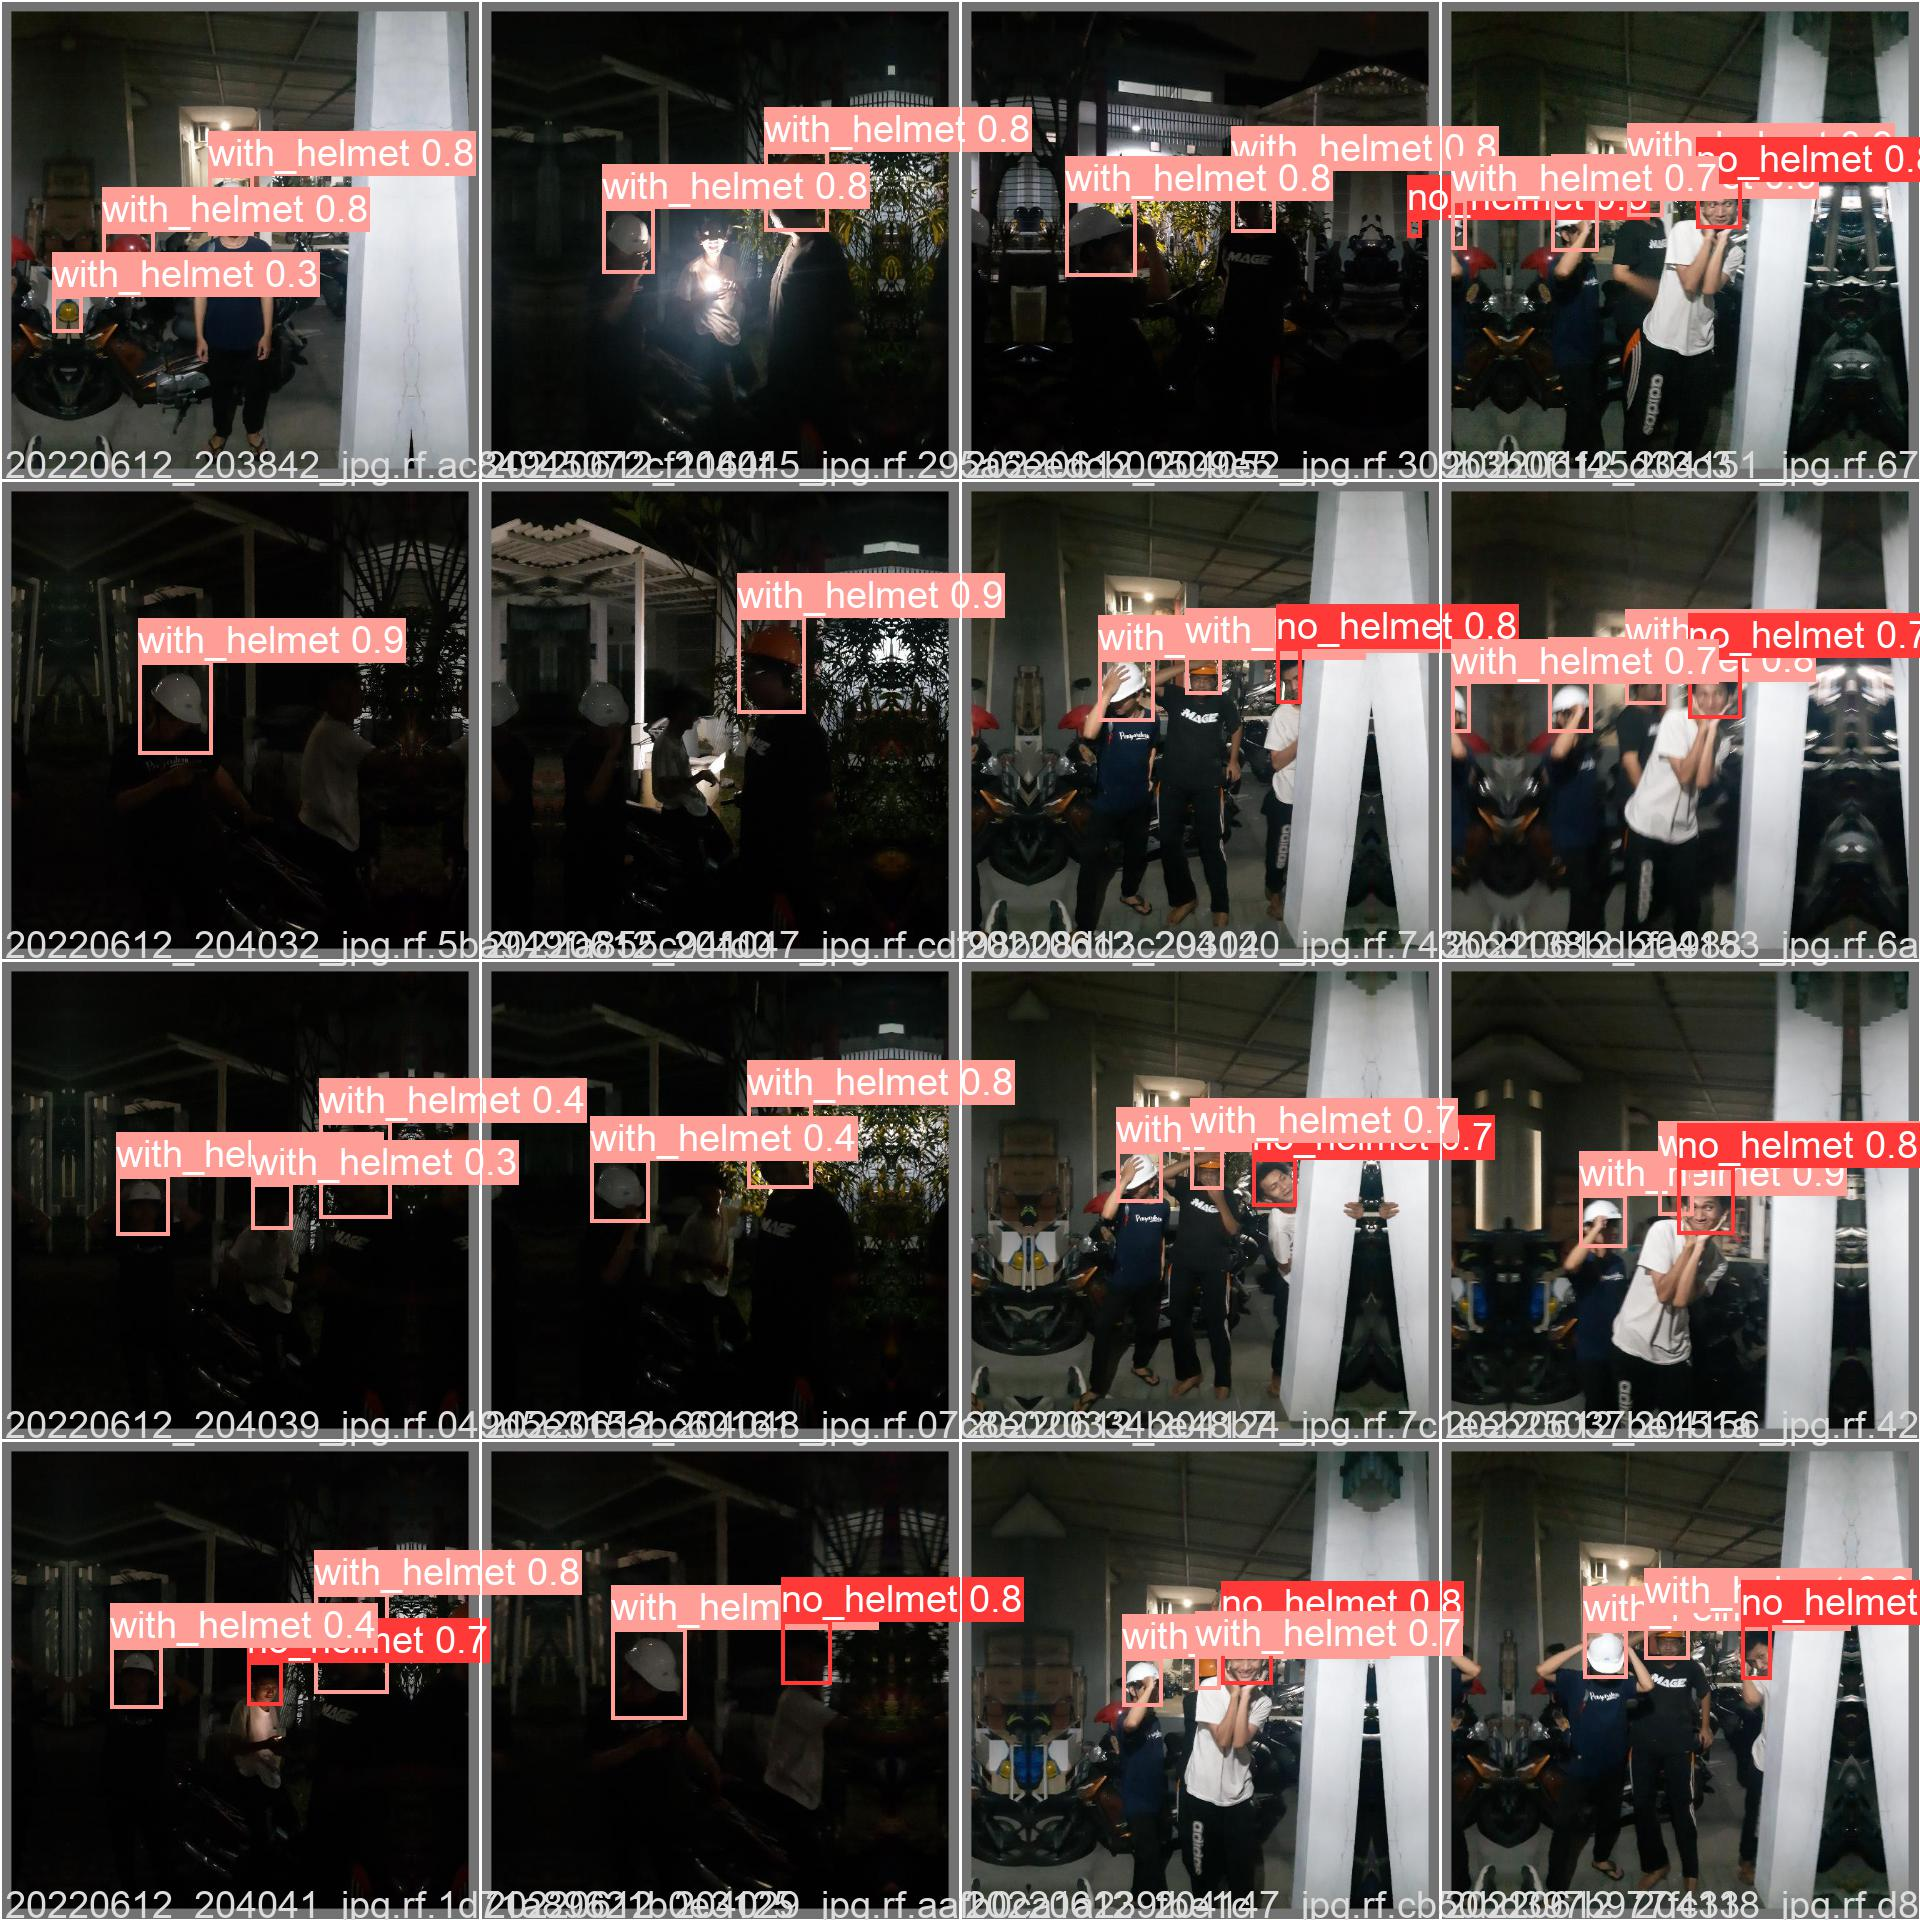
\includegraphics[scale=0.2]{gambar/train_v2_val/low_ligjt/customSmall/val_batch0_pred.jpg}
    % \includegraphics[scale=0.1]{gambar/train_v2_val/low_ligjt/customSmall/val_batch0_labels.jpg}
    \caption{Hasil Prediksi Pada Keadaan dengan \emph{Weight Hedec Small}}
    % \label{fig:labelbaru}  
  \end{figure}

   \newpage
  \item \textbf{hedec\textunderscore pure\textunderscore M }
  
  \par Dilakukan pengujian kecerahan rendah dengan menggunakan bobot yang di-\emph{train} tanpa menggunakan bobot
  pretrain COCO tetapi konfigurasi modelnya dibuat serupa dengan konfigurasi YOLOv5m. 
  Didapatkan rata - rata presisi untuk semua kelas 0.731   dan \emph{recall} untuk semuakelas 0.862 dimana lebih baik dibandingkan
  varian \emph{Small}.
  
  \begin{longtable}{|c|c|c|c|}
    \caption{Hasil Validasi Pada Tingkat Kecerahan Rendah dengan \emph{Hedec Medium}}
    \label{tb:validasitingkatacerahrendah_hedecM}\\
    \hline
    % \rowcolor[HTML]{C0C0C0}
    \textbf{\emph{Class} }                     & \textbf{\emph{Precision}}  & \textbf{\emph{Recall}} & \textbf{\emph{mAP@.5}}\\
    \hline
    all                                                 & 0.731          & 0.862       & 0.827         \\
    no\textunderscore helmet                            & 0.799          & 0.793       & 0.757         \\
    with\textunderscore helmet                          & 0.663          & 0.93        & 0.897         \\
    \hline
  \end{longtable}
  
  \begin{figure} [h!]
    \centering
    \includegraphics[scale=0.2]{gambar/train_v2_val/low_ligjt/customMedium/val_batch0_pred.jpg}
    % \includegraphics[scale=0.1]{gambar/train_v2_val/low_ligjt/customMedium/val_batch0_labels.jpg}
    \caption{Hasil Prediksi Pada Keadaan dengan \emph{Weight Hedec Medium}}
    % \label{fig:labelbaru}  
  \end{figure}
  
  \newpage
  \item \textbf{hedec\textunderscore pure\textunderscore L }
  \par Dilakukan pengujian kecerahan rendah dengan menggunakan bobot yang di-\emph{train} tanpa menggunakan bobot
  pretrain COCO tetapi konfigurasi modelnya dibuat serupa dengan konfigurasi YOLOv5l. 
  Didapatkan rata - rata presisi untuk semua kelas 0.743   dan \emph{recall} untuk semuakelas 0.755.
  \par Berbeda dengan bobot imbangan variasi \emph{Large} yang dilatih menggunakan Pretrained COCO, \emph{overall precision} pada varian ini
  sedikit lebih baik daripada varian \emph{Medium} nya, tetapi untuk \emph{Recall} sama - sama lebih kecil.
  
   
  \begin{longtable}{|c|c|c|c|}
    \caption{Hasil Validasi Pada Tingkat Kecerahan Rendah dengan \emph{Hedec Large}}
    \label{tb:validasitingkatacerahrendah_hedecL}\\
    \hline
    % \rowcolor[HTML]{C0C0C0}
    \textbf{\emph{Class} }                     & \textbf{\emph{Precision}}  & \textbf{\emph{Recall}} & \textbf{\emph{mAP@.5}}\\
    \hline
    all                                                 & 0.743          & 0.755       & 0.789         \\
    no\textunderscore helmet                            & 0.85           & 0.65        & 0.733         \\
    with\textunderscore helmet                          & 0.663          & 0.86        & 0.845         \\
    \hline
  \end{longtable}
  
  \begin{figure} [h!]
    \centering
    \includegraphics[scale=0.2]{gambar/train_v2_val/low_ligjt/customLarge/val_batch0_pred.jpg}
    % \includegraphics[scale=0.1]{gambar/train_v2_val/low_ligjt/customLarge/val_batch0_labels.jpg}
    \caption{Hasil Prediksi Pada Keadaan dengan \emph{Weight Hedec Large}}
    % \label{fig:labelbaru}  
  \end{figure}
  
\end{enumerate}

\subsection{Analisis Pengujian Pada Pencahayaan Rendah}
  \label{subsec:analisis_lowlight}

  \begin{figure} [h!]
    \centering
    \includegraphics[width=1.0\textwidth]{gambar/lowlight_grafic/Low Light - all.png}
    \caption{Grafik Hasil Testing Pada Pencahayaan Rendah untuk Semua Kelas}
    \label{fig:graf_lowlight_all}  
  \end{figure}

  \begin{figure} [h!]
    \centering
    \includegraphics[width=.45\textwidth]{gambar/lowlight_grafic/Low Light - no_helmet.png}
    \includegraphics[width=.45\textwidth]{gambar/lowlight_grafic/Low Light - with_helmet.png}
    \caption{Grafik Hasil Testing Pada Pencahayaan Rendah untuk Masing - Masing Kelas}
    \label{fig:graf_lowlight_eachclass}  
  \end{figure}

  \par Berdasarkan hasil yang sudah diaparkan untuk bobot varian hasil 
  pretrain dan murni tanpa pretrain yang diapaprkan pada Subbab~\ref{subsec:lowlight_pretrained} 
  dan Subbab~\ref{subsec:lowlight_pure}, dapat ditarik beberapa point. Varian bobot "hedec\_pretrain\_N"
  memiliki nilai \emph{recall} paling rendah dari semua bobot dikarenakan kegagalan dalam mendeteksi
  kelas "no\_helmet" pada dataset testing yang disediakan. Secara umum, bobot yang paling bagus digunakan
  pada kasus pencahayaan rendah terdapat pada bobot "hedec\_pretrain\_L" yang merupakan
  bobot yang dilatih menggunakan\emph{pretrained weights}" untuk varian yolov5l yang memiliki
  \emph{"depth\_multiplier"} dan "\emph{width\_multiplier}" paling besar. Selain itu, seperti yang
  ditunjukkan pada Gambar~\ref{fig:graf_lowlight_all} untuk varian yang menggunakan
  \emph{pretrained weights} jika diurutkan dari varian \emph{Nano} hingga \emph{Large} selalu mengalami
  kenaikan nilai mAP.5 nya. Tetapi untuk varian yang dilatih murni hanya menggunakan Dataset Helm Keselamatan Kerja
  mengalami kenaikan nilai mAP.5 hanya sampai pada varian \emph{Small (S)} dan setelah itu mengalami penurunan hingga varian \emph{Large (L)}.



\section{Pengujian Model YOLOv5 dengan \emph{Helmet Detection Weights} Pada Jetson Nano}
\label{sec:jetsonnano_hedectest}

\par Bagian ini merupakan pemaparan hasil pengujian performa Model YOLOv5 dengan bobot - bobot yang sudah di\emph{train}
sebelumnya pada Jetson Nano. Tujuan dari pengujian ini yaitu membandingkan effektifitas dari masing - masing
bobot yang sudah dibuat pada aspek performa \emph{inference} mengingat Jetson Nano merupakan \emph{mini-computer} yang memiliki
\emph{Graphic Processing Unit}(GPU)nya sendiri dan memang didesain untuk aplikasi AI IoT. Pengujuran yang diambil pada pengujian ini
yaitu nilai \emph{Frame Per Second}(FPS).

 
\par Pengujian dilakukan menggunakan Webcam Nemesis NYK A-90 Everest yang dipasang dengan Jetson Nano melalui kabel USB. 
Pengujian dilakukan pada resolusi 256, 480, dan 640. Hasil pengukuran FPS pada pengujian YOLOv5 Helmet Detection dipaparkan pada Tabel~\ref{tb:jetsonanoperformancetest}.



\begin{longtable}{|l|l|l|l|} 
  \caption{Hasil Test Peforma Pad Jetson Nano}
  \label{tb:jetsonanoperformancetest}\\
  \hline
  \multirow{2}{*}{\textbf{Nama Bobot}} & \multicolumn{3}{l|}{\textbf{Resolusi}}      \\ 
  \cline{2-4}
                                       & \textbf{256} & \textbf{480} & \textbf{640}  \\ 
  \hline
  hedec\_pretrain\_N                   & 24.4         & 22           & 18.5          \\
  hedec\_pretrain\_S                   & 22.2         & 13           & 7.8           \\
  hedec\_pretrain\_M                   & 15.2         & 5.7          & 3.4           \\
  hedec\_pretrain\_L                   & 8            & 3.2          & 1.8           \\
  hedec\_pure\_N                       & 24.9         & 21.5         & 18.4          \\
  hedec\_pure\_S                       & 23           & 12.3         & 7.8           \\
  hedec\_pure\_M                       & 15           & 5.4          & 3.3           \\
  hedec\_pure\_L                       & 8.3          & 3            & 1.8           \\
  \hline
\end{longtable}

\begin{figure} [h!]
  \centering
  \includegraphics[width=.45\textwidth]{gambar/performance_jetson/Frame Rate Hedec_Pretrain di Jetson Nano.png}
  \includegraphics[width=.45\textwidth]{gambar/performance_jetson/Frame Rate Hedec_Puredi Jetson Nano.png}
  \caption{Grafik Performa berdasarkan Frame Rate Pada Jetson Nano Untuk "Hedec\_pretrain" dan "Hedec\_pure"}
  \label{fig:graf_jetsonano}  
\end{figure}

\FloatBarrier

\par Berdasarkan hasil pengujian pada ~\ref{tb:jetsonanoperformancetest}, terdapat beberapa poin analisis yang bisa diambil.
Performa dari nilai \emph{Frame Rate} dari \emph{weight} yang menggunakan \emph{Pretrained Weights} dengan pasangan bandingnya di \emph{weight}
yang tidak menggunakan \emph{Pretrained Weights} memiliki performa yang tidak berbeda jauh. Sewajarnya, varian \emph{Nano (N)} dari
\emph{Pretrained Weight} atau \emph{Pure Weight} memiliki FPS paling tinggi dibandingkan varian diatasnya yaitu S,M,dan L.